\documentclass[
    a4paper,
    fontsize=12pt,
    footinclude=true,
    headinclude=true
	]{scrbook}

	\usepackage{scrhack}
	\usepackage{silence}
	\WarningFilter{latex}{You have requested package}
	\usepackage{template/preamble}
	\setlength{\parskip}{0.3em}

\bibliography{biblio.bib}


\usepackage{ifthen}
\usepackage{adjustbox}
\usepackage{graphicx}
\usepackage{comment}
\usepackage{svg}
\usepackage{amsmath,amssymb} % define this before the line numbering.
\usepackage{color, colortbl}
\usepackage[dvipsnames]{xcolor}
\usepackage{nicefrac}
\usepackage{booktabs}
\usepackage{placeins}
\usepackage{pifont}
\usepackage{subcaption}
\usepackage{xspace}
\usepackage{gensymb}
\usepackage{arydshln}
\usepackage{nicefrac}
\usepackage{algorithm}
\usepackage{algpseudocode}
\algrenewcommand\algorithmicindent{1.0em}%
\usepackage{epigraph}
\usepackage{listings}
\usepackage{bibentry}
\usepackage{makecell}
\usepackage{float}
\usepackage{lineno}
\linenumbers

% for an adaptable epigraph
\renewcommand{\epigraphsize}{\small}
\setlength{\epigraphwidth}{0.6\textwidth}
\renewcommand{\textflush}{flushright}
\renewcommand{\sourceflush}{flushright}
% A useful addition
\newcommand{\epitextfont}{\itshape}
\newcommand{\episourcefont}{\scshape}

\makeatletter
\newsavebox{\epi@textbox}
\newsavebox{\epi@sourcebox}
\newlength\epi@finalwidth
\renewcommand{\epigraph}[2]{%
  \vspace{\beforeepigraphskip}
  {\epigraphsize\begin{\epigraphflush}
   \epi@finalwidth=\z@
   \sbox\epi@textbox{%
     \varwidth{\epigraphwidth}
     \begin{\textflush}\epitextfont#1\end{\textflush}
     \endvarwidth
   }%
   \epi@finalwidth=\wd\epi@textbox
   \sbox\epi@sourcebox{%
     \varwidth{\epigraphwidth}
     \begin{\sourceflush}\episourcefont#2\end{\sourceflush}%
     \endvarwidth
   }%
   \ifdim\wd\epi@sourcebox>\epi@finalwidth 
     \epi@finalwidth=\wd\epi@sourcebox
   \fi
   \leavevmode\vbox{
     \hb@xt@\epi@finalwidth{\hfil\box\epi@textbox}
     \vskip1.75ex
     \hrule height \epigraphrule
     \vskip.75ex
     \hb@xt@\epi@finalwidth{\hfil\box\epi@sourcebox}
   }%
   \end{\epigraphflush}
   \vspace{\afterepigraphskip}}}
\makeatother


\newcommand{\titlecaption}[3][]{\caption[#2]{\textbf{#2}\ifthenelse{\equal{#1}{}}{. }{ }#3}}

\newcommand{\todo}[1]{\textcolor{BrickRed}{[TODO #1]}}
\newcommand{\note}[1]{\textcolor{PineGreen}{(#1)}}
\newcommand{\review}[1]{\textcolor{RoyalBlue}{#1}}
\newcommand{\startreview}{\color{RoyalBlue}}
\newcommand{\stopreview}{\color{black}}
\newcommand\Tstrut{\rule{0pt}{2.6ex}}         % = `top' strut
\newcommand\Bstrut{\rule[-0.9ex]{0pt}{0pt}}   % = `bottom' stru
\newcommand{\mypm}{\,$\pm$\,}
\newcommand{\mysmpm}[1]{\scriptsize{\mypm#1}}
\newcommand{\minipar}[1]{\noindent \textbf{#1}}
\def\mypar#1{\vspace{1mm}{\noindent\textbf #1}\hspace{1mm}}



\renewcommand\theadalign{bc}
\renewcommand\theadfont{\bfseries}
\renewcommand\theadgape{\Gape[4pt]}

\definecolor{lightblueborder}{HTML}{41719C}
\definecolor{lightbluefill}{HTML}{5E9CD3}

\let\oldleftmark=\leftmark


\newboolean{skipIntro}
\newboolean{skipRelated}
\newboolean{skipEpipolarNVS}
\newboolean{skipEpiNeRF}
\newboolean{skipGauss}
\newboolean{skipConclusion}
\newboolean{skipAppendix}

% By setting this to true, you skip the compiling of some chapters
\setboolean{skipIntro}{true}
\setboolean{skipRelated}{true}
\setboolean{skipEpipolarNVS}{true}
\setboolean{skipEpiNeRF}{true}
\setboolean{skipGauss}{false}
\setboolean{skipConclusion}{true}
\setboolean{skipAppendix}{false}

%\mtcsetoffset{minitoc}{-0.80em}

\setlength{\mtcindent}{-0.80em}

\begin{document}

\tracingall

\dominitoc
\selectlanguage{english}


\frontmatter



\begin{titlepage}

  \vspace*{-2.5cm}
  
\includegraphics[height=0.1\columnwidth]{images/saclay.png}
  \hspace*{.5cm}
  
\includegraphics[height=0.1\columnwidth]{images/meero.jpg}
  \hspace*{.5cm}
  
\includegraphics[height=0.1\columnwidth]{images/cea_list.png}
  \vspace*{0.5cm}

  \begin{center}

    {\large \textbf{T\normalsize{HÈSE DE}\large{} D\normalsize{OCTORAT DE}\large{} P\normalsize{aris}\large{}-S\normalsize{aclay}\large{} U\normalsize{NIVERSITÉ}}}\\
    \textbf{Pôle B} : Données, connaissances, apprentissage et interactions \\
    École Doctorale Sciences et Technologies de l'Information et de la Communication (Paris-Saclay)

    \vspace*{1.5cm}

    {\Large \textbf{Novel View Synthesis through 3D considerations}} \\[0.5em]
    {\large \textbf{Synthèse de Nouvelles Vues via des considérations 3D}}

    \vspace*{1.2cm}

    Présentée par\\
    {\large \textbf{Gaétan {Landreau}}}

    \vspace*{2mm}

    Dirigée par\\
    \textbf{Dr. Mohamed {Tamaazousti}}

    \vspace*{5mm}

    Pour obtenir le grade de \ \\
    \textbf{DOCTEUR de Paris-Saclay UNIVERSITÉ} \ \\

    \vspace*{5mm}

  \end{center}

  \definecolor{mygray}{gray}{0.37}
  \newcommand{\affil}[1]{\multicolumn{2}{@{\hskip 18pt}l@{}}{\small \itshape \textcolor{mygray}{#1}}}

  %\vspace*{5mm}
  \flushleft{
    Présentée et soutenue publiquement le - 2024 \\[2mm]
    Devant le jury composé de :\\[2mm]
    \begin{tabularx}{\textwidth}{@{\hskip 18pt}Xr}
      Dr. Paul \textsc{Jacques} & Rapporteur                 \\[-0.5mm]
      \affil{Directeur de recherche, Laboratoire de } \\[0.5mm]
    \end{tabularx}
    \begin{tabularx}{\textwidth}{@{\hskip 18pt}Xr}
      Dr. Paul \textsc{Jacques} & Rapporteur \\[-0.5mm]
      \affil{Directeur de recherche, Laboratoire de }    \\[0.5mm]
    \end{tabularx}
    \begin{tabularx}{\textwidth}{@{\hskip 18pt}Xr}
      Pr. Paul \textsc{Jacques} & Examinatrice        \\[-0.5mm]
      \affil{Professeur des université, } \\[0.5mm]
    \end{tabularx}
    \begin{tabularx}{\textwidth}{@{\hskip 18pt}Xr}
      Pr. Paul \textsc{Jacques} & Examinateur \\[-0.5mm]
      \affil{Maître de Conférences, } \\[0.5mm]
    \end{tabularx}
    \begin{tabularx}{\textwidth}{@{\hskip 18pt}Xr}
      Pr. Paul \textsc{Jacques} & Examinateur          \\[-0.5mm]
      \affil{Maître de Conférences, } \\[0.5mm]
    \end{tabularx}
    \begin{tabularx}{\textwidth}{@{\hskip 18pt}Xr}
      Dr. Mohamed \textsc{Tamaazousti} & Directeur de thèse \\[-0.5mm]
      \affil{Researcher,CEA List}          \\[0.5mm]
    \end{tabularx}
    \begin{tabularx}{\textwidth}{@{\hskip 18pt}Xr}
      Florian \textsc{Köning} & Invité \\[-0.5mm]
      \affil{Research Scientist, CarCutter by Meero} \\[0.5mm]
    \end{tabularx}

  }
  %}

\end{titlepage}
\thispagestyle{empty}

\hfill

\vfill

\noindent\myName: \textit{\myTitle,}
\textcopyright\ 2024


% TOC

% \acused{AE}
% \acused{SHADE}
% \acused{SWWAE}
% \acused{HySWWAE}
\microtypesetup{protrusion=false}
\cleardoublepage
\addcontentsline{toc}{chapter}{\texorpdfstring{\noexpand\spacedlowsmallcaps{\contentsname}}{\contentsname}}
\setcounter{tocdepth}{1}
\setcounter{minitocdepth}{2}
\setcounter{secnumdepth}{3}
\manualmark
\markboth{\spacedlowsmallcaps{\contentsname}}{\spacedlowsmallcaps{\contentsname}}
\tableofcontents
\adjustmtc
\automark[section]{chapter}
\renewcommand{\chaptermark}[1]{\markboth{\spacedlowsmallcaps{#1}}{\spacedlowsmallcaps{#1}}}
\renewcommand{\sectionmark}[1]{\markright{\thesection\enspace\spacedlowsmallcaps{#1}}}
\microtypesetup{protrusion=true}


% list of tables and list of figures

% \cleardoublepage
% \addcontentsline{toc}{chapter}{\texorpdfstring{\noexpand\spacedlowsmallcaps{\listfigurename}}{\listfigurename}}
% \listoffigures
% \adjustmtc

% \cleardoublepage
% \addcontentsline{toc}{chapter}{\texorpdfstring{\noexpand\spacedlowsmallcaps{\listtablename}}{\listtablename}}
% \listoftables
% \adjustmtc

\cleardoublepage
\setcounter{page}{1}

\chapter{Abstract}
Back in computing history, \ac{NVS} is a new and emergent field which roughly appear during the 1990s. Blending computer graphics, 3D reconstruction and computer vision, \ac{NVS} aims to generate images of a scene from unobserved viewpoints. Whereas recent breakthrough of so-called \textit{deep learning} based methods allowed substantial advancements since 2010s, the domain keeps leveraging on its old concepts, from multi-view geometry to 3D reconstruction. Given its numerous potential applications \ac{NVS} is nowadays at the spotlight of attention, from \ac{VR} and \ac{VR}, to 3D rendering, and thus naturally to video games or animation.

We chose to adress in this thesis one of the most constraintful scenario in \ac{NVS}, by only relying on a single image as input. 

First part of this manuscript focuses on the way camera pose information can be encoded and thus provided as an apriori to a \ac{NN} through epipolar considerations. Indeed, such camera pose information, that thus account for the relative displacement that occured between the given source view and the target one we aim to generate, is often sub-optimally encoded. We show through our work that such camera pose can be entirely encoded in an image, thanks to epipolar lines. 

We highlight in a second part how \ac{NeRF} completely changed the way \ac{NVS} was adressed until now. Such architecture now has appealing generative properties, that therefore allow to synthesize novel views without being limited to a unique scene. However, epipolar constraints integration in these networks is still relatively untouched. We proposed an effective yet simple feature based attention mechanism, relying on a second \ac{NeRF}. 

Finally, we relax our initial constraint on the single view to get closer to an industrial application of \ac{NVS}. Given multiple images, \ac{GS} models accurately reconstruct apparence and 3D geometrical structures of any scene. Yet, performing rendering of these scene at unobserved location lead to severe artifacts that must be removed, while stabilizing the new camera trajectory as well as possible. 

\cleardoublepage


\chapter{R\'esum\'e}
\selectlanguage{french}

La synthèse de nouvelles vues est un domaine relativement récent dans l'histoire de l'informatique, qui remonte approximativement aux année 90. Mélant infographie, reconstruction 3D et vision par ordinateur,la synthèse de nouvelles vues cherche à générer des images d'une scène depuis des angles de vue non observés au préalable. Si l'avénement des techniques d'apprentissages dites \textit{profondes} a permis de réelles avancés significatif sur ce sujet depuis 2010, le domaine garde toujours ces anciens fondements, de la géométrie multi-vues à la reconstruction 3D. La synthèse de nouvelles vues est aujourd'hui au coeur de toutes les attentions, tant ses applications potentielles sont nombreuses, de la \ac{RV} et l'\ac{RA}, en pasant par le rendu 3D, et donc naturellement les jeux vidéos ou encore l'animation.

Nous adressons dans cette thèse l'une des configurations les plus contraignantes en synthèse de nouvelles vues, en se cantonnant à n'avoir en entrée qu'une vue unique. 

La première partie de ce manuscrit s'intéresse à la manière dont l'information de pose de caméra peut être encodée et fournie comme apriori d'information à un réseau de neurone via des considérations issues de la géométrie épipolaire. En effet, cette information de pose, traduisant le déplacement relatif entre la vue d'entrée et celle à générer, est souvent encoder de manière sous optimal. Nous montrons à travers nos travaux que cette pose peut être intégralement encodée dans une image, grâce aux droites épipolaires. 

Nous montrons dans un second temps comment l'avénement récent des \ac{NeRF} a complètement redistribué la manière d'adresser la synthèse de nouvelles vues. Ce type d'architecture possède désormais des propriétés génératives intéressante, qui permettent donc synthétiser de nouvelles vues sans se limiter à une scène unique. Cependant, l'intégration de contraintes épipolaires dans ces réseaux est encore assez peu explorée, et proposons donc un mécanisque d'attention simple, basé sur des attributs issu d'un second \ac{NeRF}. 

Enfin, dans une dernière partie, nous élargissons et relaxons notre contrainte initiale pour s'approcher davantage d'une application industrielle. En se donnant davantage de vues, les modèles de types \ac{GS} permettent de reconstruire fidèlement l'apparence et la structure géométrique 3D d'une scène. Pourtant, rendre ces scènes à des positions éloignés des vues originellement observés donne lieu à de multiples artifacts, qu'il convient de supprimer, tout en stabilisant au mieux nouvelle la trajectoire de la caméra. 

\selectlanguage{english}

\cleardoublepage
\chapter{Acknowledgments}


% \selectlanguage{english}




\cleardoublepage
%\faketableofcontents
\chapter{Acronyms}\label{chap:acronyms}



\begin{acronym}[XXXXXXX]
    \acro{AI}{Artificial Intelligence}
    \acro{AR}{Augmented Reality}
    \acro{CNN}{Convolutional Neural Network}
    \acro{GAN}{Generative Adversarial Network}
    \acro{GPU}{Graphics Processing Unit}
    \acro{GenAI}{Generative AI}
    \acro{GS}{Gaussian Slatting}
    \acro{NN}{Neural Network}
    \acro{NVS}{Novel View Synthesis}
    \acro{MAE}{Mean Average Error}
    \acro{MPI}{Multi Plane Images}
    \acro{NeRF}{Neural Radiance Fields}
    \acro{SSIM}{Structural Similarity Index Measure}
    \acro{PSNR}{Peak Signal-to-Noise Ratio}
    \acro{VR}{Virtual Reality}
    \acro{RV}{Réalité Virtuelle} 
    \acro{RA}{Réalité Augmentée}
    \acro{SFM}{Structure From Motion}

\end{acronym}


\mainmatter

\chapter{Introduction}
\label{chapter:introduction}

%\minitoc
\chapterwithfigures{\nameref*{chapter:introduction}}
%\chapterwithtables{\nameref*{chapter:introduction}}

\ifthenelse{\boolean{skipIntro}}{\endinput}{}

\emph{Perspicere} - \textit{to see through}. Behind the Perspective's etymology is hidden the notion of portraying our three-dimensional physical reality onto a two-dimensional plane. Such concept has been extensively studied for centuries, and found its oldest fundation in the geometry Euclide defined in his \textbf{Elements} (300BC). Florence, with its artists and architects, paved the way during Quattrocento in Italian Renaissance of linear perspective studies, to represent as accurately as possible surrounding world on paintings and drawings. Brunelleschi (1377-1446) is one the very first that studied how lines, shapes, objects change under different viewpoint observation, at changing angles. Defined with lines of sights that should converge on one or several vanishing points, linear perspective aims to simulate world objects appearance as a viewer's eye would see them.

\begin{figure}[h!]
      \begin{center}
      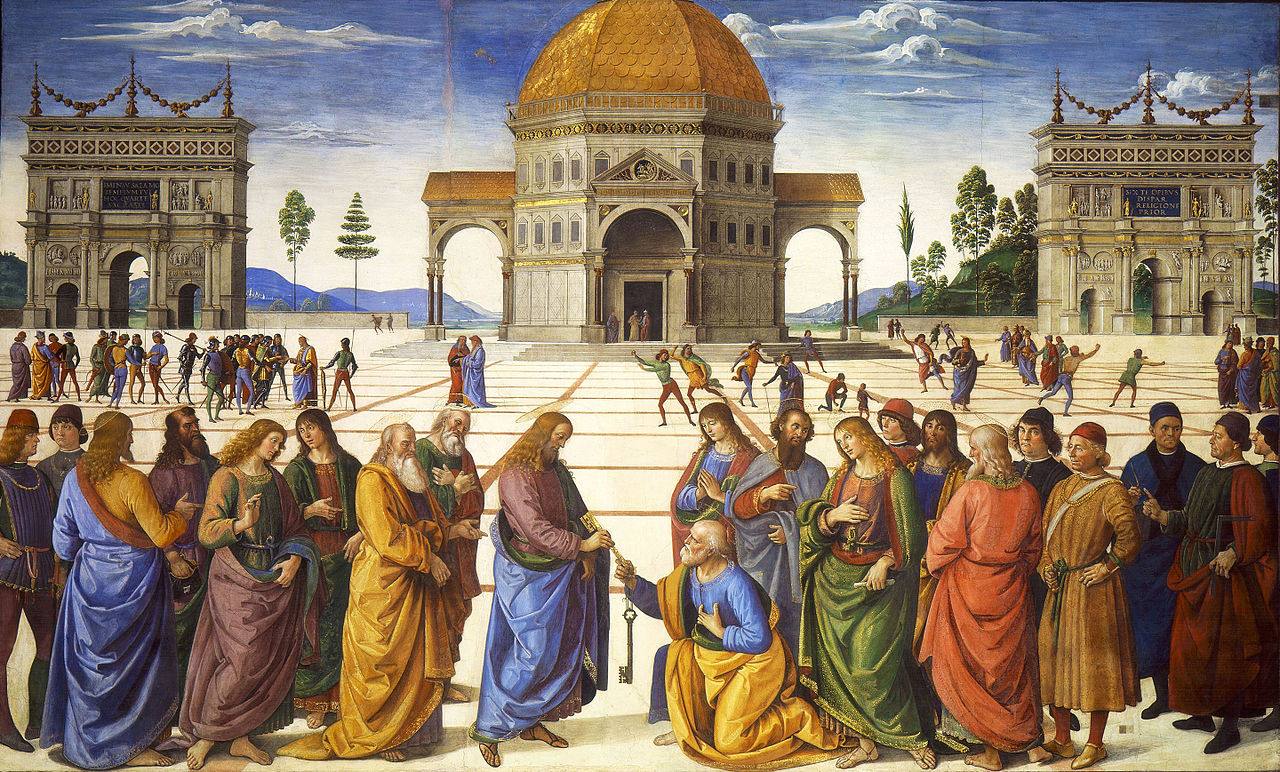
\includegraphics[width=.8\textwidth]{images/introduction/perugino.jpg}
      \end{center}
      \caption{\textit{The Delivery of the Keys}, 1481–1482, Sistine Chapel, Rome by Perugino (1481–1482). This impressive $3.3m \times 5.5m$ fresco that both illustrated linear perspective and Brunelleschi's architectural style.}
      \label{fig:intro_perugino}
\end{figure}

Even through artistic perspective studies were extremely well-tuned from a technical and mechanical standpoint \citep{simon2021jan}, perspective found new expressions in sciences few centuries later, through the advent of photogrammetry. Notion speaks for itself when we once again at its grec ethymology, \textit{photo} - \ie light -, \textit{gramma} - \ie drawing, writing - and \textit{metron} - \ie measure -. Aimé Laussedat, a French astronomer, geodesist, surveyor and cartographer used the \textit{Hôtel des Invalides} in 1849 to observe, measure and thus try to reproduce physical spaces, lines and objects from multiples perspective views. Whereas photogrammetry therefore leverages parallax effect to extract depth and dimensions from our physical world with observed views, it was intensively used during mid last century for military purposes. The advent of aerial photography, enabled by recent advancements in aviation, allowed for the topographic mapping of entire countries during the Interwar period.

\begin{figure}[h!]
      \begin{center}
      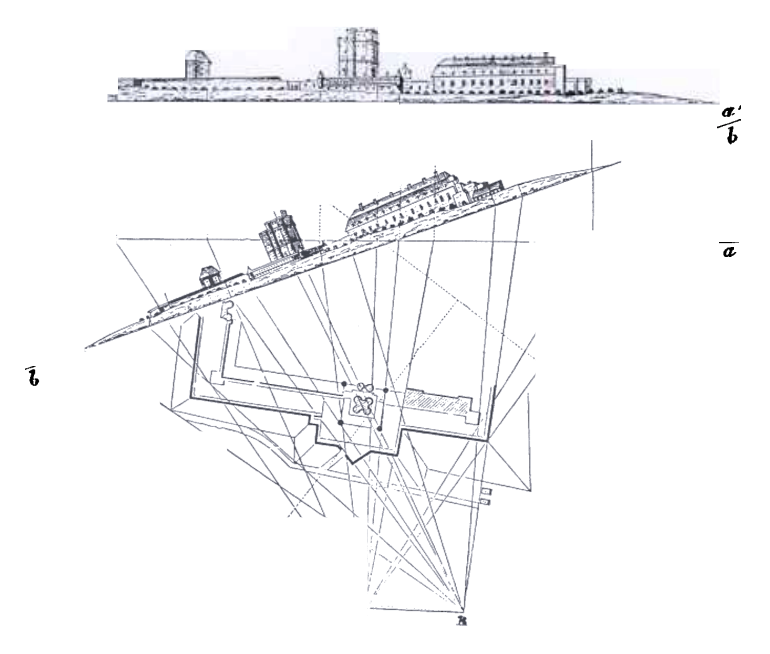
\includegraphics[width=.5\textwidth]{images/introduction/laussedat_phtograpmetrie.png}
      \end{center}
      \caption{Surveyed by the method of graphical intersections applied to perspectives recorded with the camera lucida. Survey of the Château de Vincennes by A. Laussedat, 1850}
      \label{fig:intro_laussedat}
\end{figure}

Photogrammetry has finally been heavily studied through the prism of robotics and computer vision during 1980's, with increasing computational power and emerging digital imaging technology. Structure-from-Motion approaches naturally arised from such an increasingly strong convergence between photogrammetry and computer vision in the meantime, via pioneered work from Shimon Ullman \citep{ullman1979interpretation}. Such a domain paved the way on novel view synthesis issues (and 3D reconstruction) by filling the gap between photographic scenes capturing processes and their comprehensive three-dimensional representation. 

\ac{AI}, in its commonly broad, unclear, and somewhat disputed definition within society, has a suprisingly more than a 70 years background history, with Alan Turning as the most ackwolegded earliest founding fathers of computer science \citep{turing1950computing} and artificial intelligence with John McCarthy. \ac{AI} is defined by \href{https://www.britannica.com/technology/artificial-intelligence}{The Encyclopedia Britannica} as \textit{"the ability of a computer to perform tasks commonly associated with intelligent beings"}. In the realm of Computer Vision and Graphics, this manuscript frames in a shrinked domain of \ac{AI}, commonly refered as \ac{DL}: \ac{DNN} are thus going to be considered in a large extend in the next few pages... 

\ac{DL} has itself a pationate and outstanding past history, whose one of most recognizable figures today in vision community is Yann LeCun. He has now been working over the last 30 years on vision \ac{AI} considerations, and notably introduced \ac(CNN) \citep{lecun1998gradient}, that have been widely used in this work over the last three years, even in 2024. The release in 2009 of ImageNet \citep{deng2009imagenet}, a database of millions annotated images, and the \ac{CNN} based image-classifier AlexNet \citep{krizhevsky2012imagenet} in 2012 are unanimously seen as the \ac{DL} breaktrhought debut. Vision tasks that were tackled by such \ac{DL} algorithms quickly grows in complexity, from image generation model as \ac{GAN} \citep{goodfellow2014generative} to even novel view synthesis through image-to-image network \citep{yang2015weakly}. However, if vision 2D image-based tasks has been in a large extend studied over the last decade, adding such a third dimension to adress 3D issues with \ac{AI} is a 4/5 years old challenge that now can be embrassed thanks to the latest \ac{GPU} computing advances. 

% Papier de 1998 qui commence à parler de "learn" pour ensuite embrayer sur l'IA. 
% Parler du fait que l'IA démarre par des considérations pour des sujets 2D, classifications, puis image to image, tandis que la 3D n'est finalement réellement adressée que plus tardivement, à compter de 2020. 
% Conclure ici que cette thèse s'incrit donc dans les prémisses de ce qu'est l'IA en 3D aujourd'hui. 


\citep{mildenhall2020nerf}
\citep{voleti2024sv3d} 
\citep{trevithick2023} 



\section{PhD Context}

\subsection{Meero}
Meero is a Software-as-a-Service french startup founded in 2014 that primarily aims to provide \ac{AI}-powered visual enhancement tools and algorithms for businesses across several verticals, from real estate agencies to e-commerce and fashion industries, as well as automotive car dealerships. Meero proposes a wide range of \ac{AI}-based solutions, from sky replacement, virtual staging or object eraser algorithms for the real-estate vertical to background removal or virtual try-on for fashion and e-commerce companies. Regarding its automotive branch, brand as \textit{CarCutter}, Meero offers car dealerships and marketplaces the opportunity to have visually coherent and appealing images. One of its latest product refers as the 360\degree spin, that allow to virtually smoothly turn around a car given a limited set of images. Such a 3D-based application is inherantly covered by \ac{NVS} as soon as unseen viewpoint must be rendered. 

However, fundamental research in computer vision and its conterpart application in industries suffers from a massive gap that needs to be closed: most of academic papers in vision research deal with images that roughly size from $128\times128$ to $1024\times1024$, whereas images from any mobile device now has at least a 2K resolution (up to 4 to 6K for the latest DSLR camera). Even through such claim tends to thin out with latest fundation models and exploding \ac{GPU} compute capabilities, such an image resolution discrepancy prevent, during this thesis, to directly build an image-based \ac{AI} product in industy from an academic vision paper. This thesis somehow tried to filled this gap, mostly by investigating generalizable single-image novel view synthesis architecture, that could thus be non-restricted to a single scene. 

\subsection{3D reconstruction}
 \ac{NVS} is somehow inherently intertwined with 3D reconstruction, as synthesis of novel views was, de facto, allowed when the complete 3D representation of the scene was available. While an impressive variety of approaches exists for addressing this issue; from photogrammetry-based or Structure-From-X techniques (where X could stands for \textit{Texture, Shading, Silhouette} etc) to structured-lights ones, pionner work in such area get considerations for stereo vision \citep{marr1976cooperative} via an iterative cooperative algorithm between two views. 

\subsection{Novel View Synthesis}
From very early attempt to perfrom single-image novel view synthesis in 1998 "The example images are used to "learn" a pose-invariant shape and texture description of a new face"  \cite{vetter1998synthesis} through mostly graphics and \citep{trevithick2023} 




\section{Contributions}
Aiming to perform novel viewpoint synthesis from a single-image is an extremely ill posed-problem since too many details, structures or texture are unobserved on the provided source view. Core problem that thus inherantly rises from the later observation is to find ways, such as efficient pose encoding, structural constraints that bring as many as possible prior information to the \ac{NN}. 

Years before 2023 emergence of \ac{GenAI} and incredibly powerful foundation models \citep{awais2023foundational}, dataset images we dealt with in single-image \ac{NVS} were mostly low resolution, size $128\times128$, as in ShapeNet \citep{ShapeNet}. We tried through this thesis to incorporate, as much as we possibly could, epipolar geometrical constraints and concepts. We were convinced by the same guiding principle for the last three years: \textit{the most fundamental 3D geometric considerations such as epipolar geometry must be explicitly integrated into deep neural networks.}

We tackle the \ac{NVS} problem with several approaches during this thesis, that could be summarized as follow.
\begin{itemize}
      \item \autoref{chapter:epipolarnvs}: \nameref{chapter:epipolarnvs}\\
            We start approaching single-image \ac{NVS} through the prism of camera transformation encoding. Such an information is vital for any \ac{NN} that performs \ac{NVS}, and its integration as a apriori information is far from being trivial. While several approaches exist to feed such intrinsic and extrinsic parameters to a network, we present in this chapter a novel method to encode such a camera transformation, by extensively leveraging on epipolar geometry. The work in this chapter has led to the following conference publication:
            \begin{itemize}
                \item \fullcite{landreau2022epipolarnvs}
            \end{itemize}


      \item \autoref{chapter:epinerf}: \nameref{chapter:epinerf}\\
            We then turn from camera pose encoding to inner 3D constraints consideration in \ac{NeRF}. However, we maintain the epipolar geometry concept in our work and build a feature-based attention mechanism thanks to \ac{NeRF}-based additional network, called \textit{NeRFeature}. Such a mecanism is direclty involved at training time, while we \textit{do not} have access to the target view to build epipolar constraints. Our work is currently in submission:
            \begin{itemize}
                  \item \fullcite{landreau2024epinerf}
            \end{itemize}

      \item \autoref{chapter:gausssplat}: \nameref{chapter:gausssplat}\\
            We finally relaxed the main hypothesis we dealt with in these first two apparoches to work with \ac{NVS} in a multiple-images scenario with 3D \ac{GS}. Such work mostly rely on \textit{CarCutter} 
industrial considerations, as the next generation of the current 360\degree spin stabilization. However, if rendering at training locations goes fine, stabilizing camera path to render unobserved viewpoint, and thus create seamless 360\degree car animation. 
\end{itemize}

\cleardoublepage

\acresetall % flush acronyms so they are redefined completly when first used
\chapter{Related Work}
\label{chapter:related}

% \minitoc


\chapterwithfigures{\nameref*{chapter:related}}
\chapterwithtables{\nameref*{chapter:related}}

\ifthenelse{\boolean{skipRelated}}{\endinput}{}
We give in this chapter a first overview of neural networks as well as neural radiance fields before delving into ... 

\section{Neural Network Learning}

A \ac{NN} can be defined trough 
\section{Neural Radiance Fields}

\subsection{3D reprensentation}\label{section:chapter1_3Drepresentation}

\paragraph{Implicit formulation}

\cleardoublepage
\let\leftmark=\oldleftmark


\acresetall
\chapter{Encode camera pose information through epipolar considerations}
\label{chapter:epipolarnvs}

%\newcommand{\mcL}{\mathcal{L}} \newcommand{\vx}{\mathbf{x}} \newcommand{\vh}{\mathbf{h}}
%\newcommand{\vy}{\mathbf{y}}
\newcommand{\tableindent}{\,\,\,\,}
\newcommand{\vt}{\mathbf{t}}
%\newcommand{\vyh}{\hat\vy}
\newcommand{\std}{$\pm\,$}
\newcommand{\clf}{\textit{clf}} \newcommand{\gray}[1]{{\color{darkgray}#1}}





% \begin{chapabstract}
%     abstract

% \end{chapabstract}
% \newpage

% \minitoc

\chapterwithfigures{\nameref*{chapter:epipolarnvs}}
\chapterwithtables{\nameref*{chapter:epipolarnvs}}

\ifthenelse{\boolean{skipEpipolarNVS}}{\endinput}{}


\paragraph{GAN Inversion} 

\section{MAGEC Inversion}
\label{section:magec}


\section{Introduction}

Synthesise a novel and realistic image from another viewpoint based on single or multiple images and some camera pose information commonly referred to as novel view synthesis. It has tremendous applications, from a pure computer vision and graphics perspective (such as cinemagraph, video stabilisation or 3D-based virtual staging) to \ac{AR} and \ac{VR}.

This problem can be addressed from different perspectives, depending on the available data: multiple source images, depth maps, 3D labels such as 3D scene point cloud, accurate or jittered camera poses etc. We considered in this work one of the most extreme cases for the novel-view synthesis issue. Our work constrains the prediction of a scene from a novel viewpoint by solely leveraging a single source image and the corresponding camera viewpoint transformation. 

Currently, efforts are oriented toward getting the most visually appealing results on novel view synthesis, mainly through NeRF-based methods \citep{mildenhall2021nerf,wang2021neus,barron2021mip,barron2022mip}. However, only a few works pursue another tricky challenge in the novel-view synthesis: investigating the most efficient way to condition an NVS architecture on camera pose information. From a general perspective, single-image novel-view methods often restrict the viewpoint transformation to the extrinsic matrices. Intrinsic is thus discarded since most methods around single-image novel-view synthesis ignore physical image formation properties and do not account for rendering, epipolar geometry or homography concepts. Such camera pose conditioning task remains too weakly addressed in the current literature, which motivated us to tackle such an issue elegantly.

While one of the most straightforward solutions to do so consists in encoding the relative camera viewpoint transformation as a feature vector, we claim such a method is sub-optimal, supported by one of the latest state-of-the-art works in monocular depth prediction \citep{zhao2021camera}. We thus propose in this work an elegant solution to encode the camera relative transformation as a 2D feature RGB image, by leveraging epipolar constraints. The new and implicitly encoded camera viewpoint transformation has a similar spatial resolution as the source image, somehow filling the dimensional gap between pose matrices and the RGB space. The contribution we propose in this paper is thus three-fold: 
\begin{itemize}
	\item A strategy to encode the camera pose transformation into an implicit feature image builds upon epipolar geometry considerations. 
	\item A neural network architecture which leverages such camera viewpoint transformation encoding. 
	\item A spectral loss function that extensively accounts for the higher frequencies of an image to better retrieve tiny and complex details.
\end{itemize}

\section{Related work}

\noindent\textbf{Novel view synthesis in a large extent.} Since modalities involved in novel-view synthesis are broad (images, video sequence, 3D point clouds, depth and disparity maps, camera poses), tremendous approaches investigated ways to tackle such issues. One of the latest trends takes advantage of \ac{NeRF} \citep{mildenhall2021nerf} and their incredible powerfulness to generate highly realistic scenes from unseen viewpoints \citep{wang2021neus,niemeyer2022regnerf,barron2022mip}. However, such architectures are somehow over-fitted over a unique scene and do not have any generalisation abilities. Such a drawback is growingly overcome by recent works \citep{yu2021pixelnerf,li2021mine} that tackle novel view synthesis through the prism of NeRF-based architectures. While MINE \citep{li2021mine} is a \ac{MPI} based method that requires accurate ground truth disparity maps, PixelNeRF \citep{yu2021pixelnerf} works with several input views to refine the predicted novel view. Another important line of work in novel view synthesis for indoor navigation, with datasets such as RealEstate10K \citep{zhou2018stereo} or Matterport3D \citep{zhao2021camera}, produces extremely appealing results with complex architectures \citep{wiles2020synsin,rombach2021geometry,rockwell2021pixelsynth}, often at the expense of complex information to get, such as ground truth depth maps or dense 3D point clouds. \newline

\noindent\textbf{Camera pose encoding.} Camera pose is compactly represented through: 3 degrees of rotations around each world axis, 3 other ones for translation (both defining the extrinsic matrix) and a few additional ones when intrinsic must be considered (focal length, sensor size etc). One of the most straightforward solutions encodes the viewpoint transformation by computing camera poses difference \citep{sun2018multiview}. Another pose encoding strategy embeds such a low-dimensional camera pose into a higher space, as in \citep{kim2020novel,rombach2021geometry}. These last two possibilities can be simplified if one wants to consider one-hot vectors for camera pose encoding. Finally, the closest work to ours regarding camera pose encoding is \citep{zhao2021camera}, which encodes the camera location (parametrized through a roll and pitch angles as well as a fixed height above a ground plane) as a 2D feature image for depth maps prediction purpose. \newline

\noindent\textbf{Camera pose conditioning.} Extrinsic camera pose is thus often the unique 3D prior information that conditions the neural network for generating a novel view. Based on the camera pose difference $P_{diff}=P_{target}-P_{source}\in \mathbb{R}^{v}$, the authors from \citep{sun2018multiview} tiled such vector across all the pixels of the source RGB image, feeding their CNN-based architecture with inputs that size $\mathbb{R}^{H\times W\times (3+v)}$. On the other hand, \citep{kim2020novel} adopts a different strategy and concatenates its camera pose feature vector with the one obtained from their CNN-encoder before feeding it to the decoder. 
Finally, \citep{wiles2020synsin} designed a single image novel-view synthesis method that extensively relies on 3D point cloud consideration. Camera viewpoint transformation is used within the network architecture to update the predicted point cloud before rendering. \newline

\noindent\textbf{Single-image novel view synthesis.} Such a framework is the most challenging one since only minimal information is available during training and inference: a source image and a corresponding camera pose transformation that accounts for the target image we aim to generate. To the best of our knowledge, only a few recent works \citep{sun2018multiview,kim2020novel,yu2021pixelnerf}  deal with such a highly constrained setting. While \citep{sun2018multiview, kim2020novel} both handle "discrete" (from ShapeNet \citep{chang2015shapenet}, parametrized through a unique azimuthal angle, the elevation one being fixed) and continuous (as in Synthia \citep{ros2016synthia} and KITTI \citep{geiger2012we}) camera transformations, the pose-feature vector needs to be updated accordingly from a size perspective. This is one of the main benefits of the method we designed. Both discrete and continuous camera information is encoded through a featured image that sizes the same as the source image and that truly leverages the real-world camera transformation that occurred between the source and the target view. Such convenient property allows to inferring (at least with discrete camera poses) viewpoints that were not represented within the training set. \newline

\section{Method}
\subsection{Camera viewpoint transformation encoding}
\subsubsection{Epipolar geometry overview }

The general framing of our work might be considered one of the trickiest ones in novel-view synthesis since the image generation from a different camera viewpoint is only made prior to a single source image and a relative camera transformation. 

We denote by $I_{s} \in \mathbb{R}^{H\times W\times 3}$ the RGB source image and $I_{t}$ the target one we aim to predict.
The pinhole convenient camera model that we get consideration for is represented through an intrinsic matrix $K \in \mathbb{R}^{3\times3}$. The rigid motion that accounts for the relative transformation between the source and the target view consists of a rotation $R \in SO(3)$ and translation $T\in \mathbb{R}^{3\times1}$, expressed through each camera's extrinsic:
\begin{equation}
     \begin{cases}
     R = R_{t} R_{s}^{T} \\
     T = t_{t} - R t_{s}
     \end{cases}
\end{equation}
with $(R_{s},t_{s})$ and $(R_{t},t_{t})$ respectively accounting for the source and target camera extrinsic. Epipolar geometry \citep{hartley2003multiple} has consideration for the projective geometry that connects two camera viewpoints and has various applications such as Structure from Motion \citep{tamaazousti2011nonlinear}. Epipolar geometry aims to describe the relationship that stands between 3D world location and 2D pixel coordinates, given a stereo pair of cameras and their corresponding poses. The fundamental matrix F is a $3\times3$ matrix that entirely describes such 3D/2D mapping and can be obtained through: 
\begin{equation}
    \mathbf{F} = K^{-T} [T]_{X} R  K^{-1}
\end{equation}

with $[.]_{X}$ the skew-symmetric matrix representation of any one-dimensional vector. Given a pixel location\footnote{Homogeneous coordinates are implicitly used here but omitted for clarity reason} $p_{s}\in I_{s}$, such fundamental matrix $\mathbf{F} \in \mathbb{R}^{3\times3}$ allows to define: 
\begin{equation}
    \mathcal{P}_{p_{s}} = \{p_{t}\in I_{t} | p_{t}^{T}\mathbf{F}p_{s} = 0 \}
\end{equation}

as the finite set of pixels from $I_{t}$ that live on the epipolar line defined by $l=\mathbf{F}p_{s}$. From a pure geometrical perspective, such line corresponds to the rendered (on $I_{t}$ camera plane) 3D ray that passed through both the camera center of $I_{s}$ and $p_{s}$. 

The fundamental matrix $\mathbf{F}$ makes a pixel-to-line correspondence through a linear equation that involves both the source and the target original camera location. As soon as we aim to use the epipolar geometry to encode the viewpoint transformation, a sampling strategy needs to be set in order to determine which pixel location from the source image $I_{s}$ are going to be used to compute these epipolar lines. Instead of randomly sampling location over the $H\times W$ possibilities, and motivated by experiments that can be found in the Supplementary, pixels are sampled according to a regular grid $\textbf{G}_{r}$ that spans the whole image, parameter \textit{r} controlling how coarse the grid is: 

\begin{equation}
    \mathbf{G}_{r} = \left\{(p_{x},p_{y}) \in \{1,..,H\}\times \{1,..,W\} \Big\rvert \begin{array}{l}
                    p_x \equiv 0 \pmod{H/r}\\
             p_y \equiv 0 \pmod{W/r}
              \end{array}\right\}
\end{equation}


\subsubsection{Encode the camera viewpoint transformation}

Our module encodes the relative camera motion it exists between the source and target views by extensively leveraging epipolar geometry. Its output is fed to one of the branches of our NVS neural network as a feature image, that thus implicitly represents the transformation that occurred, and is referred as $E_{s\xrightarrow{}t}$.
An overview of the different stages involved to compute $E_{s\xrightarrow{}t}$ is presented through the pseudo-code\footnote{Some pixel values on $E_{s\xrightarrow{}t}$ might be overwritten by another pixel $p$. We claim the sampling order over \textbf{G} has no impact on the encoding strategy.} below in Algorithm \ref{pseudoCode}. \newline

As seen in Algorithm \ref{pseudoCode}, each epipolar line reported on $E_{s\xrightarrow{}t}$ has a distinct colour, the one associated with the sampled pixel on $I_s$. Such implementation choice gives additional RGB prior information to the network regarding the colour that should be generated, even though lightning issues are not considered. One might notice that the last epipolar lines plotted on $E_{s\xrightarrow{}t}$ would overwrite some previous ones, at least at some specific pixel location (on epipoles for instance). We claim, based on experimental observations, that pixel sampling order (and thus epipolar line overwriting) does not have an impact that is significant on the training and inference performances of the model. 

The encoding method depicted here is thus able to encode any form of camera viewpoint transformation without any structural adaptation. Indeed, most concurrent works need to change the way viewpoint transformation is encoded since continuous poses are not processed the same way as discrete ones, where a one-hot encoding strategy might be used. 

\begin{algorithm}[h!]
\caption{Epipolar Encoding module \label{pseudoCode}}
\begin{algorithmic}[1]
\Procedure{Input: $(I_{s},F,\mathbf{G}_{r})$}{}
\State $E_{s\xrightarrow{}t} = \textit{zeros(H,W,3)}$
\For {$p_{G}$ in $\mathbf{G}_{r}$}
\State $colRGB=I_{s}[p_{G}]$
\State \text{Build up} $\mathcal{P}_{p_{G}}$
\State $\forall p \in \mathcal{P}_{p_{G}},\hspace{.2cm} E_{s\xrightarrow{}t}[p]=colRGB$
\EndFor
\State Return $E_{s\xrightarrow{}t}$
\EndProcedure
\end{algorithmic}
\end{algorithm}

Only non-null pixel values are sampled from $\textbf{G}_{r}$ in our encoding strategy for ShapeNet \citep{chang2015shapenet} since pixels located in the background do not bring any valuable information regarding the corresponding coloured epipolar lines. Figure \ref{fig:examplePoseEncoded} represents the kind of results one might expect with our viewpoint camera transformation encoding strategy on ShapeNet \citep{chang2015shapenet}. 
\begin{figure}[h!]

\begin{center}
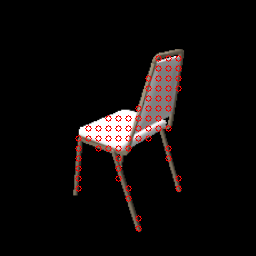
\includegraphics[width=.26\textwidth]{images/epipolarnvs/Is_ECML.png}\hspace{.5cm}%\hfill
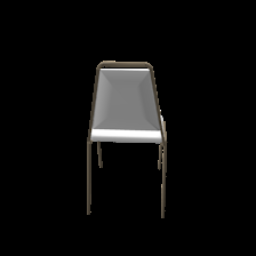
\includegraphics[width=.26\textwidth]{images/epipolarnvs/It_ECML.png}\hspace{.5cm}%\hfill
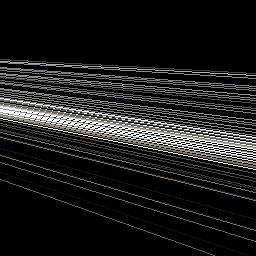
\includegraphics[width=.26\textwidth]{images/epipolarnvs/Est_ECML.jpg}
\end{center}
\caption{From left to right: Source image $I_s$, Target image $I_t$ and the corresponding $E_{s\xrightarrow{}t}$. From the ShapeNet \citep{chang2015shapenet} \textit{chair} class. Pixel locations sampled from $\textbf{G}_{25}$ are highlighted through red circles.}
\label{fig:examplePoseEncoded}
\end{figure}



\subsubsection{Extended strategy for encoding}

Performing novel view synthesis on Synthia \citep{ros2016synthia} and KITTI \citep{geiger2012we} datasets is, from a relative camera transformation perspective, somehow redundant and tricky through our encoding framework. Indeed images contained in these datasets have been recorded through a car driving across city streets, and most of the camera transformations considered are translation motions. Such viewpoint changes between the source and target views are improperly handled by the epipolar theory since depth cues are lost. We therefore extended our initial encoding strategy for those datasets through a fourth channel that primarily accounts for such depth information.

Let's denote:
\begin{equation}
    \Delta_{t}= |t_{t}| - |t_{s}| = \left[\Delta t_{X},\Delta t_{Y},\Delta t_{Z} \right]^{T} \in \mathbb{R}^3
    \label{eq:delta_t}
\end{equation}
the difference between the two absolute translations $t_s$ and $t_t$. Absolute values are taken in Equation \ref{eq:delta_t} since 2D planes coordinates are not standardised across scenes in KITTI \citep{geiger2012we} and Synthia \citep{ros2016synthia}. The meaningful scalar value of interest is referred as $\delta_{t}$ and is computed through:
 
 \begin{equation}
 \label{eq:2}
     \delta_{t} = sign(t_{M}) \times| t_{M} |
 \end{equation}
 with \newline
 \begin{equation}t_{M} = \Delta_{t}\left[p_{M}\right] \hspace{.3cm} ;  \hspace{.3cm} p_{M}=\argmax |\Delta_{t}|\end{equation}

The expression of $\delta_{t}$ satisfies two resourceful constraints in our case: 

\begin{itemize}
    \item It accounts for the main car motion direction and gives some insight regarding the distance the car moved between the source and target view.
    \item The sign of $\delta_{t}$ indicates whether the source/target frames that were sampled correspond to a forward or backward motion. 
\end{itemize}
Such properties allow the network to better apprehend the direction of the motion it should take into consideration. The value of  $\delta_{t}$ is finally stored on a fourth channel of $E_{s\xrightarrow{}t}$ only at locations where the epipolar lines had non-zero values in the first three RGB channels. 

\subsection{Network architecture and Training loss}

The overall network architecture is presented in Figure \ref{fig:architecture}. Such architecture takes inspiration through the one \citep{kim2020novel} introduced in their work, at least regarding the image-to-image U-Net based encoder/decoder structure with the hard-flow attention strategy. However, the way the transformation viewpoint information is provided to the network architecture drastically changes for our model. While \citep{kim2020novel} performed feature-vectors concatenation at the network's bottleneck stage, we claim such choice is sub-optimal, at least for discrete camera pose information as contained in ShapeNet \citep{chang2015shapenet}. We thus rather encode this camera pose transformation through $E_{s\xrightarrow{}t}$ as an image that feeds a second CNN-based encoder. This last encoder produces a feature vector that will be concatenated to the one obtained by the U-Net based encoder before being consumed by the decoder. 

\begin{figure}[h!]
  \begin{center}
  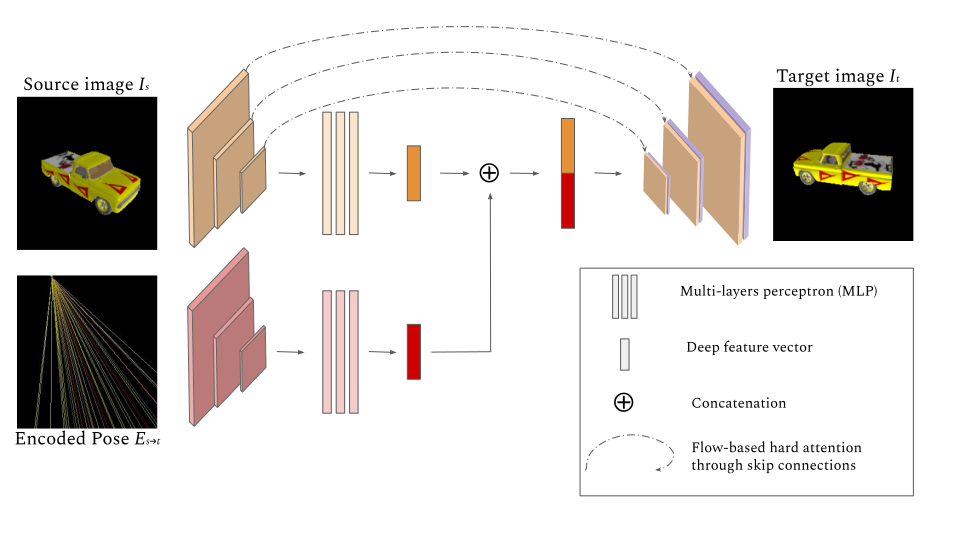
\includegraphics[width=\textwidth]{images/epipolarnvs/NetworkArchitecture.png}
  \end{center}
  \caption{General overview of our architecture. Network takes as inputs both $I_s$ and $E_{s\xrightarrow{}t}$ through two distinct encoders that produce feature vectors that are concatenated before being fed to the decoder. The network structure also leverage on the hard flow attention connections introduced in \citep{kim2020novel}.}
  \label{fig:architecture}
\end{figure}

The total loss function is a weighted sum  of a Mean Average Error (MAE) , referred as $\mathcal{L}_{1}$ and used in \citep{kim2020novel}, and a second term, called $\mathcal{L}_{spectral}$, directly inspired form prior super-resolution work \citep{fritsche2019frequency} and that extensively focuses on the preserving high frequencies. Indeed, considering a 2D Gaussian filter $w_{gauss}$, an image $I$ can be decomposed into a low and a high-frequency components, respectively noted as $I^{LF}$ and $I^{HF}$ : 
\begin{equation}
\begin{cases}
     I^{LF}  = I\circledast w_{gauss} \\
     I^{HF} = I - I^{LF} = (\delta - w_{gauss})\circledast I
\end{cases}
\end{equation}
where $\circledast$ represents a 2D convolution operation. 
The final loss function used during training is thus given by: 
\begin{equation}
    \mathcal{L} = \mathcal{L}_{1} + \lambda \mathcal{L}_{spectral} = |\hat{I}_{t} - I_{t}| + \lambda \left( \hat{I}_{t}^{HF} - I_{t}^{HF} \right)^{2}
    \label{eq:1}
\end{equation}



Additional details on $\mathcal{L}_{spectral}$ are available in the Supplementary.

\section{Experiments}
All qualitative and quantitative results we obtained through our camera pose encoding strategy are presented in this section. \newline

\noindent\textbf{Datasets.} We experimented our method on the same dataset as \citep{kim2020novel, sun2018multiview}: on the \textit{chair} and \textit{car} class from ShapeNet \citep{chang2015shapenet} as well as on real scene images from KITTI \citep{geiger2012we} and Synthia \citep{ros2016synthia}.
Results we reported for \citep{kim2020novel} slightly differ from the ones published since we get consideration for a more challenging rendering scenario: jittered camera pose in ShapeNet \citep{chang2015shapenet}, elements on image borders from Synthia \citep{ros2016synthia} and KITTI \citep{geiger2012we} are not removed anymore through  center-cropping , etc. Such changes are motivated and fully exposed in the Supplementary.  \newline

\noindent\textbf{Training - Testing.} We trained our model on 100,000 iterations, using the same training procedure as \citep{kim2020novel}. Since our camera pose encoding strategy is light enough, we perform ``on the fly'' batch creation during training. Inference scores were averaged over 100 runs with batch sizes of 16. \newline


\noindent\textbf{Metrics.} We used the \ac{MAE},  \ac{SSIM} \citep{wang2004image} and \ac{PSNR} metrics to score our novel view synthesis architecture. 

\subsection{Qualitative Results}

We present in Figure \ref{fig:res_all} an instance of all the datasets we get consideration for. Whereas our model manages to infer and reason about the object size according to the target view on the \textit{Car} and \textit{Chair} classes, novel-view produced by \citep{kim2020novel} fails to do so, producing a result that rather roughly matches the source object size. Our results on these two classes are also sharper and more realistic, both from colour and geometrical perspectives. The car's wheels or the chair's complex back are thus better synthesise with our method. 

Because \citep{kim2020novel} integrates the camera pose as discretized bins, the viewpoint transformation loses its physical inner 3D consistency structure. On the other hand, our method produces an encoding that fully accounts for the continuous pose transformation that occurred.\newline


\begin{figure*}[h!]
    \begin{center}
    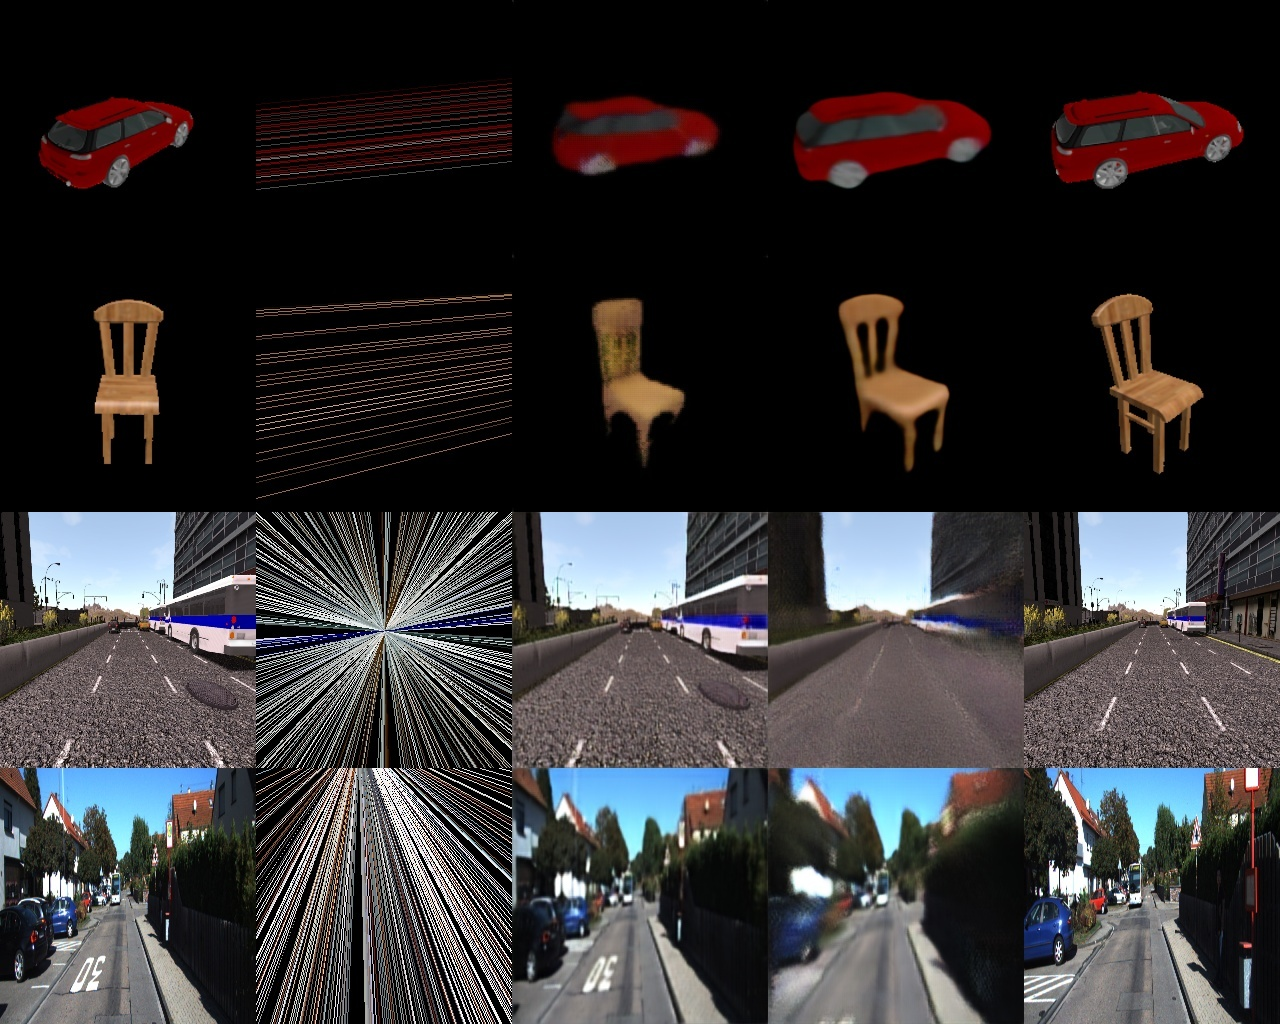
\includegraphics[width=.8\textwidth]{images/epipolarnvs/resultsFinal_BMVC.jpg}
    \end{center}
     \caption{Inference results on all the four datasets considered. $E_{s\xrightarrow{}t}$ encoded transformation have been obtained with $\textbf{G}_{15}$. From left to right: the source image  $I_s$, $E_{s\xrightarrow{}t}$, \citep{kim2020novel} prediction, our prediction, the target image $I_t$. On overall, our method predicts more consistent results since complete pose transformation has been fed to the network contrary to the concurrent work from \citep{kim2020novel}. }
     \label{fig:res_all}
\end{figure*}

Results of our method synthesised on real-world datasets are depicted on third (Synthia \citep{ros2016synthia}) and fourth (KITTI \citep{geiger2012we}) rows of the Figure \ref{fig:res_all}. One might noticed how the car moved between the source and the target view in the Synthia \citep{ros2016synthia} dataset. While our results remain blurry, our network architecture successfully hallucinated the forward motion that the bus had. On the other hand, our main concurrent work mostly predicts the source image, and fails to capture the relative displacement that occurred in this example. An almost similar scenario is inspected on KITTI \citep{geiger2012we}. While the sign "30" on the ground has disappeared between the two views, our method successfully captures such drastic change while \citep{kim2020novel} fails to the same extent as previously. We emphasise the fundamental role our camera encoding strategy has here, especially regarding the shape of the various objects where the perspective changes a lot between $I_s$ and $I_t$ (on the roof of the house, top left border). \newline


While results presented on Figure \ref{fig:res_all} for real world datasets focus on the overall motion that occurred, we highlight on Figure \ref{fig:res_all2} in which extent high-frequency details can be retrieved by our model. The global motion is quite properly handled by \citep{kim2020novel} too, but our method manages to better retrieved tiny details structure for the paintings on the ground. The Spectral loss we used during training helped the network to handle these high frequencies. A complete ablation study regarding the impact the Spectral loss has can be found in the Supplementary, in addition to several other visual results on the four datasets we considered.
\begin{figure*}[h!]
    \begin{center}
    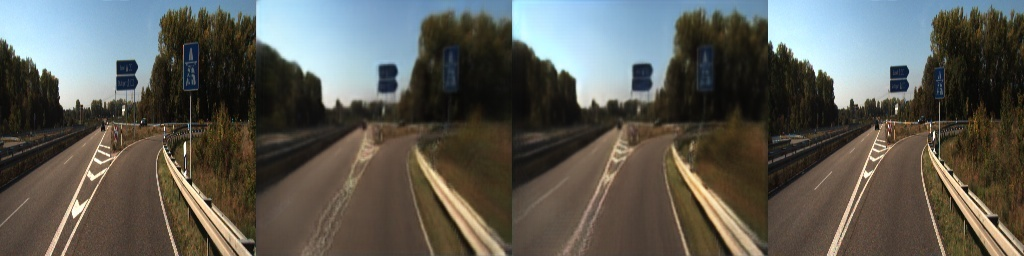
\includegraphics[width=.8\textwidth]{images/epipolarnvs/rebbutal_KITTI_3.jpg}
    \end{center}
     \caption{From left to right: the source image  $I_s$, \citep{kim2020novel} prediction, our prediction, the target image $I_t$. Painting on the ground are better reconstructed in our method compared to \citep{kim2020novel}.}
     \label{fig:res_all2}
\end{figure*}

  
\subsection{Quantitative Results }

We report some performance results over the four datasets we get consideration for. Tables \ref{tab:1} and \ref{tab:2} respectively summarise the scores for the synthetic ShapeNet \citep{chang2015shapenet} dataset and the real-scene ones (Synthia \citep{ros2016synthia} and KITTI \citep{geiger2012we}). While our method outperforms concurrent works on MAE, we reach extremely competitive results with the SSIM metric too, since only \citep{sun2018multiview} gets better scores. \newline

However, we emphasise on a crucial aspect regarding the reported scores. Only our method and the one from \citep{kim2020novel} has been retrained with the extended and challenging datasets that we presented earlier. Results from remaining works \citep{tatarchenko2015single,zhou2016view,park2017transformation,sun2018multiview,} are the ones that were originally published by authors. 
\begin{table}[htp!]
\begin{center}
\begin{adjustbox}{max width=\textwidth}
\begin{tabular}[h]{c||ccccccc}
\hline
Modality & Method & \multicolumn{3}{c}{Car} & \multicolumn{3}{c}{Chair} \\
 & & $MAE$ ($\downarrow$) & SSIM ($\uparrow$) & PSNR ($\uparrow$) & $MAE$ ($\downarrow$) & SSIM ($\uparrow$)) & PSNR ($\uparrow$) \\
\hline
\textit{Multi-views} &\citep{sun2018multiview} & $0.078$ & ${0.935}$ & - & $0.141$ & ${0.911}$ & -\\
\hline
& \citep{tatarchenko2015single} & $0.139$ & $0.875$ & - & $0.223$ & $0.882$ & -\\
&\citep{zhou2016view} & $0.148$ & $0.877$ & - & $0.229$ & $0.871$ & - \\
\textit{Single-view} &\citep{park2017transformation} & $0.119$ & $\underline{0.913}$ & - & $0.202$ & 0.889& -\\
& \citep{yu2021pixelnerf} & - & 0.900 & \underline{23.17} & - & $\mathbf{0.911}$ & $\mathbf{23.72}$ \\
&\citep{kim2020novel} & $\underline{0.026}$ & $0.892$ & 21.18 & $\underline{0.045}$ & $0.865$ & 17.89\\
& Ours & $\mathbf{0.016}$ & $\mathbf{0.928}$ & $\mathbf{24.23}$ & $\mathbf{0.032}$ & \underline{0.901}& \underline{19.55}\\
\hline \hline

\end{tabular}
\end{adjustbox}
\end{center}
\captionof{table}{Performance on ShapeNet \citep{Shapenet}. Best scores for the single-view modality are highlighted in bold while second best ones are underlined.}
\label{tab:1}
\end{table}

 Results on Synthia\citep{ros2016synthia} and KITTI \citep{geiger2012we} are reported on Table \ref{tab:2} and are competitive with current state of the art methods. We emphasize that our method (as well as \citep{kim2020novel}) was trained on more complex scenarios from an image-content perspective: both Synthia and KITTI images were resized to $256\times 256$ without any center-cropping operation (which allows to discard the most challenging elements from the scenes). 

\begin{table}[htp!]
\begin{center}
\begin{adjustbox}{max width=\textwidth}
\begin{tabular}[h]{c||ccccccc}
\hline
Modality &Method & \multicolumn{3}{c}{Synthia} & \multicolumn{3}{c}{KITTI} \\
& & $MAE$ ($\downarrow$) & SSIM ($\uparrow$)& PNSR ($\uparrow$) & $MAE$ ($\downarrow$) & SSIM ($\uparrow$) & PNSR ($\uparrow$)\\
\hline
\textit{Multi-views}&\citep{sun2018multiview} & $0.118$ & $0.737$ & - &  $0.163$ & $0.691$ & - \\
\hline
&\citep{tatarchenko2015single} & $0.175$ & $0.612$ & - &  $0.295$ & $0.505$ &  - \\
\textit{Single-view} & \citep{zhou2016view} & $0.221$ & $\mathbf{0.636}$ & -  & $0.418$ & $0.504$ & - \\
 & \citep{kim2020novel}  & $\underline{0.065}$ & $\underline{0.632}$ & $\mathbf{19.81}$ & $\underline{0.087}$ & $\underline{0.602}$ & \underline{16.84} \\
& Ours & $\mathbf{0.065}$ & $0.631$ & \underline{19.44} & $\mathbf{0.082}$ & $\mathbf{0.609}$ & $\mathbf{17.11}$ \\
\hline\hline
\end{tabular}
\end{adjustbox}
\end{center}
\captionof{table}{Performance on Synthia \citep{ros2016synthia} and KITTI \citep{geiger2012we}. Best scores for the single-view modality are highlighted in bold while second best ones are underlined.}
\label{tab:2}
\end{table}


\section{Limitations and further works}
The pose encoding strategy introduced in this paper is an innovative and elegant solution to integrate the camera pose transformation in the novel view synthesis issue. However, our method suffers from some limitations that might be tackled to reach even better results, both from image quality and timely processing perspectives. Indeed, since we compute the encoded viewpoint transformation $E_{s\xrightarrow{}t}$ "on the fly" during training, our method is slower than our main concurrent work \citep{kim2020novel}. Another further line of work concerns the camera data requirements that could be more flexible since one might argue that our method requires intrinsic parameters in addition to the extrinsic ones. 

One might finally also think for future work about leveraging onto the encoded relative poses we designed to better constraints the network during training through a cyclic loss function. Indeed, it would be possible to define a reversed encoded relative pose through $E_{t\xrightarrow{}s}$, by leveraging the predicted novel view. 
\subsection{Methodology}
 
\noindent \textbf{GAN-Inversion Framework} Given a 


 \subsection{Experimental Setup for Car edits}

 \minipar{Datasets and Evaluation Editors}
 
\minipar{Pretrained GAN Model}


\minipar{Training Configurations} 

\section{Conclusion}
In this paper, we proposed a new and innovative method to encode the camera transformation for the deep learning-based novel view synthesis task. For this, we leverage epipolar geometry in order to encode such viewpoint displacement as an image that we call the encoded relative pose $E_{s\xrightarrow{}t}$ (made of several coloured epipolar lines). We argue this new camera transformation encoding is better suited for the single-image novel view synthesis issue than the standard way that only consists in considering the extrinsic values of the camera transformation. Indeed, the idea behind the vanilla approach is to feed the neural network with an RGB source image and a camera viewpoint transformation to generate a new image that can be viewed as the impact of such displacement on the input image. Our method rather proposes to provide both an RGB source image and the encoded image of the viewpoint transformation, which is already a strong insight into the impact of the displacement on this image. In other words, the core motivation of our proposed method is to help the network to better understand the correlation between the input image and the desired camera viewpoint transformation. The experimental results on the different datasets presented in this work confirm our claim. These results tend to prove that this new encoding strategy is more robust to complex displacements, namely large perspective changes and also generates images with sharper details. 
\cleardoublepage
\let\leftmark=\oldleftmark

\acresetall
\chapter{Epipolar Attention in NeRF}
\label{chapter:epinerf}


\chapterwithfigures{\nameref*{chapter:epinerf}}
\chapterwithtables{\nameref*{chapter:epinerf}}

\ifthenelse{\boolean{skipEpiNeRF}}{\endinput}{}


\section{Introduction}


Few-shot NVS presents a challenging task in computer vision, wherein the objective is to generate an image from an unobserved viewpoint using only a limited number of source images and their corresponding camera pose information. The present work addresses an even more intricate scenario, which exclusively relies on a unique source image. The problem is inherently ill-posed as a single source image may not provide enough visual clues to generate a novel viewpoint. Handling unforeseen elements as well as occlusions becomes particularly challenging in this scenario. To effectively tackle these challenges, leveraging 3D priors \citep{saito2019pifu,johari2022geonerf} is fundamental since it enables deep architectures to acquire a primary understanding of the underlying 3D scene structure. 

Recent advances in neural rendering \citep{tewari2022advances} significantly drive latest works in the few shot NVS issue. While original neural radiance field (NeRF) \citep{mildenhall2020nerf} allows to represent a scene through a learned overfitted 5D function, it does not have any generalization abilities. Latest contributions \citep{yu2021pixelnerf,li2022symmnerf,lin2023vision} designed low-resolution 2D feature \textbf{F} conditioning to tackle such a limitation, mostly by leveraging on an image encoder. Produced feature volume is sampled at training and testing time through pixel-aligned bilinear interpolation to \textit{locally} condition the radiance field. However, the deep feature is aligned with the source view: occlusions and unobserved parts therefore lead to misaligned and coarsely-local feature sampling on \textbf{F}, producing non-optimal conditioning. 

\begin{figure}[htp!]
    \center
  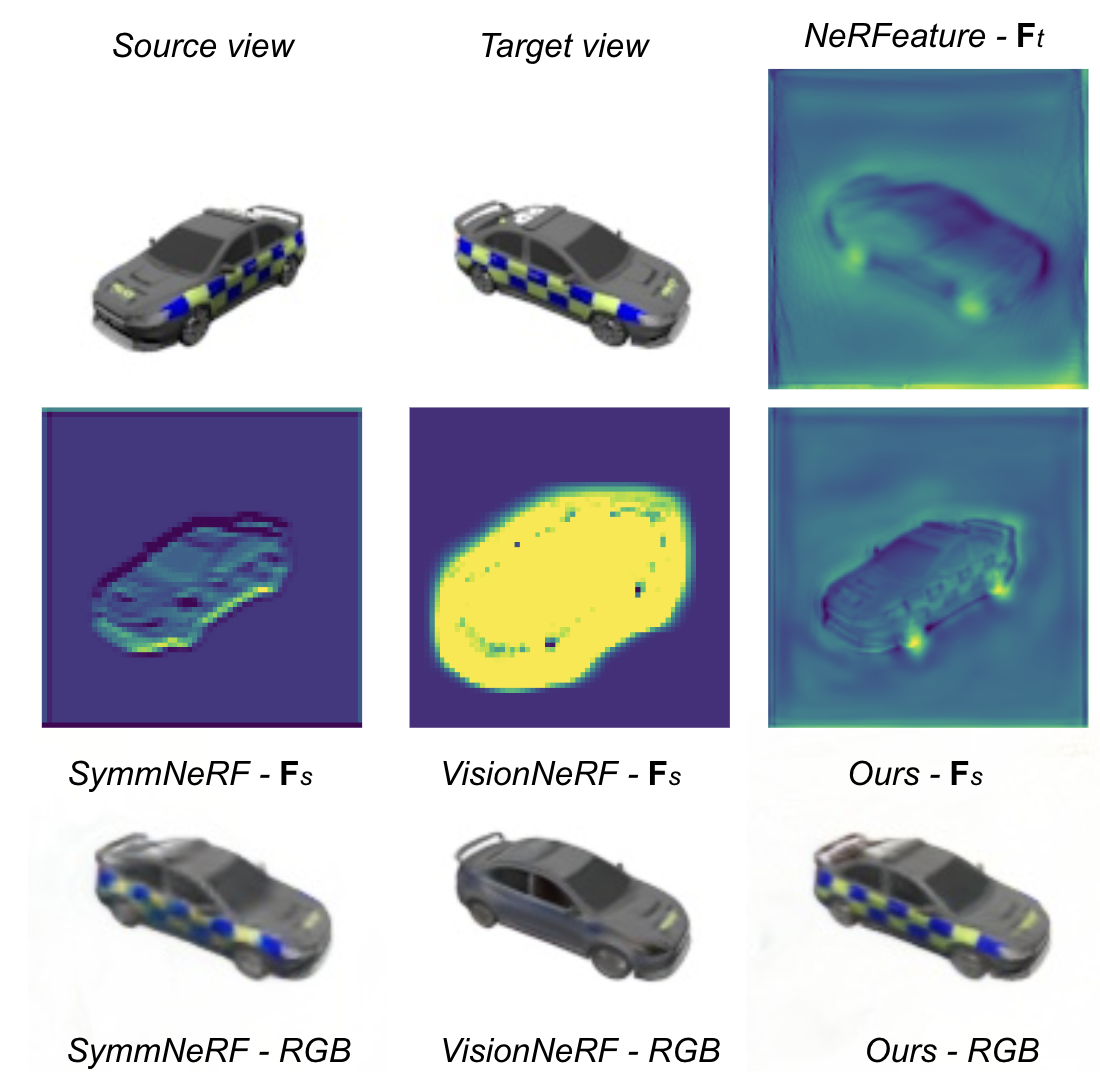
\includegraphics[width=.65\textwidth]{images/epinerf/abstract_figure.png}
  \caption{Comparison with state-of-the-art methods, both in RGB space as well as on feature space. Existing methods rely only on source-aligned features. In contrast, the proposed method uses both a source and a target-aligned features to predict the image associated to the target view, leading to a better quality rendering. In this example, VisionNeRF \citep{lin2023vision} correctly synthesised the rear wing, but fails to render the yellow and blue checkerboard painted on both car' sides. If SymmNeRF \citep{li2022symmnerf} manages to reproduce such a pattern, it lacks details on the rear wing too.}
  \label{fig:res_car_intro}
\end{figure}

Our work therefore try to address such limitations by producing target-aligned features from a feature radiance field, called NeRFeature. Associated training is supported through a light feature distillation procedure, by leveraging on a CNN encoder-decoder as teacher network. Target oriented feature (from the NeRFeature student radiance field) is then involved (with its source-aligned counterpart) in an epipolar-based attention mechanism: it shrinks the weights sampling distribution around regions where source and target features match, allowing better sampling during neural rendering. Corresponding results, both in RGB and feature space can is illustrated on Figure \ref{fig:res_car_intro}. We conducted extensive ex\--periments and ablations studies to motivate our claims, whereas our architecture outperforms most of current state-of-the art methods on the ShapeNet dataset \citep{chang2015shapenet}. Our contributions are threefold and can be summarised through: 
\begin{enumerate}
   \item A learned feature radiance field, called NeRFeature. Given a source-aligned feature and a camera transformation, NeRFeature aims to infer the correspond\--ing target-aligned deep feature trough a light feature distillation procedure, that do not involve any heavy foundation models (section \ref{subsec:nerfeature}). 
    \item A simple yet effective epipolar-based attention mechanism that relies on source and target aligned features and which adjust the weights sampling distribution during volume rendering (section \ref{subsec:epipolar_att}). 
    \item A novel generalizable NeRF architecture for single-image NVS, EpiNeRF, \textit{locally} conditioned on its input with a CNN as well as \textit{globally} conditioned on its weights through a Hypernetwork (section \ref{subsec:epinerf}).  
\end{enumerate}

\section{Related work}

\noindent\textbf{Single-image novel view synthesis.} Novel view synthesis aims to render an image of a scene from a an unobserved viewpoint, given a set of posed images, i.e. images and the associated camera poses (3D position and orientation). NVS has been widely studied over the last few decades from both graphics and computer vision perspectives. Early pioneer works \citep{chen93view,levoy96light,fitzgibbon2005image} mostly relied on graphics and multi-view geometry concepts, such as light field, warping or blending operations to synthesise novel view. However, synthesising a viewpoint from a different location based on a single image is an ill-posed task. Occluded parts cannot be easily recovered in this scenario, as the 3D scene cannot be triangulated. The recent breakthrough of deep networks has opened the door for learning-based methods. While fully convolutional-based networks first appeared in the devoted literature \citep{zhou2016view,sun2018multi,kim2020novel,hou2021novel,guo2022fast,landreau2022epipolarnvs}, the emergence of neural radiance fields \citep{mildenhall2020nerf} and neural rendering \citep{tewari2022advances} highly influenced the way single-view novel view synthesis architectures \citep{yu2021pixelnerf,li2022symmnerf,lin2023vision} are built. Introducing explicit 3D concepts (regarding camera pose, implicit or neural 3D reasoning etc) within architectures significantly help deep neural networks to better address such 3D vision task relying on implicit representations. Latest research directions in single-image NVS pushes toward extremely large deep networks, such as image-conditioned diffusion models\citep{chen2023single,xiong2023light,chan2023genvs,yu2023long}. Note that, recent advances in large 3D reconstruction \citep{hong2023lrm} use even bigger models, that are able to explicitly grasp the whole 3D structure of an object from a single view \citep{liu2023zero,shi2023zero123++,liu2024one,liu2023one2345++,zou2023triplane}. However, these diffusion-based architectures remain complex to train and have poor speed inference performances.  

\noindent\textbf{3D Geometry prior in single-image NVS.} Few works attempted to integrate geometrical priors within their single-image NVS architecture. Whereas Epipolar\--NVS \citep{landreau2022epipolarnvs} directly incorporates the geometrical camera transformation through a finite set of epipolar lines, SymmNeRF \citep{li2022symmnerf} integrates a symmetrical constraint with a simple yet effective assumption in the canonical coordinates system. 
\newline

\noindent\textbf{Generalizable NeRF conditioning.} Introduced in Mildenhall's \etal \citep{mildenhall2020nerf} work, a neural radiance field $\psi$ aims to implicitly represent the inherent geometry and appearance of a scene. In its original formulation, a set of posed images $\{I,\pi = K[R|t]\}$ is sufficient to learn such a radiance field. Given a 3D point in world space $\mathbf{x} \in \mathbb{R}^{3}$ along a ray and its viewing direction $\mathbf{d} \in \mathbb{R}^{3}$, a vanilla RGB radiance field is entirely defined through its density $\sigma_{\psi}(\mathbf{x})\in \mathbb{R}_{+}$  and an RGB colour $c_{\psi}(\mathbf{x},\mathbf{d}) \in \mathbb{R}^{3}$. 
A differentiable volume rendering operation \citep{max1995optical} is performed to render the final composite RGB color $\hat{c}$ along the ray. 

However, this formulation prevents $\psi$ to generalise across multiple scenes. While plethora works nowadays rely on deep feature volume to condition their neural architecture \citep{saito2019pifu,wang2021ibrnet,chen2023matchnerf}, PixelNeRF \citep{yu2021pixelnerf} has paved the way to such limitation in single-image NVS. It locally conditions its radiance field using pixel-wise source aligned features, obtained from a CNN encoder-decoder. 

Such a $d_{\text{feat}}$-dimensional pixel-aligned feature is obtained through the perspective projection of a 3D point onto the  source-aligned feature volume.

\begin{equation}
    c_{\psi} \colon \mathbb{R}^{3}\times\mathbb{R}^{3}\times\mathbb{R}^{d_{\text{feat}}}  \longrightarrow \mathbb{R}^{3}  \\
    \textbf{x},\textbf{d}, f  \longmapsto  c_{\psi}(\textbf{x},\textbf{d}, f)
\end{equation}


Such a \textit{local} -input based- conditioning is now commonly adopted in devoted literature \citep{jang2021codenerf,li2022symmnerf,lin2023vision}, even through VisionNeRF \citep{lin2023vision} also claims a \textit{global} input conditioning of its radiance field through a vision transformer (ViT) \citep{dosovitskiy2020vit} they embedded in their architecture. \newline

\noindent\textbf{Feature distillation in NeRF.} A radiance field can be extended to output additional features of interest, and thus go beyond RGB space, as soon as a supervisory signal exists to train such an architecture. Several approaches can thus be derived from the original neural radiance fields seminal work, including BRDF-based methods \citep{boss2021nerd,verbin2022ref}, deep latent feature-based methods \citep{kobayashi2022decomposing,ye2023featurenerf,chan2023genvs}, or even methods that are parametrized to handle dynamic scenes \citep{pumarola2021d,yan2023nerf}. From a feature distillation perspective, research from \citep{hinton2015distilling} paved the way, mostly to tackle both knowledge transfer and model compression issues. Few works already attempted to distill feature from a 2D model (such as a CNN or a ViT) into 3D through the use of neural radiance fields \citep{kobayashi2022decomposing, tschernezki2022neural}. \citep{ye2023featurenerf} is the closest work, regarding our first contribution consisting in learning feature radiance field in the spirit of a teacher-student framework. However, the authors in \citep{ye2023featurenerf} distilled learned feature from a 2D foundation model \citep{oquab2023dinov2} while we propose a lighter feature distillation procedure. 

\section{Method}

We present an overview of our architecture on Figure \ref{fig:overview}. Following subsections are devoted to the different sub-modules EpiNeRF has and how they have been built.
\begin{figure*}[htb!]
    \center
  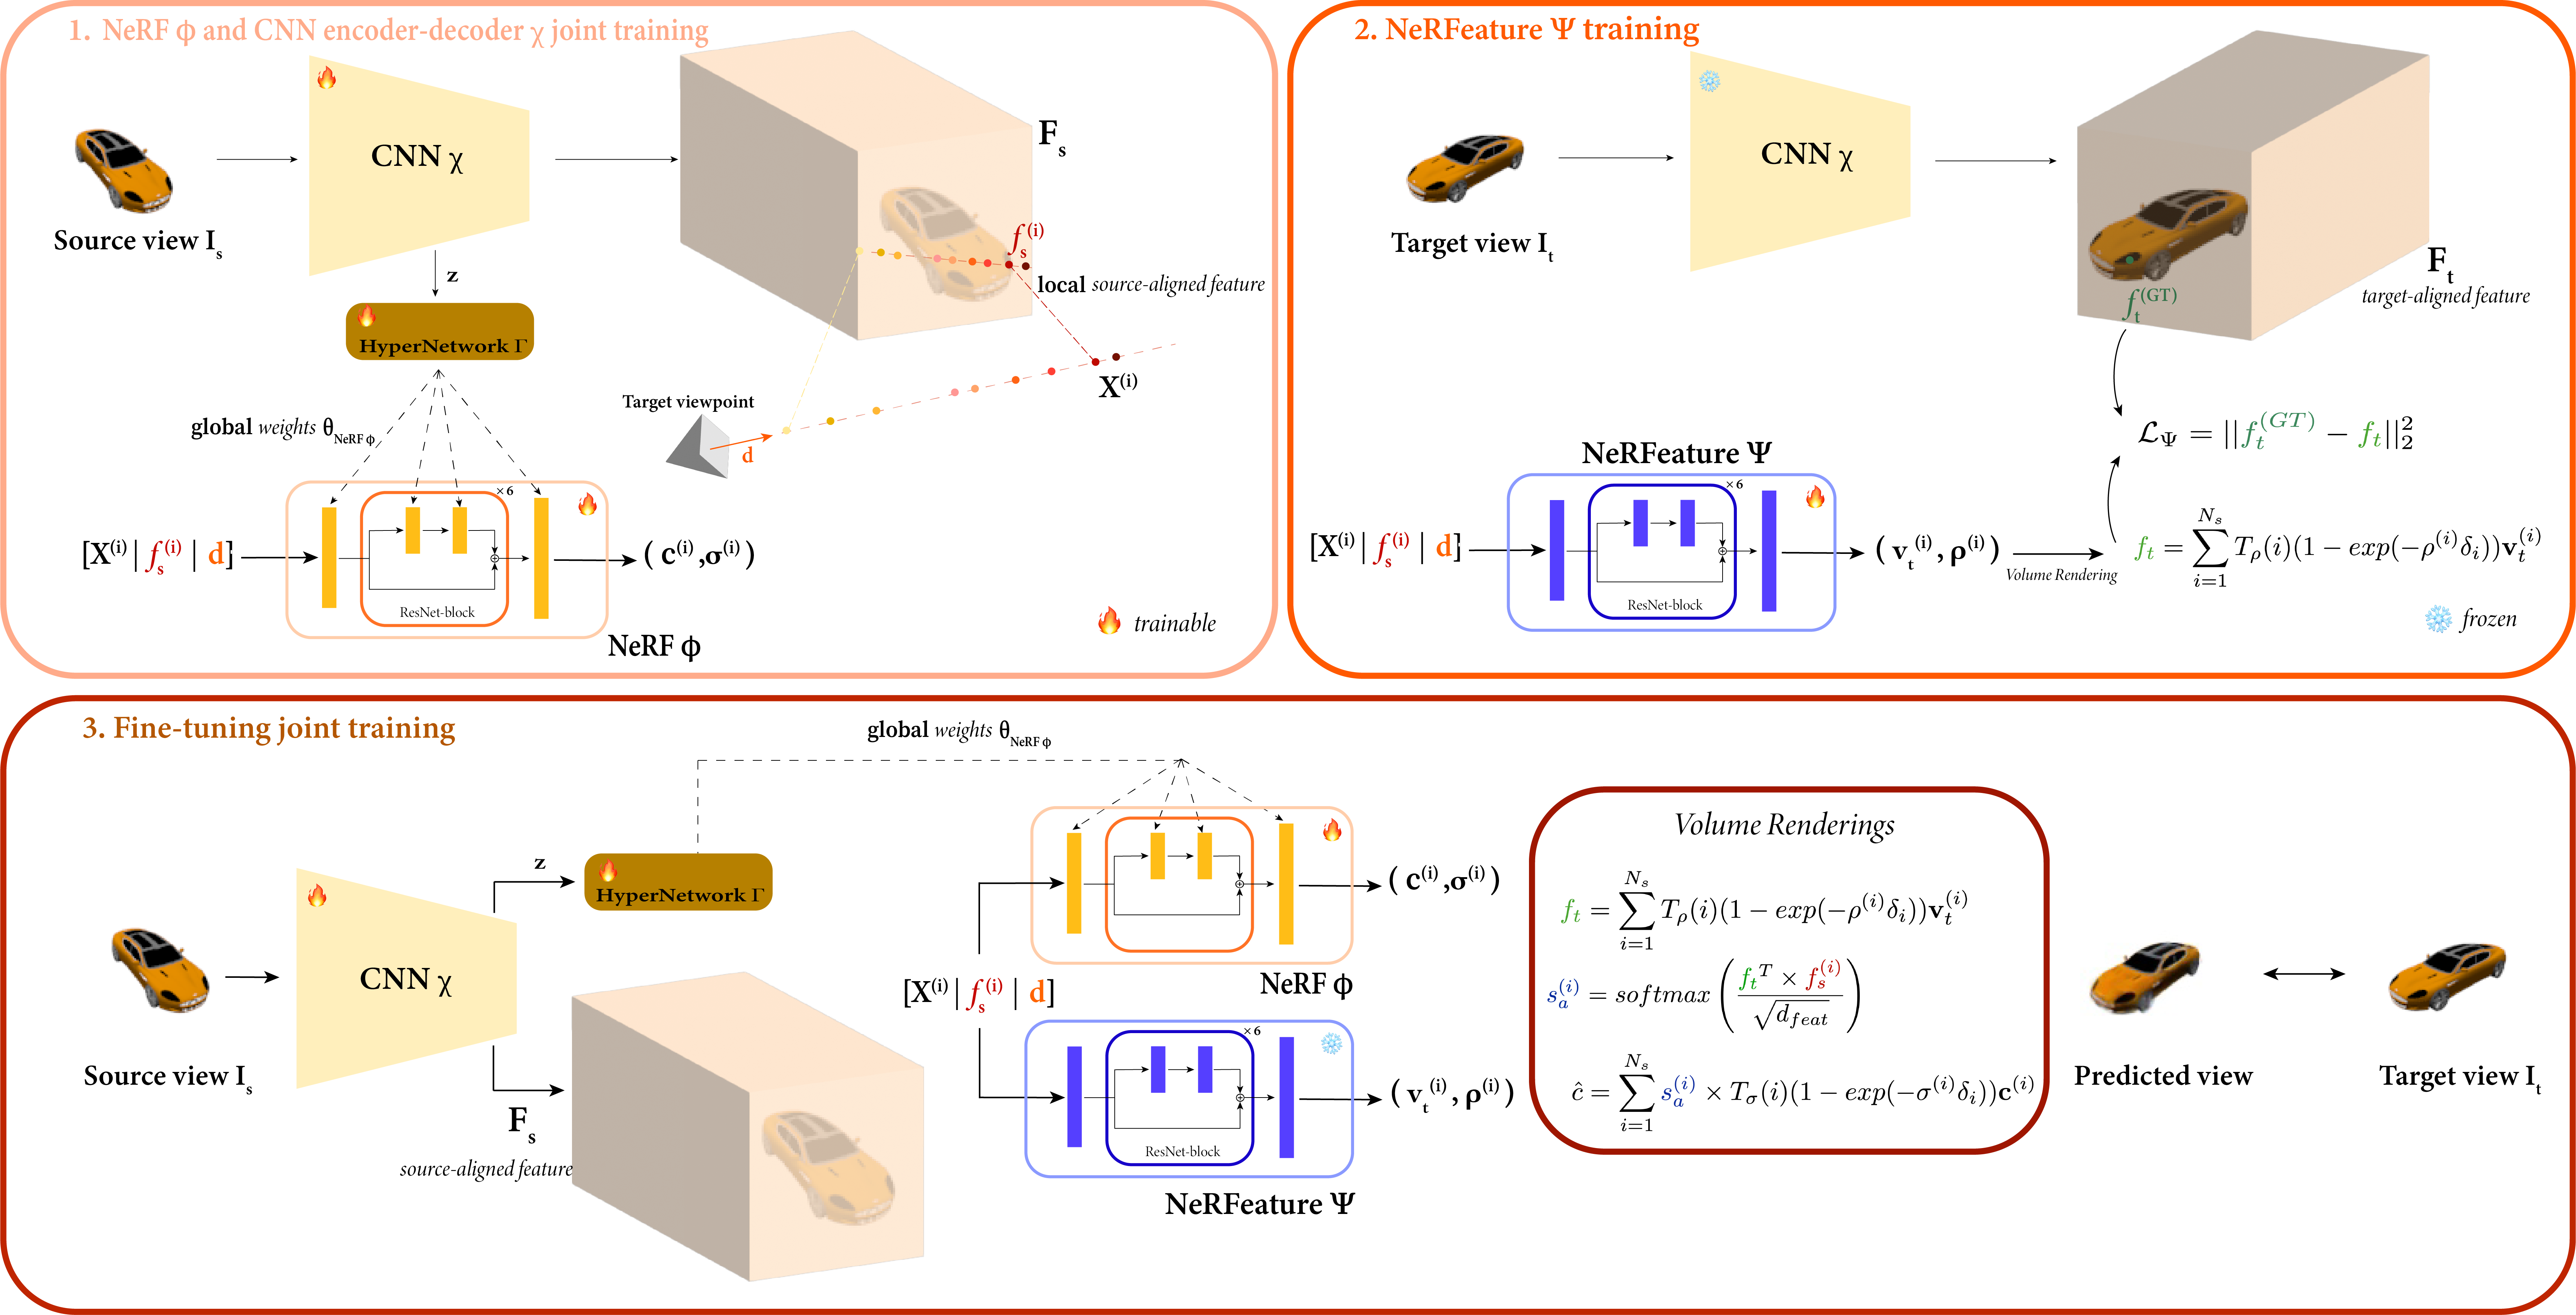
\includegraphics[height=8cm]{images/epinerf/overview_architecture.png}
  \caption{\textbf{Overview of our complete two-stage training EpiNeRF architecture.} (Top left) The first step primarily aims to train our CNN encoder-decoder $\chi$, which can subsequently generates \textit{local} deep features aligned with $I_{s}$. (Top right) Our CNN $\chi$ is then used a teacher model to instruct a residual NeRF student model $\Psi$, termed NeRFeature, to generate such features from any target viewpoint. (Bottom) The second stage training of EpiNeRF is more likely a fine-tuning of both $\chi$ and $\Phi$, with a modified attention epipolar-based volume rendering equation, thanks to the target-aligned feature produced by NeRFeature $\Psi$.}
  \label{fig:overview}
\end{figure*}
\subsection{NeRFeature: learn target-aligned features}
\label{subsec:nerfeature}

While feature volumes produced by any 2D models (CNN or ViT) are defacto aligned with the RGB image they have been fed with (i.e the source image $I_s$), we propose to distil and learn such feature space into 3D through a neural feature radiance field, termed NeRFeature $\Psi$. 

A pretrained teacher 2D CNN encoder $\chi$ (top-left panel on Figure \ref{fig:overview} and subsection \ref{subsec:epinerf}) produces \textit{pseudo} ground truth features, that are used to supervise the training distillation of the NeRFeature $\Psi$ (top-right panel on Figure \ref{fig:overview}).

Given a 3D point $\mathbf{x}^{(i)}$ expressed in the world coordinate system along a ray $\mathbf{r}$ from a target direction $\mathbf{d}$, we denote: 

\begin{equation}
    f_{s}^{(i)} = \mathbf{F}_{s}(\pi(\mathbf{x}^{(i)}))  \in \mathbb{R}^{d_{\text{feat}}} 
    \label{eq:projection}
\end{equation}

the source-aligned feature that was extracted from $\mathbf{F}_{s}=\chi(I_{s})$through the perspective projection $\pi$ of $\mathbf{x}^{(i)}$ on the feature plane.

As the feature radiance field learned through $\Psi$ must be generalizable (\textit{i.e} render meaningful features for unseen objects or scene), NeRFeature has to be input-conditioned on $f_{s}^{(i)}$: 

\begin{equation}
    \Psi(\mathbf{x}^{(i)},\mathbf{d},f_{s}^{(i)}) = (\rho^{(i)},\mathbf{v}_{t}^{(i)}) \in \mathbb{R}_{+}\times \mathbb{R}^{d_{\text{feat}}}
\end{equation}

while the target-aligned feature $\mathbf{f}_{t}$ is obtained through the vanilla volume rendering equation computed over the $N_s$ sampled points on \textbf{r}: 

\begin{equation}
    f_{t} = \sum_{i=1}^{N_{s}} T_{\rho}(i)(1-exp(-\rho^{(i)}\delta_{i}))\mathbf{v}_{t}^{(i)}
\end{equation}

with $\delta_{i}=\mathbf{x}^{(i+1)}-\mathbf{x}^{(i)}$  the distance between two consecutive samples and $T_{\rho}(i) = \exp\left(-\sum_{j=1}^{i}\rho^{(j)}\delta_{j}\right)$ the accumulated transmittance along \textbf{r}.

 Such a learned feature field is finally queried (see Section \ref{subsec:epipolar_att}) during the joint fine-tuning (Figure \ref{fig:overview} - bottom) phase to render target-aligned features, that are involved in an epipolar-based attention mechanism. 
 
\subsection{Feature-based epipolar attention}
\label{subsec:epipolar_att}

As soon as deep feature from $\chi$ has been distilled into the NeRFeature $\Psi$, target-aligned features can be synthesized by solely requiring the source-aligned feature and the corresponding camera relative transformation. A cross-attention distribution \citep{vaswani2017attention} can therefore be computed with such source-aligned features, that all lie on the epipolar line defined by the sampled pixel on the target view. In this way, for any 3D point $\mathbf{x}^{(i)}$, a cross-attention score is obtained from: 

\begin{equation}
    s_{a}^{(i)} = softmax\left(\frac{f_{t}^{T}\times f_{s}^{(i)}}{\sqrt{d_{\text{feat}}}}\right) \in [0,1].
\label{eq:attention}
\end{equation}

The entire distribution $\textbf{s}_{a} \in \mathbb{R}^{N_{s}}$ is obtained by gathering the cross-attention scores for all the $N_s$ projected samples (that all lie on the epipolar line in the source view domain). 

Such an attention score gives an idea of how closed source-aligned features are from the target feature, predicted by $\Psi$. Since it exists an epipolar-based relationship between the location $f_{s}^{(i)}$ and $f_{t}$, the score distribution $\mathbf{s}_{a}$ should has a maximum at the location where target and source pixels exhibit the same content. Associated observation is illustrated on Figure \ref{fig:attention-illustration}. The cross-attention $\mathbf{s}_{a}$ is not used to weight the $\mathbf{f}_{s}$ distribution in the RGB-volume rendering \citep{max1995optical} but rather to adjust the weights distribution $\omega$ that is going to be involved through the inverse transform sampling strategy \citep{mildenhall2020nerf} in the fine NeRF network: 

\begin{equation}
    \omega_{i} = s_{a}^{(i)} \left(1 - \exp(-\delta_{i}\sigma^{(i)})\right)T_{\sigma}(i).
\end{equation}


\subsection{EpiNeRF: the complete architecture}
\label{subsec:epinerf}
\noindent\textbf{CNN-based source-aligned features.} Plethora of recent NeRF-based NVS works leverage their radiance field on a source-aligned feature volume $\mathbf{F}_{s}$, obtained from either a CNN \citep{jang2021codenerf,yu2021pixelnerf,li2022symmnerf} or a ViT \citep{lin2023vision}. However, intermediate features produced by the inner encoder, termed $(\mathbf{F}_{1},\mathbf{F}_{2},\mathbf{F}_{3},\mathbf{F}_{4})$ here,  are often fused and upscaled in a vanilla way, through bilinear upsampling and concatenation in the CNN decoder. The final low-resolution feature volume $\mathbf{F}_{s}$ is obtained through: 
\begin{equation}
    \mathbf{F}_{s} = \left[\mathbf{F}_{1}^{up} || \mathbf{F}_{2}^{up} || \mathbf{F}_{3}^{up} || \mathbf{F}_{4}^{up}\right] \in \mathbb{R}^{2d_{\text{feat}} \times \frac{H}{2} \times \frac{W}{2}}
\end{equation}
where the $[.||.]$ denotes the vanilla concatenation. 

Such a source-aligned feature volume can be built differently, by accounting on residual connections and atrous convolutions, as \citep{chan2023genvs} did too. 
EpiNeRF thus rather gets consideration for DeepLabV3+ \citep{chen2018encoder} as a backbone decoder for the feature volume $\textbf{F}_{s}\in \mathbb{R}^{d_{\text{feat}} \times H \times W}$.  Both upscaling and merging strategies are presented on the Figure \ref{fig:feature_encoder}. 

\begin{figure*}[htb!]
    \center
  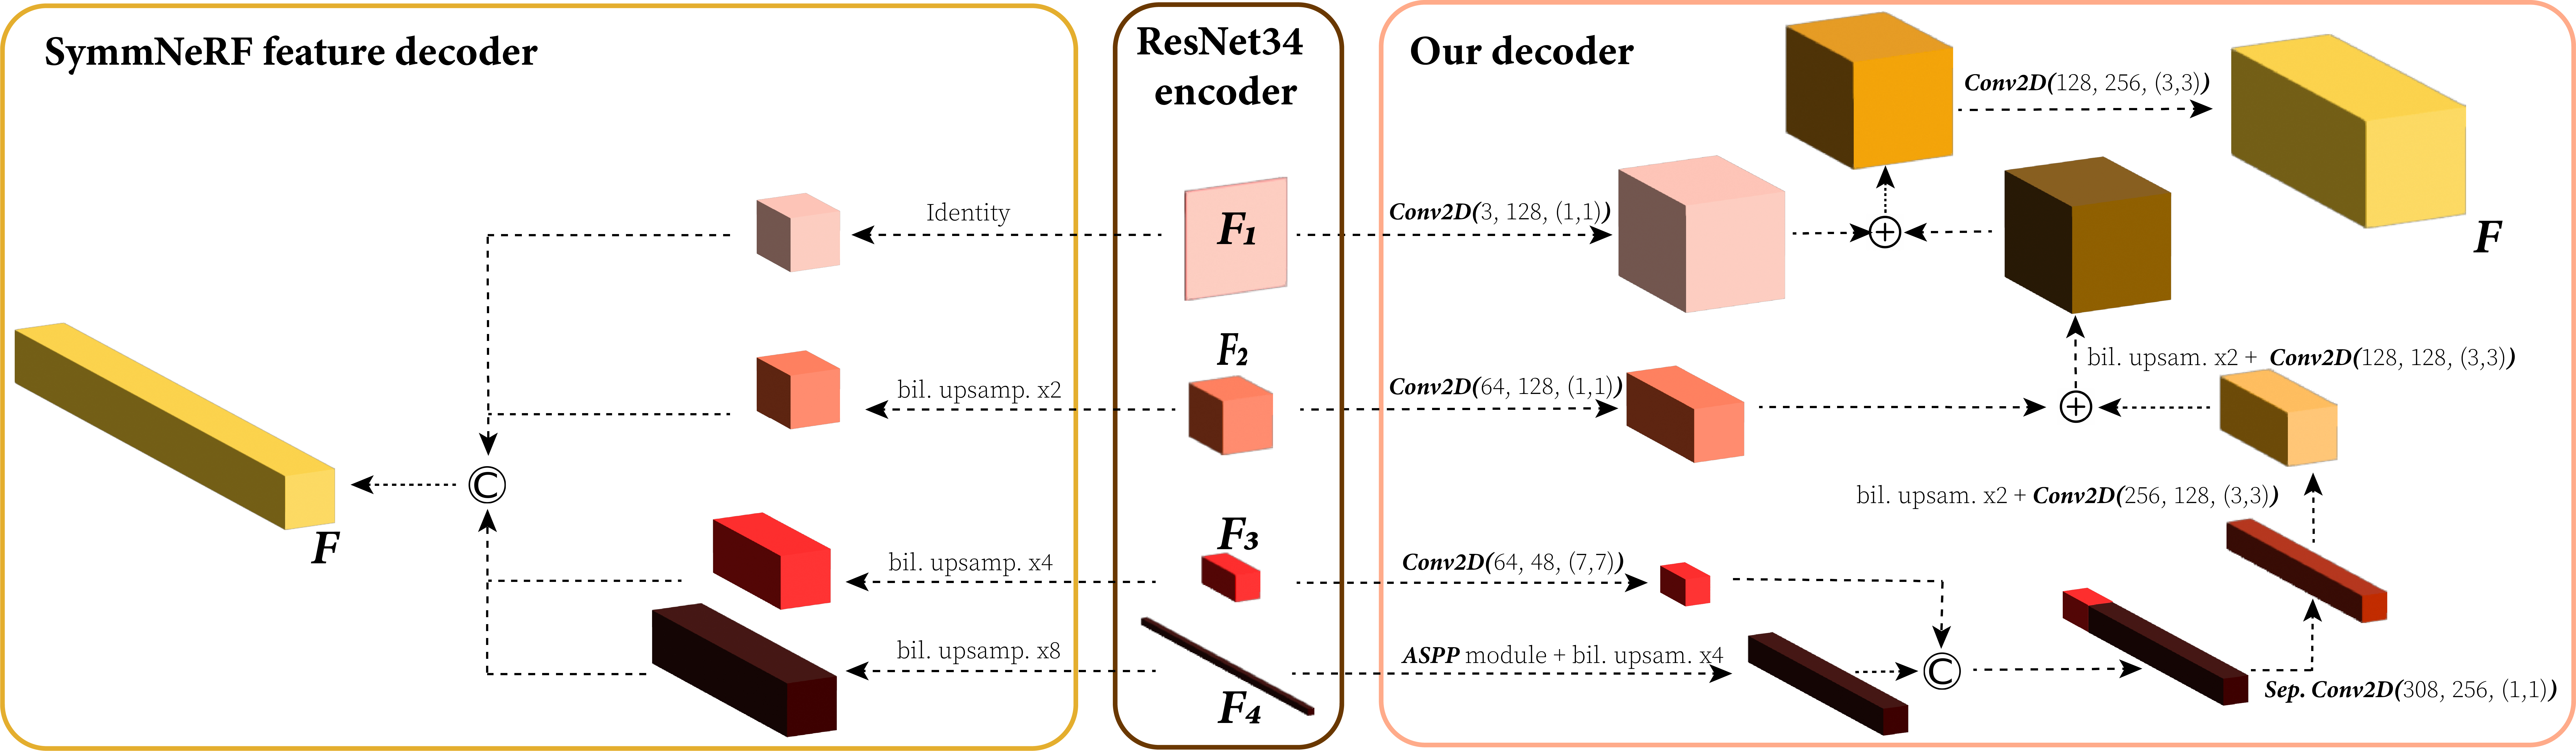
\includegraphics[height=3.5cm]{images/epinerf/feature_fusion_encoder.png}
  \caption{Overview of the CNN decoder $\chi$ involved in SymmNeRF (left) and in our configuration by leveraging on DeepLabV3+ (right). One might note that $\chi$ in both case leverages a ResNet34-based encoder \citep{he2016deep}. }
  \label{fig:feature_encoder}
\end{figure*}
EpiNeRF's feature volume has therefore the same resolution as the input image $\mathbf{I}_s$. While pixel-aligned features are bilinearly interpolated through a 2$\times$2 window, a larger resolution allows better local features sampling that are going to condition the radiance field. \newline

\noindent\textbf{Local and global NeRF conditioning.} Our CNN encoder-decoder $\chi$ primarily produces a set of features $(\mathbf{F}_{1},\mathbf{F}_{2},\mathbf{F}_{3},\mathbf{F}_{4})$ from $\textbf{I}_{s}$. While $\mathbf{F}_{s}$ must be considering as a \textit{local} input conditioning of the radiance fields (since feature are pixel-wise sampled during the perspective projection), we leveraged on an additional MLP network, called a hypernetwork $\Gamma$, that aims to predict NeRF $\Phi$ weights, termed $\theta$, given a latent code $\mathbf{z}$, that is obtained from a non-linear projection of $\mathbf{F}_{4}$. The complete output of our CNN encoder-decoder $\chi$ can thus be re-written as:

\begin{equation}
    \textbf{z}, \textbf{F}_{s} = \chi(I_{s})
\end{equation}
and $\Phi$ is thus  both \textit{locally} (on its input) and  \textit{globally} (through its weights) conditioned: 
\begin{equation}
     \Phi_{\theta}(\mathbf{x}^{(i)},\mathbf{d},f_{s}^{(i)},f_{t}) = (\sigma^{(i)},\mathbf{c}^{(i)}) \hspace{.5cm}\text{;}\hspace{.5cm}  \theta = \Gamma(\mathbf{z})
\end{equation}\newline

\noindent\textbf{Symmetry prior integration.}
Following SymmNeRF \citep{li2022symmnerf} prior work, we made the assumption the (YZ) plane in the canonical coordinates system was a symmetry plane for the implicit 3D scenes we are aiming to reconstruct. It thus involves that a 3D point $\mathbf{x}$ along a target ray \textbf{r} has a symmetrical point with respect to the (YZ)-symmetry plane through:
\begin{equation}
    \mathbf{x}^{(i)}_{symm} = \mathbf{M}\mathbf{x}^{(i)}
\end{equation}
where $\mathbf{M} = \mathbf{I}_{4}\footnote{the Identity matrix in $\mathbb{R}^{4}$} - 2e_{1}e_{1}^{T}$ and $e_{1}$ the first 3D unit basis vector. Such a symmetrical 3D point is back-projected on the source-aligned feature volume $\mathbf{F}_{s}$, as $\mathbf{x}$ was through Equation \eqref{eq:projection}. The \textit{local} deep feature fed to the NeRF $\Phi$ is finally: 
\begin{equation}
    f^{(i)} = \left[f_{s}^{(i)}||f_{s,symm}^{(i)}\right]
\end{equation}

\noindent\textbf{Training.} As depicted on Figure \ref{fig:overview}, our EpiNeRF architecture has a two-step training procedure. It integrates a feature radiance field, termed NeRFeature $\Psi$, in combination with a CNN-based encoder-decoder $\chi$ that \textit{locally} condition the main RGB radiance fields $\Phi$ through an epipolar based attention mechanism. A hypernetwork $\Gamma$ also \textit{globally} conditions $\Phi$, by predicting its learnable parameters through a lightweight MLP network. 

Considering a training set of N objects $\{\mathcal{D}\}_{i=1}^{N}$ with V different viewpoints $\mathcal{D}^{(i)} = \{I_{i}^{(j)},\pi_{i}^{(j)}\}_{j=1}^{V}$ per instance and a batch of rays $\mathcal{R}$, EpiNeRF is optimised through the loss functions: 
\begin{equation}
 \min_{\Psi} \sum_{i}\sum_{j}\mathcal{L}_{\Psi}\left(I_{i}^{(j)},\pi_{i}^{(j)},\Psi,\chi \right) \hspace{.2cm} ; \hspace{.2cm}\mathcal{L}_{\Psi}= \sum_{\mathbf{r}\in\mathcal{R}} || f_{t}(\mathbf{r}) - f_{t}^{(GT)}(\mathbf{r}) ||_{2}^{2}
\end{equation}
and 
\begin{equation}
 \min_{\zeta=\{\chi,\Phi,\Gamma\}}\sum_{i}\sum_{j}\mathcal{L}_{\zeta}\left(I_{i}^{(j)},\pi_{i}^{(j)},\Psi,\zeta \right)\hspace{.2cm}  ; \hspace{.2cm}\mathcal{L}_{\zeta}= \sum_{\mathbf{r}\in\mathcal{R}} || c(\mathbf{r}) - c^{(GT)}(\mathbf{r}) ||_{2}^{2}
\end{equation}


where $c^{(GT)}(\mathbf{r})$ represents the ground truth pixel that was sampled on $\mathbf{I}_{t}$, $f^{(GT)}(\mathbf{r})$ the \textit{pseudo} ground truth deep feature that was sampled $F_{t}=\chi(I_{t})$.
\newline

Deep features produced by NeRFeature are implicitly input-conditioned by $\chi$ since the source aligned feature $f_s^{(i)}$ is fed as input. Hypernetwork $\Gamma$ finally does not have to be trained with a specific loss objective: weights are updated during back-propagation through the vanilla $\mathcal{L}_{2}$ loss function defined over the sampled RGB pixels. 

The second fine tuning training stage is trained in a similar way to the first one, even though NeRFeature weights are now frozen to produce target-aligned features. 

We followed the training strategy that SymmNeRF \citep{li2022symmnerf} and VisionNeRF \citep{lin2023vision} used for $\chi$ and $\Phi$ in both stages and formed batches of 4 images during training, averaged our loss function over 256 rays, and sampled a total of $N_{s}=192$ points along each ray.

\section{Experiments}
\subsection{View synthesis on synthetic data - SRN ShapeNet}
The first presented results were obtained on the ShapeNet dataset \citep{chang2015shapenet}, by focusing on the ShapeNet-SRN \citep{sitzmann2019scene} version. The \textit{Cars} and \textit{Chairs} classes respectively have 3514 and 6591 objects. Training is performed over the 50 different views per instance, while the testing set has 251 views per object, sampled on an Archimedean spiral. We adopted the same evaluation strategy all related works used and considered the view $64^{th}$ as the source image $\textbf{I}_{s}$. Results have been  averaged over the remaining 250 target views. 

Our method reaches state-of-the-art performances according to Table \ref{table:comp_res} and even outperforms the heavier transformer-based architecture \citep{lin2023vision} on almost all metrics. 

\begin{table}[htp!]
\caption{Comparisons against state of the art methods on the category specific \textit{Chairs} and \textit{Cars} classes from the ShapeNet-SRN dataset. Best results are highlighted in red, second ones in orange and third ones in yellow. }
\label{table:comp_res}
\centering%\begin{center}
\begin{adjustbox}{height=2.3cm}
\begin{tabular}[h]{c||ccccccc}
\hline
 Method & \multicolumn{3}{c}{Car} & \multicolumn{3}{c}{Chair} \\
 &  SSIM ($\uparrow$) & PSNR ($\uparrow$) & LPIPS ($\downarrow$) & SSIM ($\uparrow$) & PSNR ($\uparrow$)) & LPIPS ($\downarrow$)\\
\hline
SRN \citep{sitzmann2019scene}& \cellcolor{yellow!25}0.89 & 22.25 & 0.129 & 0.89 & 22.89 & 0.104\\
PixelNeRF \citep{yu2021pixelnerf} & \cellcolor{orange!25}0.90 & 23.17 & 0.146 & \cellcolor{yellow!25}0.91 & 23.72 & 0.128\\
FE-NVS \citep{guo2022fast} & \cellcolor{red!25}0.91 & 22.83 & \cellcolor{yellow!25}0.099 & \cellcolor{orange!25}0.92 & 23.21 & 0.077 \\
GeNVS\citep{chan2023genvs}& \cellcolor{yellow!25}0.89 & 20.7 & 0.104 & - & - & - \\
ShaRF \citep{rematas2021sharf} & \cellcolor{orange!25}0.90 & 22.90 & - & \cellcolor{orange!25}0.92 & 23.37 & - \\
CodeNeRF \citep{jang2021codenerf} & \cellcolor{red!25}0.91 & \cellcolor{orange!25}23.80 & - & 0.90 & 23.66 & -  \\
SymmNeRF\footnotemark\citep{li2022symmnerf}& \cellcolor{orange!25}0.90 & \cellcolor{yellow!25}23.10 & 0.110 & \cellcolor{yellow!25}0.91 & \cellcolor{yellow!25}24.14  & \cellcolor{orange!25}0.075 \\
VisionNeRF \citep{lin2023vision} & \cellcolor{red!25}0.91 & 22.88 & \cellcolor{orange!25}0.084 & \cellcolor{red!25}0.93 & \cellcolor{red!25}24.48  & \cellcolor{yellow!25}0.077 \\
Ours &\cellcolor{red!25} 0.91 & \cellcolor{red!25}24.01 &\cellcolor{red!25} 0.082 &  \cellcolor{orange!25} 0.92 & \cellcolor{orange!25}24.30 & \cellcolor{red!25}0.072 \\

\hline 
\end{tabular}
\end{adjustbox}
%\end{center}
\end{table}
\footnotetext[3]{SymmNeRF\citep{li2022symmnerf} results differ from the ones originally reported by authors since we had to retrain their architecture.}

As depicted in Figure \ref{fig:exp-srn-car}, EpiNeRF successfully gathers best aspects of both SymmNeRF \citep{li2022symmnerf} and VisionNeRF \citep{lin2023vision}. It renders novel views that are simultaneously sharp (eased by the ViT in VisionNeRF) and consistent from a symmetrical perspective on colour patterns (eased by the symmetry prior from SymmNeRF). In this regard, the red left rear door, that is not observed in the source view of the first row,  the right front light on the second one or the white trim in the last example are accurately synthesized by our architecture, contrary to concurrent works that either fail to synthesise sharp views (SymmNeRF) or grasp inherent symmetrical patterns (VisionNeRF). Having a higher-resolution feature volume \textbf{F} helps the radiance field generate sharper results, as shown in section \ref{subsec:visual_insights}. 

\begin{figure}[htb!]
    \center
  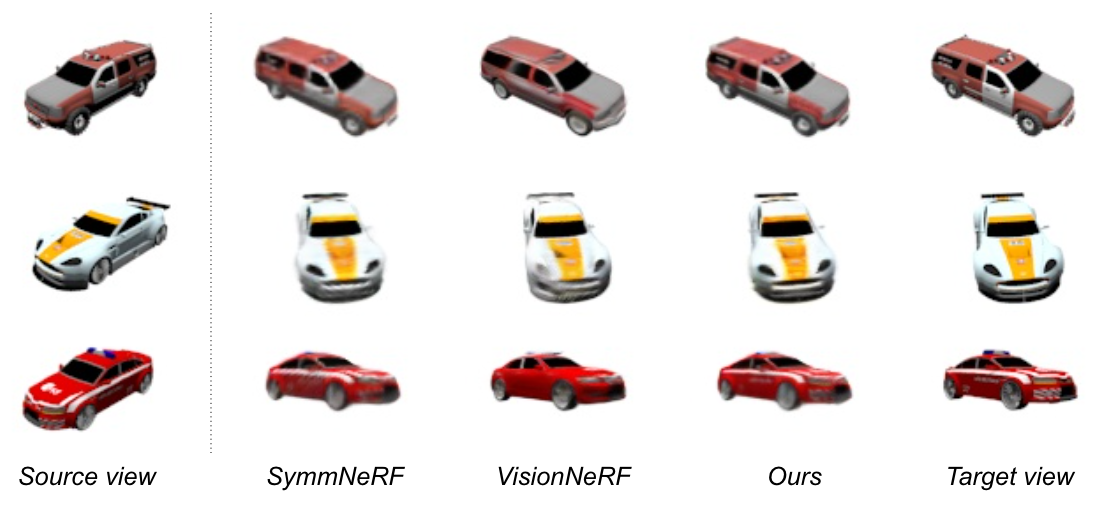
\includegraphics[height=5cm]{images/epinerf/exp-srn-cars.png}
  \caption{Novel view synthesis on the category-specific \textit{Cars} class from ShapeNet. Our method allows to render sharper novel views than SymmNeRF \citep{li2022symmnerf} while maintaining the symmetry that VisionNeRF \citep{lin2023vision} fails to preserve.}
  \label{fig:exp-srn-car}
\end{figure}

 Similar observations can be drawn from the \textit{Chairs} class in Figure \ref{fig:exp-srn-chair}. Intricate geometry on the back and armrests is not entirely synthesised by VisionNeRF  which fails to apprehend how symmetric a chair can be: the armrest structure on the first row is partially missing in the rendered view, even though all the visual information was provided in the source view to render it. SymmNeRF suffers from the same blurry rendering issue that was pointed out in the \textit{Cars} class. Our method offers the best compromise regarding detail retrieval and symmetry reasoning compared to state-of-the-art methods.
 
\begin{figure}[htb!]
    \center
  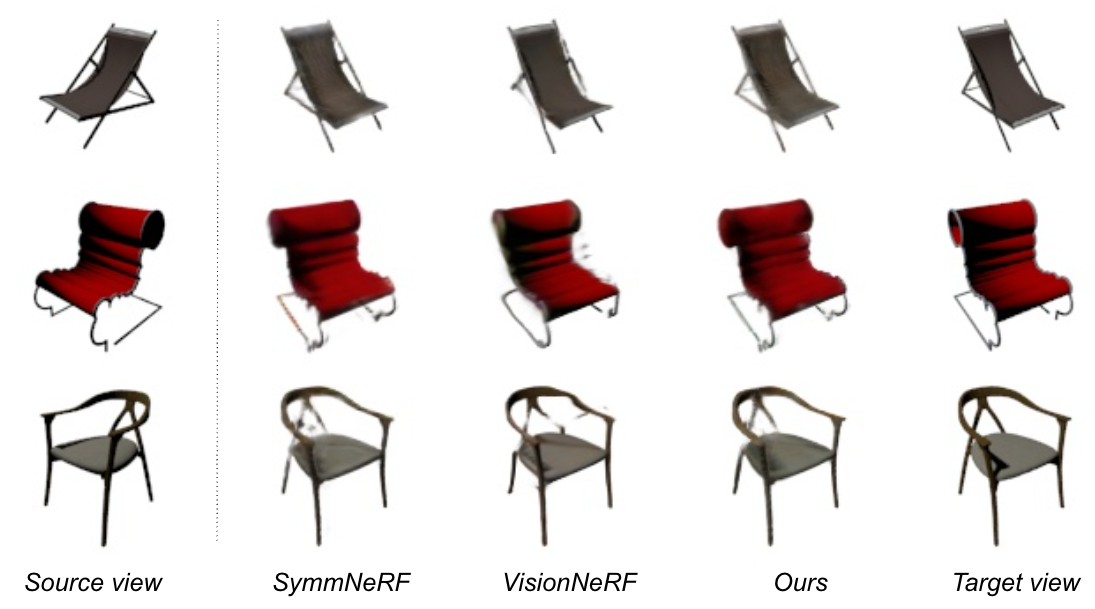
\includegraphics[height=6.1cm]{images/epinerf/exp-srn-chairs.png}
  \caption{Novel view synthesis on the category-specific \textit{Chairs} class from ShapeNet. Tiny structures are not entirely rendered by \citep{li2022symmnerf,lin2023vision} whereas our method manages to reproduce complex back or armrest structures.}
  \label{fig:exp-srn-chair}
\end{figure}

\subsection{View synthesis on real data}
We evaluate our EpiNeRF architecture on real world images, by focusing on the Stanford Cars dataset \citep{krause20133d}. While raw images have been segmented using state-of-the art segmentation model SAM \citep{kirillov2023segment}, images have also been scaled and centred accordingly to match as closed as possible the ShapeNet-SRN image structure. If such a testing scenario is far from the one our architecture has been trained for, Figure \ref{fig:res_Stanfordcar} shows how EpiNeRF is able to produce sharper results than SymmNeRF \citep{li2022symmnerf}, even without any reliable camera pose information.

\begin{figure}[htb!]
    \center
  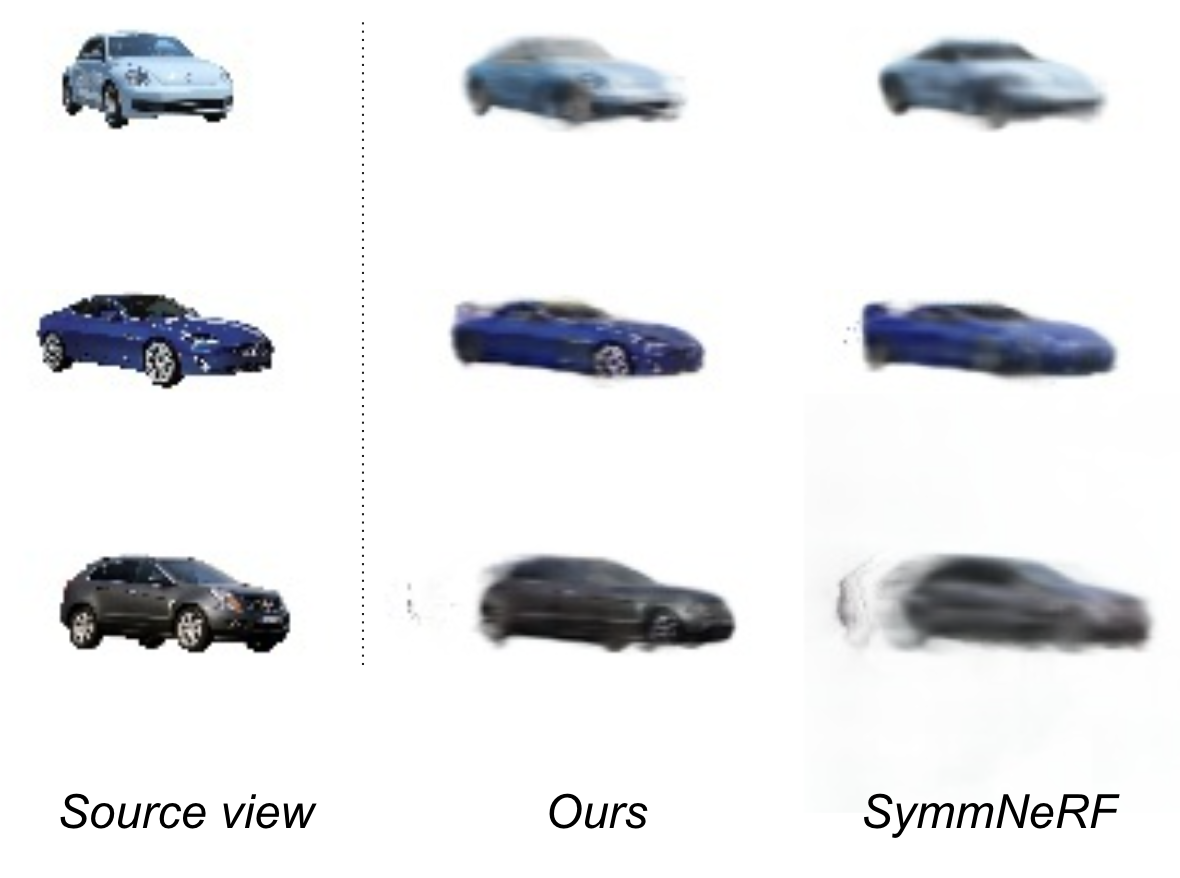
\includegraphics[height=6.cm]{images/epinerf/res_standford_cars.png}
  \caption{Novel view synthesis on the few real \textit{Cars} from the Stanford dataset \citep{krause20133d}. Whereas even closed target viewpoint from the source view leads to fuzzy results, our method render sharper results than SymmNeRF \citep{li2022symmnerf}. }
  \label{fig:res_Stanfordcar}
\end{figure}



\subsection{Ablation study}
Starting with a \textit{baseline} architecture that integrates no symmetry prior information, a vanilla bilinear upsampling strategy to produce $\mathbf{F}_{s}$ and no epipolar attention, we conducted an ablation study to show in which extent each EpiNeRF's components behave on our final novel view rendering architecture. 

\begin{table}[htp!]
\caption{Influence of the different modules onto the final EpiNeRF architecture.}
\label{tab:ablation}
%\begin{center}
\centering
\begin{adjustbox}{width=\textwidth}
\begin{tabular}[h]{c||ccccccc}
\hline
Method & \multicolumn{3}{c}{Car} & \multicolumn{3}{c}{Chair} \\
 &  SSIM ($\uparrow$) & PSNR ($\uparrow$) & LPIPS ($\downarrow$) & SSIM ($\uparrow$) & PSNR ($\uparrow$)) & LPIPS ($\downarrow$)\\[.5pt]
\hline
baseline & 0.89 & 22.71 & 0.108 & 0.90 & 23.03 & 0.090 \\[1.5pt]
\hline 
+ Symmetry constraint \citep{li2022symmnerf}  & \ 0.90 & 23.10  & 0.110 & 0.91 & 24.14 & 0.075 \\
+ DeepLabV3 CNN encoder  & \cellcolor{red!25}{0.91} & 23.87 & 0.087 & \cellcolor{red!25}{0.92} & 24.23 & 0.073 \\
+ Epipolar Attention  & \cellcolor{red!25}0.91 & \cellcolor{red!25}24.01 &\cellcolor{red!25}0.082 & \cellcolor{red!25}0.92 &  \cellcolor{red!25}24.30 &\cellcolor{red!25}0.072 \\
\end{tabular}
\end{adjustbox}
%\end{center}

\end{table}

As shown on Table \ref{tab:ablation} and visually confirmed on Figure \ref{fig:ablation}, integrating the symmetry prior helps the network to better grasp symmetrical and complex pattern structures, whereas the high-resolution feature volume produced by our encoder-decoder $\chi$ leads to sharper edges and thinner structures in RGB space. Finally, the feature attention-based epipolar module, that involved both source-aligned (from $\chi$) and target-aligned (from NeRFeature $\Psi$) features improves the overall quality of the EpiNeRF rendering. 

\begin{figure}[htp!]
    \center
  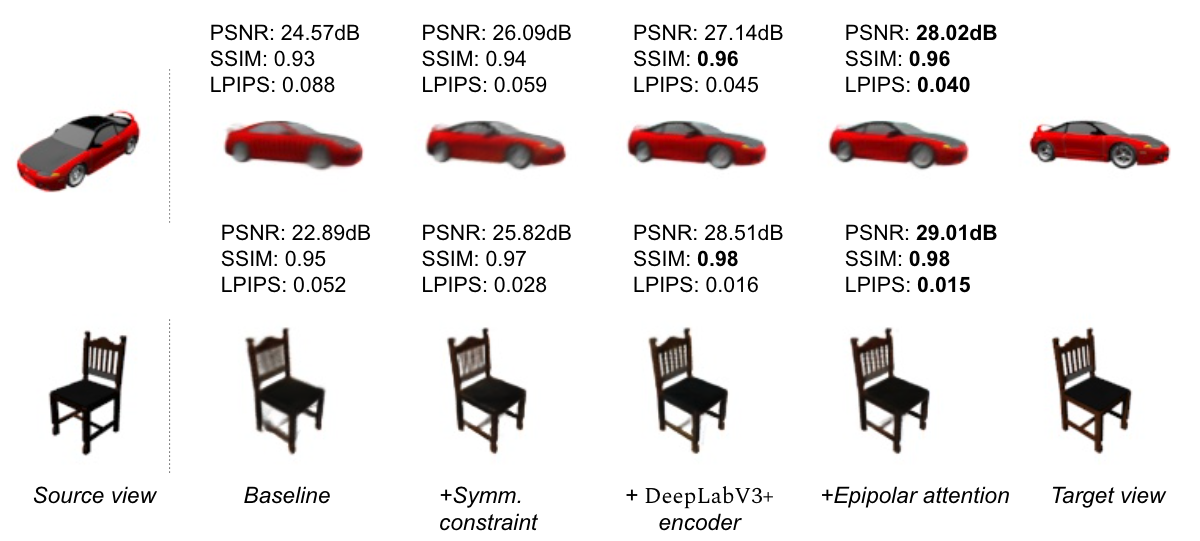
\includegraphics[height=5cm]{images/epinerf/ablation-srn.png}
  \caption{Visual influence of the different modules and constraints that were progressively applied to our architecture on ShapeNet-SRN dataset.}
  \label{fig:ablation}
\end{figure}


\subsection{Feature and attention visual insights}
\label{subsec:visual_insights}


\paragraph{Target-aligned feature synthesis with NeRFeature.} 
Whereas primary purpose of NeRFeature is not to generate an entire feature map from a target viewpoint, one can generate such an $\mathbf{F}_{t}$ deep volume given a source image $I_{s}$ and a corresponding relative camera transformation. Results are depicted on Figure \ref{fig:nerfeature_prediction}. 

\begin{figure*}[htb!]
  \centering
  \begin{subfigure}[t]{0.45\linewidth}
    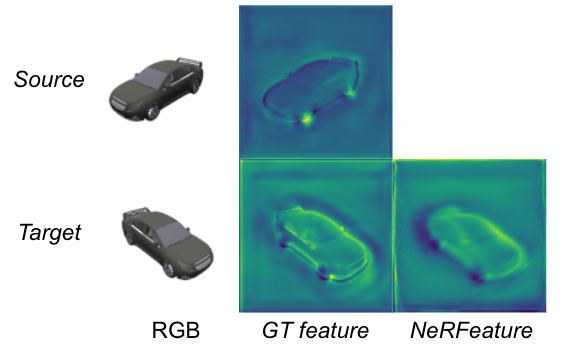
\includegraphics[height=3cm]{images/epinerf/nerfeature.png}
    \caption{\textit{Pseudo} ground truth features are generated through our CNN encoder-decoder $\chi$. Only the first channel are depicted shown for an illustrative purpose.}
    \label{fig:nerfeature_prediction}
  \end{subfigure}
  \hfill
  \begin{subfigure}[t]{0.51\linewidth}
    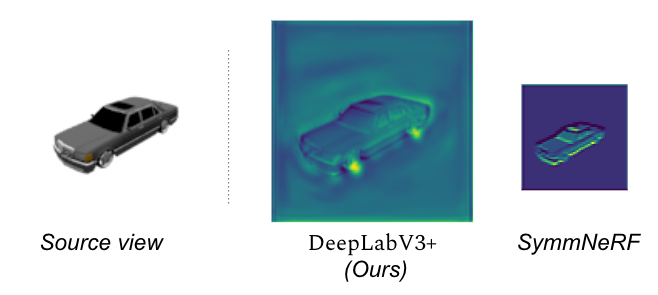
\includegraphics[height=3.cm]{images/epinerf/feature_visuals.png}
    \caption{Feature map \textbf{F} produced by our encoder (\textit{center}, 128$\times$128 spatial res.) and by SymmNeRF (\textit{left}, 64$\times$64 spatial res.) given a source view (\textit{right}, 128$\times$128 spatial res.)}
    \label{fig:featuremap_comparison}
  \end{subfigure}
  \caption{Feature map respectively observed from a target - NeRFeature $\Psi$, \ref{fig:nerfeature_prediction} - and source - CNN $\chi$, \ref{fig:featuremap_comparison} - viewpoint perspective. }
  \label{fig:short}
\end{figure*}

As observed, the overall pose of the target-aligned feature is properly inferred by our feature radiance field $\Psi$, even through tiny details fails to be accurately retrieved (e.g on windows). 

\begin{figure*}[htb!]
  \centering
  \begin{subfigure}[t]{0.48\linewidth}
    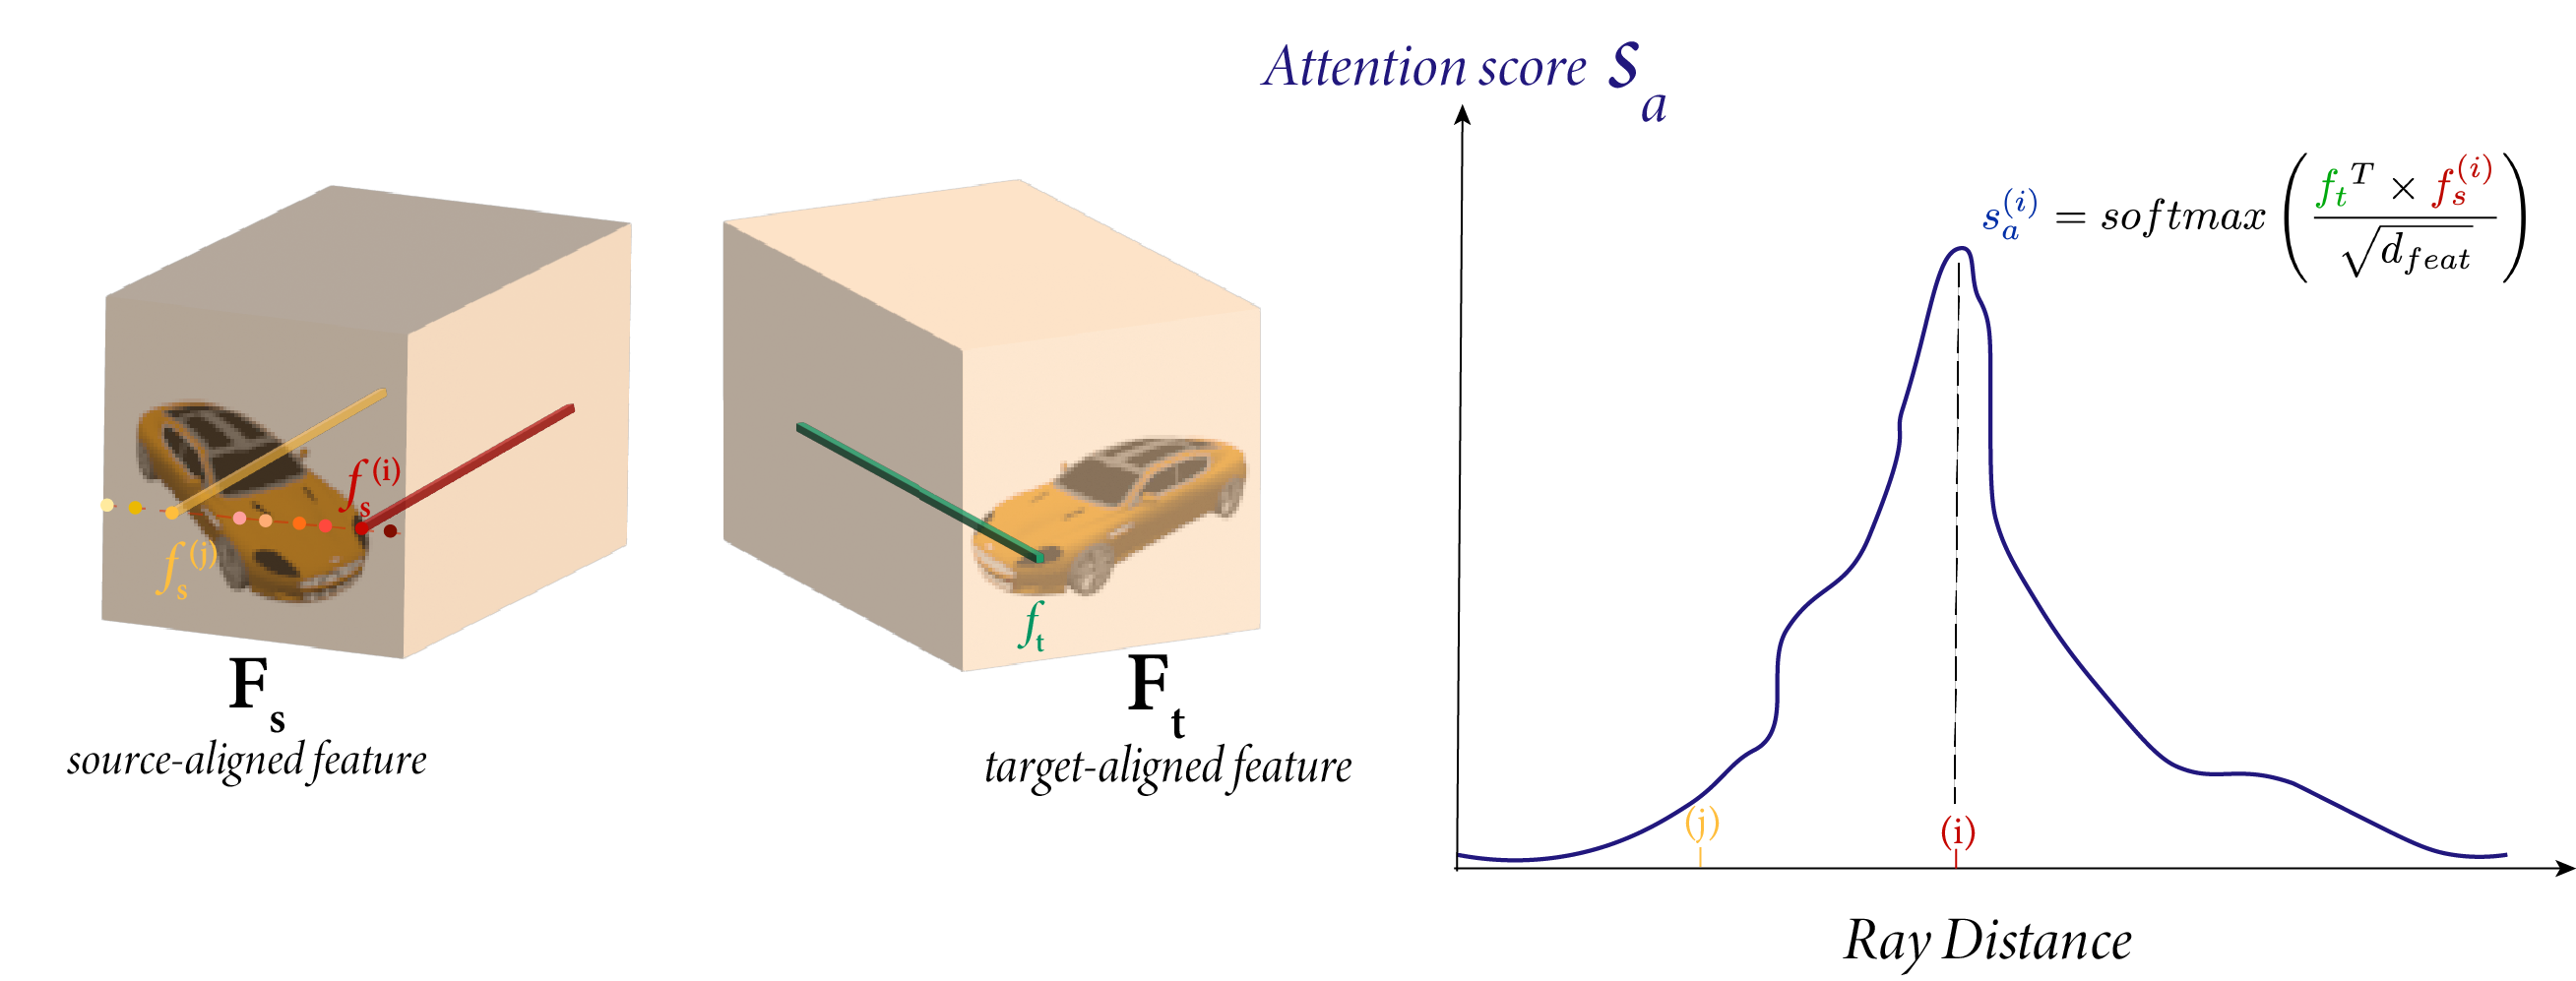
\includegraphics[height=2.4cm]{images/epinerf/attention_illustration.png}
    \caption{Toy feature attention distribution example along a ray. Two closed features that respectively lie in the source and target-aligned feature volume should exhibit a high cross-attention score.}
    \label{fig:attention-illustration}
  \end{subfigure}
  \hfill
  \begin{subfigure}[t]{0.48\linewidth}
    \center
    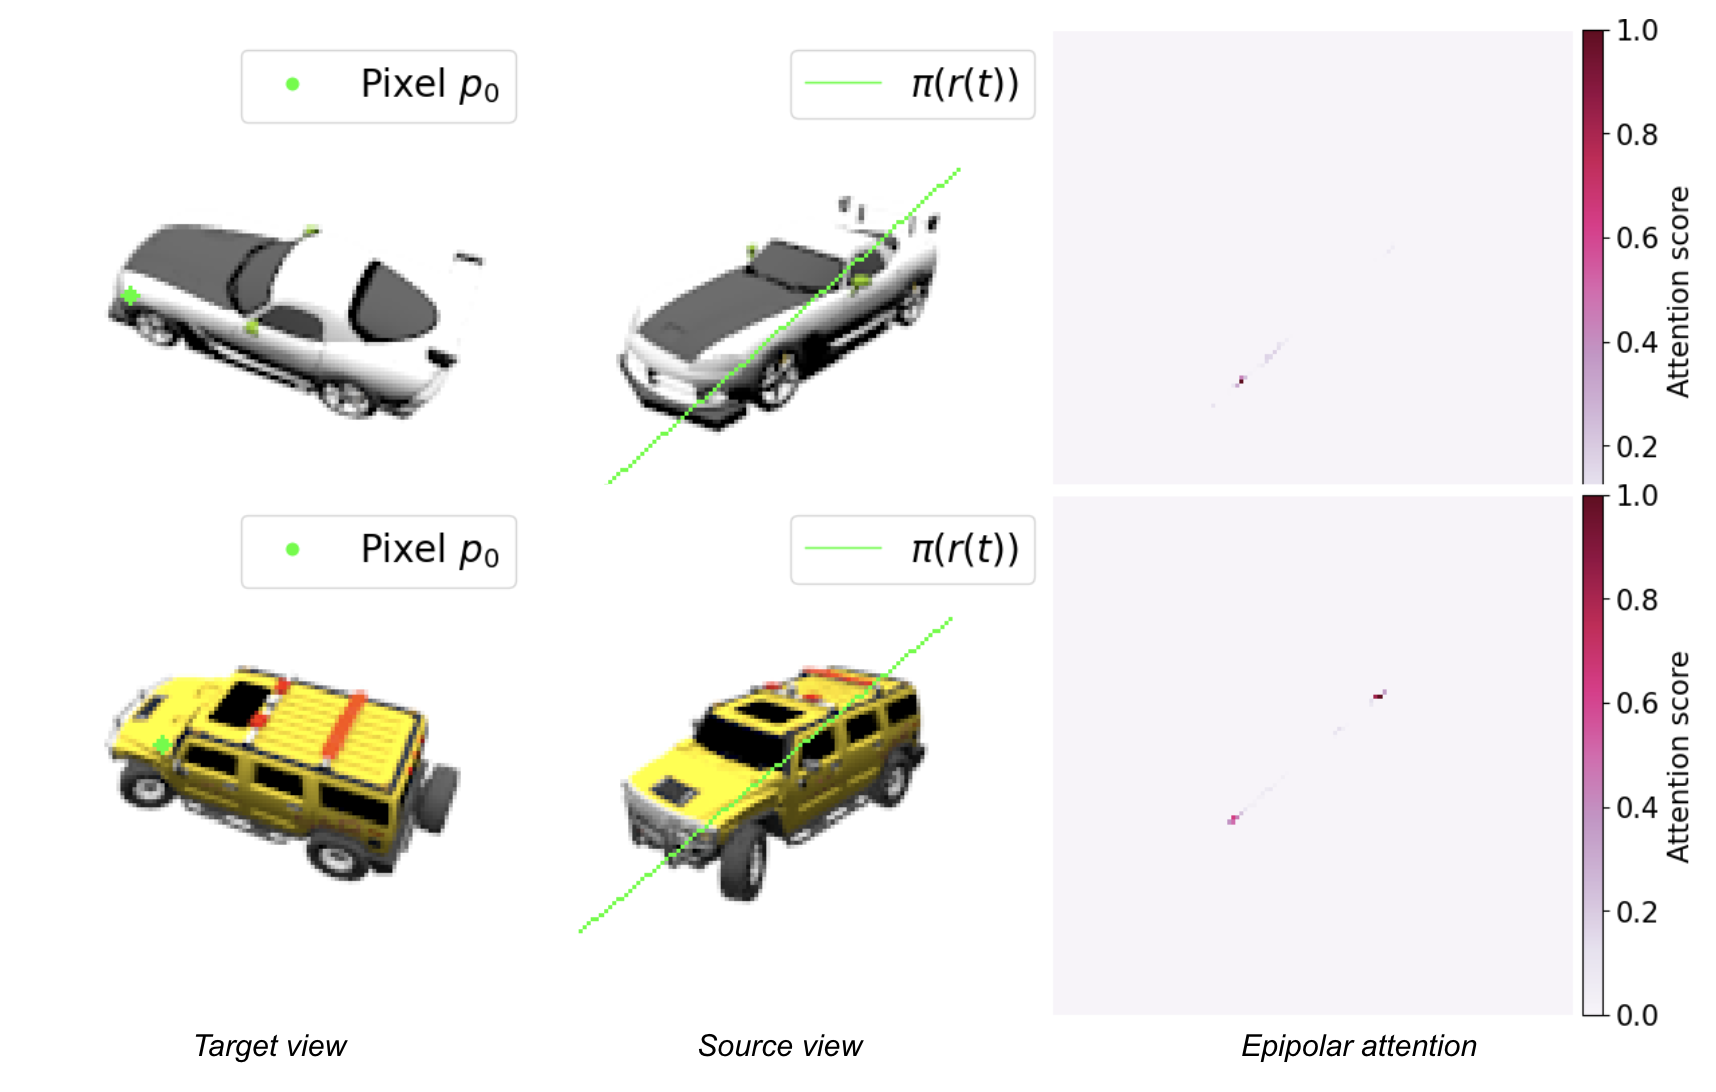
\includegraphics[height=3.3cm]{images/epinerf/exp_epipolar_attention.png}
    \caption{Epipolar attention activation in two different scenarios: While sampling empty area results in low attention scores across the whole epipolar line (top row), proper car areas sampling lead to tightened attention distribution (bottom row).}
    \label{fig:attention-practice}
  \end{subfigure}
  \caption{ \ref{fig:attention-illustration} Source-target feature attention conceptual idea along a ray. \ref{fig:attention-practice} In-practice epipolar-based attention distribution on two instances.}
  \label{fig:attention}
\end{figure*}





\paragraph{CNN encoder-decoder $\chi$.}
Since the EpiNeRF's feature map has the spatial resolution of the source view, first layers of $\textbf{F}_{s}$ should exhibit sharper edges and details compared to SymmNeRF. Figure \ref{fig:featuremap_comparison} tends to confirm such claim: complex regions as on the front part of the car are more coarse in SymmNeRF than on our feature map. Our feature maps are, by design, twice as resolved as those of SymmNeRF, achieving a resolution of $128\times128$. 


\paragraph{Epipolar attention.}
We depict in this last subsection some visuals insights regarding our epipolar attention module. As shown on the second row of Figure \ref{fig:attention-practice}, sampling a target pixel on the yellowish front part of the car will, on the corresponding epipolar line, results in the highest activation closed to the same regions, in the source view domain. 

\section{Limitations \& future work}
While our work address several drawback in existing state-of-the-art methods through the design of target-aligned features, room remains for additional investi\--gations in future works. As the NeRFeature $\Psi$ is an complementary network in our EpiNeRF architecture, inference time is slower than the baseline architecture we considered. However, instead of using two NeRFs ($\Phi$ and $\Psi$) in our EpiNeRF model, one can explore the possibility of only using a single radiance field, namely ($\Phi$), with an additional inner branch devoted to the prediction of the target-aligned features. Such improvement should decrease the inference time closed to the baseline we worked on. 


\section{Conclusion}

In this paper, we propose a new NeRF-based single-image NVS architecture. The NeRF architecture relies on an original CNN-based \textit{local} and \textit{global} conditioning; local since the CNN representation of the source image pixels is used as NeRF's input and global as the whole learnable NeRF's weights are obtained via an hypernetwork that leverages last CNN's layer. The proposed method can thus be summarised as follow: 1) A first NeRF is leaned to give access to high resolution source-aligned features ; 2) This set of features is distilled by the training a second radiance field, termed NeRFeature, that aims to predict high resolution target-aligned features. These two NeRFs and the CNN that conditioned them are merged together to form the proposed EpiNeRF architecture; 3) In a final stage, EpiNeRF is fine-tuned. EpiNeRF main innovation lies on the epipolar constraint that is implemented in the RGB volume rendering via a feature-based attention mechanism. The main strength of such a constraint lies on its $d_{\text{feat}}$-dimensional computation, using a softmax score obtained from both source and target-aligned features. Theses contributions enables EpiNeRF to improved 3D points sampling and consequently achieve a more realistic final rendering result compared to current state-of-the-art methods. We demonstrated our claims on synthetic and real-world datasets, pushing towards better integration of 3D priors including epipolar and symmetrical constraints within generalizable NeRF architectures. 
  







\cleardoublepage
\let\leftmark=\oldleftmark

\acresetall
\chapter{Gaussian Splatting for 360\degree spin stabilization}
\label{chapter:gausssplat}

\chapterwithfigures{\nameref*{chapter:gausssplat}} \chapterwithtables{\nameref*{chapter:gausssplat}}

\ifthenelse{\boolean{skipGauss}}{\endinput}{}


% Math symbol

\section{Introduction}
This final section extends the latest two sections that were mostly focused toward a research academic perspective. Core motivation rather lies here on the desire to apply \ac{NVS} latest advances on an industrial project, where processed images resolution are at least $10\times$ higher than ShapeNet-SRN \citep{chang2015shapenet,sitzmann2019scene} ones ($\sim$ 1-2K against $128\times128$). \ac{NeRF} have benefited over the latest few years from massive improvements against several directions; training time, camera pose requirements, inference speed, drastic model weight reduction \textit{etc}. 
However, \ac{NeRF}-based methods suffers from an intrinsic computational bottleneck at inference time. It requires to query the \ac{NeRF} roughly 500 millions times to generate a squared $2K\times2K$ image. As a direct consequence, one of the most acknowledged state-of-the-art method, termed Mip-NeRF360 \citep{barron2022mip}, is only able to render at < 0.1 \ac{FPS} a 1080p image. It would therefore be necessary to deploy a lot of \ac{GPU} resources and engineering refactorization to properly parallelize the source code in order to synthesize novel views at acceptable speed. 

We thus work in this section with a different set of constraints. First concerns the generalizable property we kept in the two previous sections. We do not aim anymore to build or rely on an algorithm that can synthesize a viewpoint from any image belonging to a specific class. We thus rather want to leverage on \textit{per-scene} framework, that would require a novel training as soon as we work with a new scenario. Furthermore and as mentioned earlier, images we are now working with are closer to what clients could sent to any \ac{AI} SaS company, both regarding resolution and content. Finally, camera poses are no longer available as ground truth since real-world images CarCutter by Meero has to deal with are unposed. They thus must be first estimated using \ac{SFM} techniques (subsection \ref{subsec:gs-sfm}).

Core idea is rather to leverage on the very latest advances in neural rendering, mostly on \ac{GS} ones. \ac{GS} offers an extremely well balanced trade-off between rendering quality and training/inference requirements. Contrary to \ac{NeRF}-based methods, that are therefore often too slow to render high-resolution images, \ac{GS} shows an outrageously 100 \ac{FPS} performance, withtout relying on any neural network architecture. However, the \ac{NVS} paradigm we were used to deal with until now has heavely changed: View synthesis is not anymore infered given a source image and a camera transformation. As soon as \ac{GS} reconstructs the whole 3D scene through a set of 3D coloured gaussians, render a novel view now at a specific viewpoint only require a camera pose information.


\section{Background}
In order to be as close as possible to what was investigated for CarCutter and to remain consistent accross the experiments and tested methods, a single scene made of 36 views is used in this section. Figure \ref{fig:gs-original_scene} depicts such scene. This background section establishes fundamental concepts and algorithms that turn such an unordered and unposed finite set of images into an explicit 3D scene that can be rendered from any viewpoint. 

\begin{figure}[htb!]
  \centering
  \begin{subfigure}[b]{0.45\linewidth}
    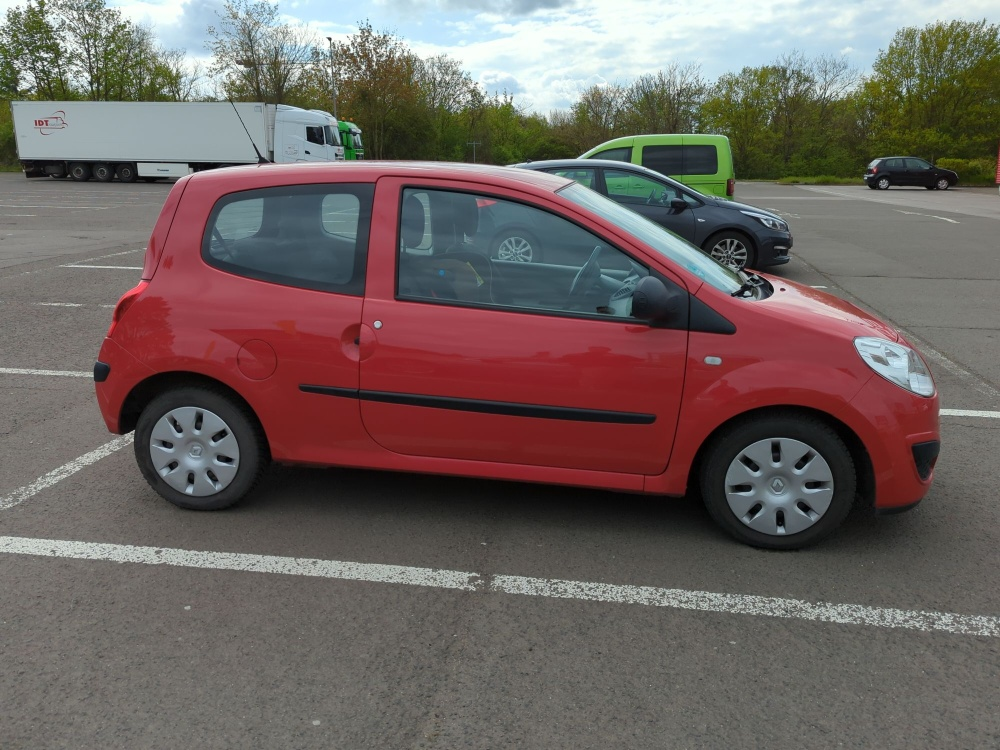
\includegraphics[width=\linewidth]{images/gaussiansplatting/gt/img-4.jpg}
    \caption{\textbf{A random view.} The view indexed \textit{0004} is represented here for an illlustrative purpose. }
    \label{fig:view-idx-4}
  \end{subfigure}
  \quad % Space between the figures
  \begin{subfigure}[b]{0.45\linewidth}
    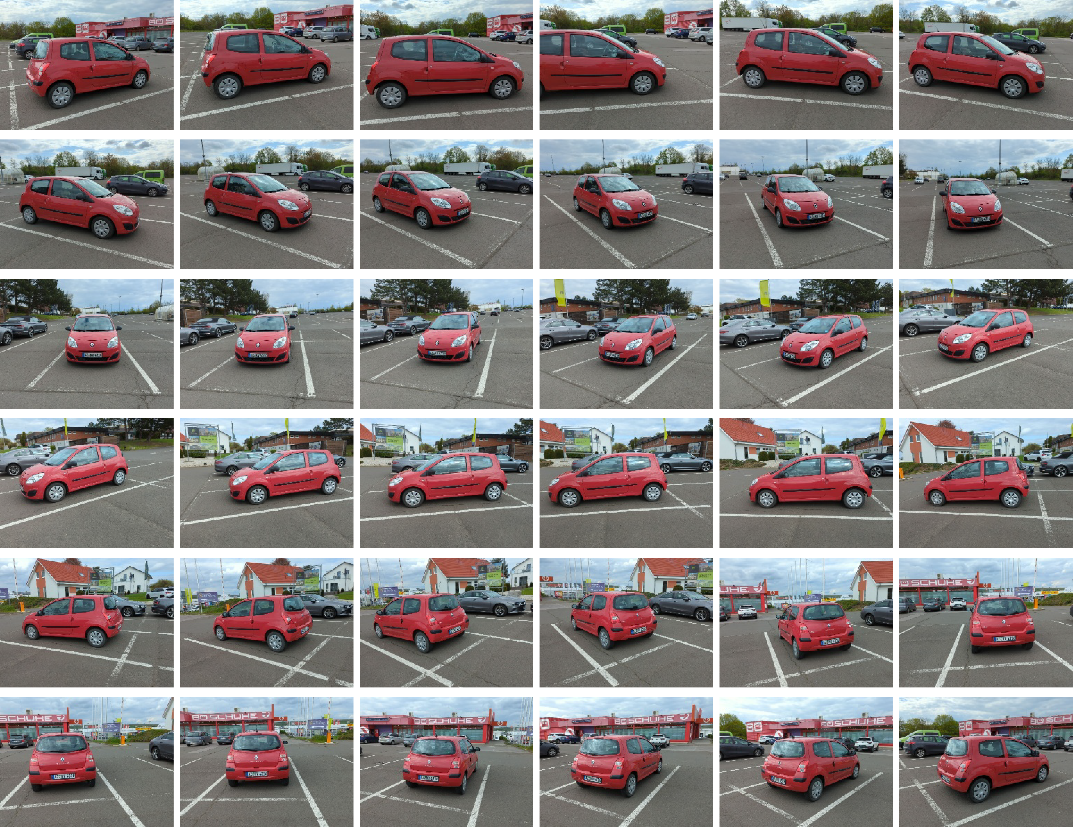
\includegraphics[width=\linewidth]{images/gaussiansplatting/original_scene.png}
    \caption{\textbf{Original scene.} Such a scene is typically what Carcutter is working with on a daily basis. A total of 36 unposed views has been acquired here. }
    \label{fig:gs-original_scene}
  \end{subfigure}
  \caption{\textbf{Scene set overview} The considered scene as 36 $1500\times2000$ photographs that were taken by hand without any tripod nor specific equipment. }
  \label{fig:gs-scene-dataset}
\end{figure}

\subsection{Camera pose estimation through SfM with COLMAP}
\label{subsec:gs-sfm}

\begin{figure*}[htb!]
    \center
  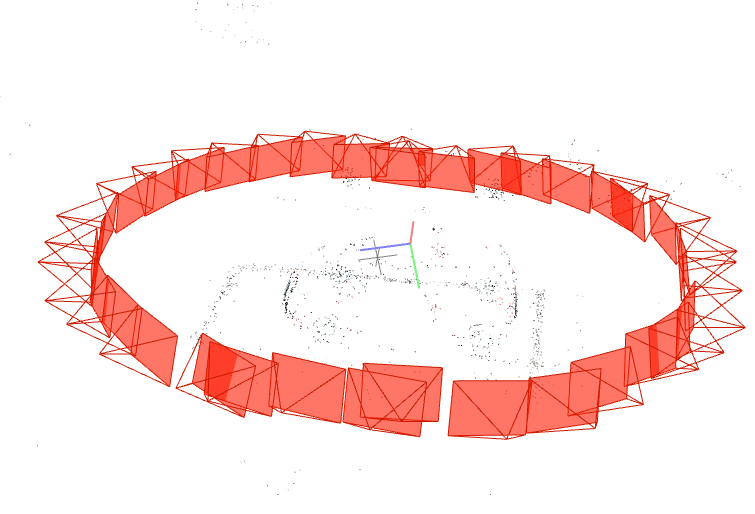
\includegraphics[height=8cm]{images/gaussiansplatting/colmap_sparsePC.png}
  \caption{\textbf{COLMAP 3D sparse reconstruction.} Given the set of unorded and unposed 36 views depicted below, COLMAP reconstructs an extremely sparse coloured point cloud with the corresponding estimated camera location. A total of $N=4105$ points has been registered here in this scenario.}
  \label{fig:gs-sfm}
\end{figure*}


\subsection{Gaussian Splatting}
\label{subsec:gs-gs}

It exists a plaethora of different ways to represent 3D data, either explicitly (such as point clouds, meshes) or implicitly. \ac{NeRF} implicitly embeds the whole structure and texture of a scene in its inner weights: an image is rendered by sampling points on casted rays and quering the architecture accordingly. \ac{GS} rather leverages on a 3D gaussian primitive to explicitly model the 3D scene and get a fully differentiable pipeline that can solely be supervised at 2D-image level. Figure \ref{fig:gs-overview} gives few insights regarding how such a pipeline is built.  

\begin{figure*}[htb!]
    \center
  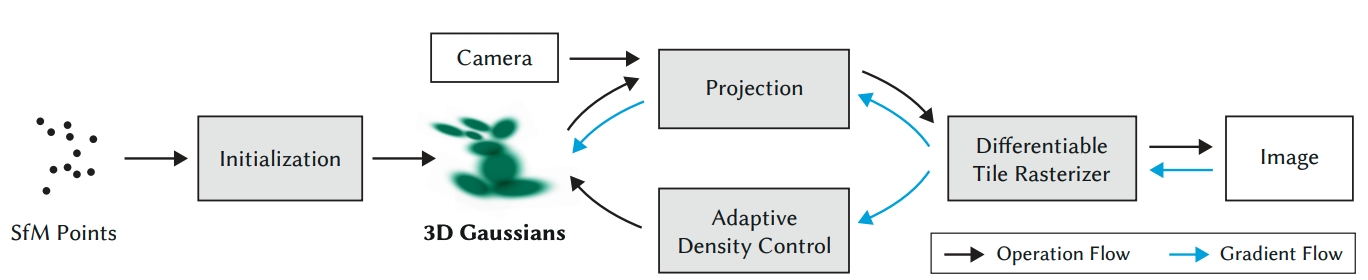
\includegraphics[width=\linewidth]{images/gaussiansplatting/overview-pipelineGS.png}
  \caption{\textbf{Gaussian Splatting pipeline overview.} Starting from a sparse 3D point cloud, \ac{GS} is designed on a lightweight and differentiable pipeline that does not involve any deep or shallow neural architectures.}
  \label{fig:gs-overview}
\end{figure*}

We present below the key steps that were defined in the original \ac{GS} seminal work \citep{kerbl20233d}.

\noindent \textbf{Initialization} From a sparse coloured \ac{SFM}-3D point cloud, refered as $\mathcal{P}\in\mathbb{R}^{N\times(3+3)}$, an associated set of 3D Gaussians $\{\mathcal{G}_{k}|k=1,...,K\}$ is build. Each primitive $\mathcal{G}_{k} $ has therefore an attached set of attributes $\{\mu_{k},\Sigma_{k},c_{k},\alpha_{k}\}$, defined by: 
\begin{itemize}
    \item A mean $\mu_{k}$, corresponding to the original point location in $M$. 
    \item A covariance $\Sigma_{k}$ $3\times3$ matrix, that must be positive semi-definite. Initialized to be isotropic. 
    \item A color $c_{k}$, represented using \ac{SH} coefficients. Additional information regarding \ac{SH} theory and construction can be found in the Appendix \ref{appendix:gs-sh}. 
    \item An opacity/transparency $\alpha_{k}$ value. 
\end{itemize}

While mean, color and opacity can be optimized without any constraints with gradient-descent based algorithm, $\Sigma_{k}$ has to remain semi-definite positive \footnote{\textit{i.e} $ \forall a \in \mathbb{R}^{3}: a^{T}\Sigma_{k} a \geq 0$} during training to represent a meaningful 3D coviance matrix. As holding this constraint during the optimization would be to complex, $\Sigma_{k}$ is factorized (as an eigendecomposition) in the world coordinate system via with a rotation matrix $O_{k}$ (analytically expressed with 4 quaternions) and a scaling vector $s_{k}$: 

\begin{equation}
    \Sigma_{k} = O_{k}s_{k}s_{k}^{T}O_{k}^{T}
\end{equation}
As any matrix expressed with $A^{T}A$ is always semi-definite positive, $\Sigma_{k}$ is now properly constrained. Term $O_{k}s_{k}$ has to be seen as scaled rotation matrix, where $O_{k}$ defines the Gaussian $\mathcal{G}_{k}$ rotation in space and $s_{k}$ its size. 

These attributes that are going to be learned, for all gaussian primitives during training. The table \ref{tab:gauss-param} summarizes the total number of parameter that need be be optimized for each gaussian. 

\begin{table}[h!]
  \centering
  \begin{tabular}{lcc}
  \hline
  Parameter  & Size & Note \\
  \hline
  Position (mean)  $\mu$ & 3 & 3D vector $(x, y, z)$ \\
  3D Covariance $\Sigma$ & 7 & 3D vector $(x, y, z)$ + scalar + 3D vector  $(i, j, k)$\\
  Opacity  $\alpha$ & 1 & scalar \\
  SH coefficients  $sh$ & 48 & 4 bands of SH; $(1+3+5+7)\times3$ \\
  \hline
  Total (per Gaussian)  & 59 & \\
  \hline
  \end{tabular}
  \caption{Per gaussian parameters that need to be optimized.}
  \label{tab:gauss-param}
\end{table}

Considering any point \textit{p} in the world 3D space, the geometry of a primitive $\mathcal{G}_{k}$ has an influence over \textit{p} that can be expressed through: 

\begin{equation}
  \mathcal{G}_{k}(p) = \alpha_{k}\exp(-\frac{1}{2}(p-\mu_{k})^{T}\Sigma_{k}^{-1}(p-\mu_{k}))
\end{equation}

\noindent \textbf{3D Gaussian projection} The 3D Gaussian parameters need to optimized during the training phase by only leveraging on an image-based supervision signal. The 3D ellipsoides must thus be render on 2D image plane in a differentiable manner and a corresponding 2D mean and covariance need to be derived from $\mu_{k}$ and $\Sigma_{k}$ for each primitive using EWA splatting \citep{zwicker2001ewa}. 

Given any viewpoint we want to render, let's denote corresponding world-to-camera extrinsic matrix $W=[R|t]$ and the intrinsic $K$. The gaussian center $\mu_{k}$ is easily projected in 2D through the perspective projection: 

\begin{equation}
  \begin{bmatrix}
    u \\
    v \\
    z
  \end{bmatrix} = KW\mu_{k} = K(R\mu_{k}+t)
\end{equation}
and the 2D mean $\mu_{k}' = \begin{bmatrix}
  u/z \\
  v/z
\end{bmatrix}$ can be  thus expressed as:
\begin{equation}
  \mu_{k}' = K(W\mu_{k}/(W\mu_{k}^{(z)}))
\end{equation}

Regarding the 3D covariance, $\Sigma_{k}$ is expressed in the camera coordinate system through: 

\begin{equation}
  \Sigma_{k}^{(cc)}= R\Sigma_{k}R^{T}
  \label{eq:gs-3dcov-transfrom}
\end{equation}

and in image/ray space as:
\begin{equation}
  \Sigma_{k}^{(ic)}= J_{k}\Sigma_{c}J_{k}^{T}
  \label{eq:gs-3d2dcov}
\end{equation}

where $J = \partial \mu_{k}' / \partial \mu_{k}$ is the Jacobian of the mean projection formula (\textit{i.e} the affine approximation of the 3D-2D projection). Additional information regarding these equations can be found in Appendix \ref{appendix:cov}. 

As explained in \citep{zwicker2001ewa}, one can drop the thrid row and column of $\Sigma_{k}^{(ic)}$ to get a 2D covariance matrix, named $\Sigma_{k}'$. Applying a projective transformation to any 3D gaussian primitive $\mathcal{G}_{k}$ lead to another scaled 2D gaussian primitives, termed $\g_{k}$: 

\begin{equation}
  g_{k}(x) = \alpha_{k}\exp(-\frac{1}{2}(x-\mu_{k}')^{T}\Sigma_{k}'^{-1}(p-\mu_{k}'))
\end{equation}

3DGS seminal work \citep{kerbl20233d} finally performs alpha blending to render a color $c(x)$ through: 

\begin{equation}
  c(x) = \sum_{k=1}^{K}c_{k}\alpha_{k}g_{k}(x)\prod_{j=1}^{k-1}(1-\alpha_{k}g_{j}(x))
\end{equation}
by sorting gaussian primitives by depth order. 

\noindent \textbf{Adaptative Density Control (ADC)} 
As the original \ac{SFM} point cloud can be extremely sparse, authors from \cite{kerbl20233d} implement both a densification and pruning strategy during training. The pruning is quite simple yet effective: any 3D gaussian that has an opacity $\alpha$ below a fixed threshold $\epsilon_{\alpha}$ during training is removed from $\mathcal{G}$. 

The densification stategy is not as immediate insofar as it required to both address under-reconstructed areas (where an insufficient number of gaussians are present) and over-reconstructed areas (where gaussians are too large) of the scene, as depicted on Figure \ref{fig:gs-densification}. 

\begin{figure*}[htb!]
  \center
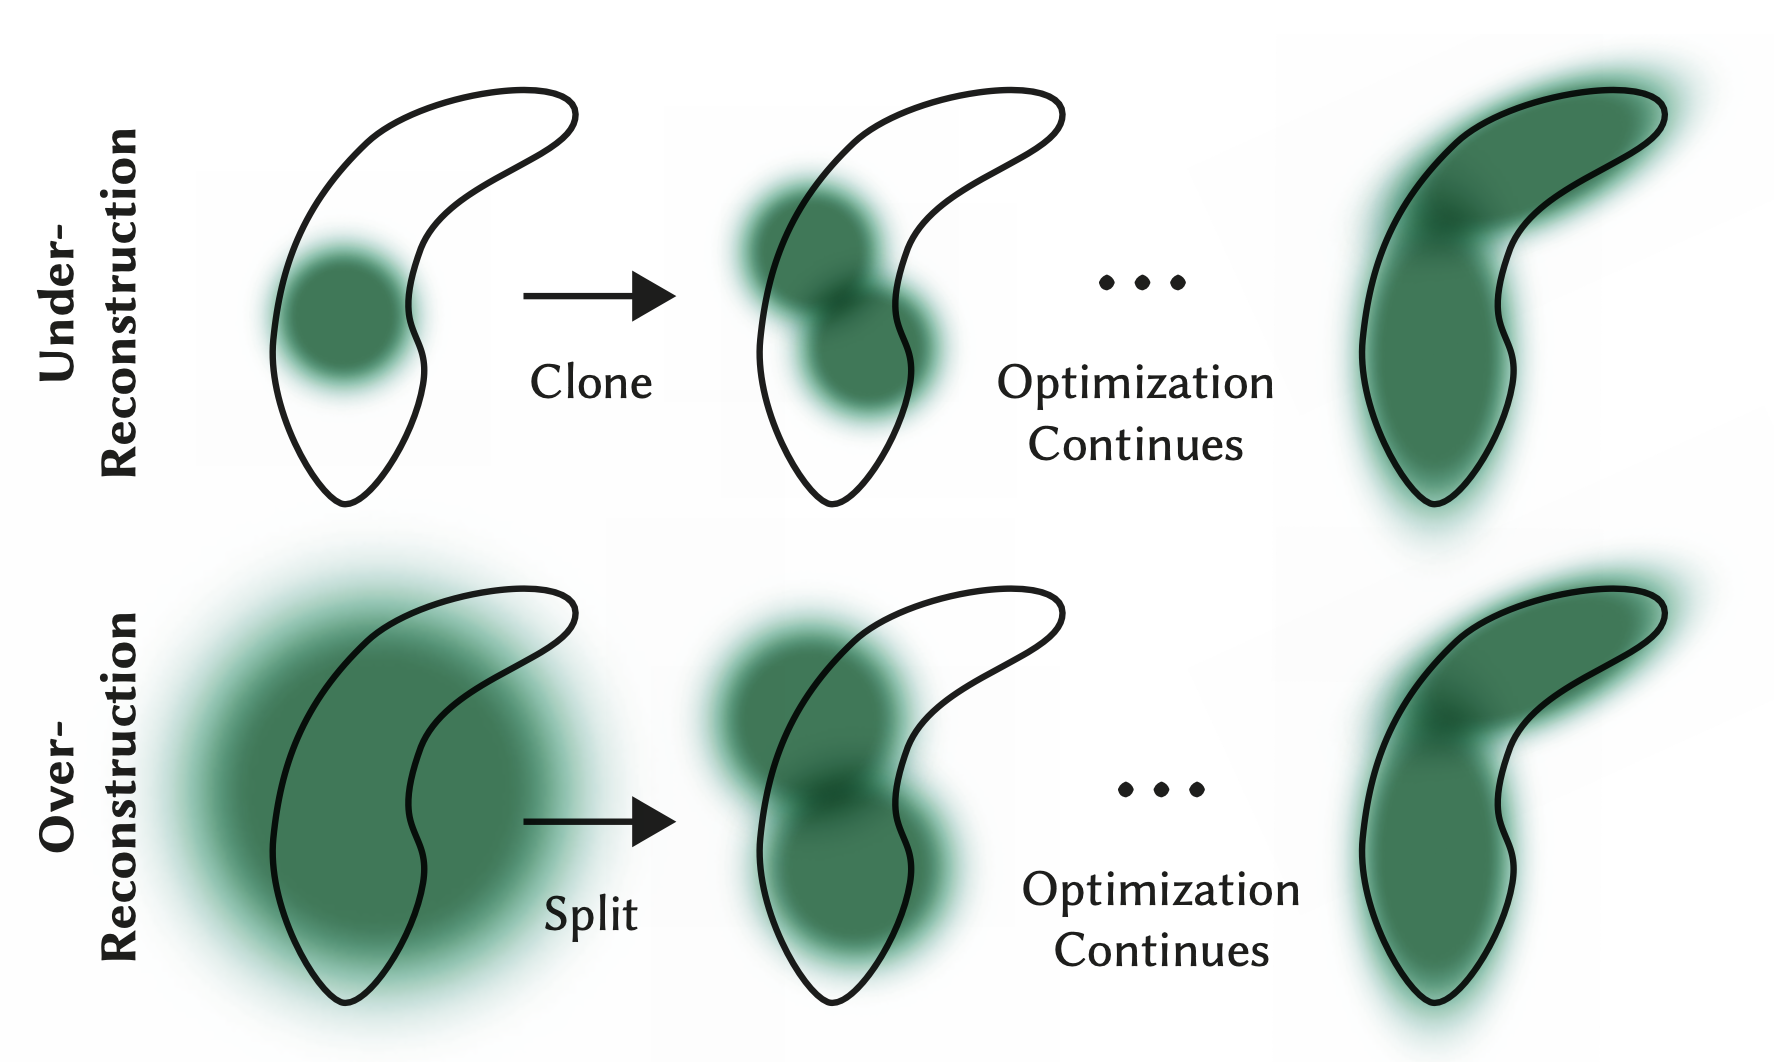
\includegraphics[width=.7\linewidth]{images/gaussiansplatting/densification-strategy.png}
\caption{\textbf{Densification Strategy.} By addressing both under and over-reconstructed areas, the densification strategy always increases the total number of gaussians but kept its associated total volume  constant in the \textit{split} stategy (contrary to the \textit{clone} one).}
\label{fig:gs-densification}
\end{figure*}



\section{Method}
\subsection{Camera path stabilization}

As we should except, COLMAP camera poses that were estimated do not describe a lean and regular trajectory around the car (Figure \ref{fig:gs-camera-path-unstab}). We thus need to correct these poses in order to describe a circular camera path around the car. 


Merging the photographs from the scene depicted on Figure \ref{fig:gs-original_scene} leads to a too bumpy result from a camera path perpective. Transition between two views are unpleasant since images of the car are inconsistent from a distance and camera look at direction perspective: Figure \ref{fig:gs-unstabilized-gif} shows how a raw and uncorrected merge of these view into a \textit{.gif} animation looks like. 

\begin{center}
  \animategraphics[autoplay,loop, poster=0,width=\linewidth]{5}{images/gaussiansplatting/gt/img-}{0}{35}
  \label{fig:gs-unstabilized-gif}
  \captionof{figure}{\textbf{Unstabilized camera path} Resulting image merge into a \textit{.gif} animation is too erratic since corresponding camera path has not been stabilized.}
\end{center}

Let's denote $\mathcal{I}=\{I_{i}\}_{i=1}^{N}$ the set of N RGB images, paired with their associated viewpoint $\pi_{i}$, and  $\mathcal{C} = \{C^{(i)}\}_{i=1}^{N}$ the set of COLMAP-based camera centers. These centers are expressed in world coordinates as: 
\begin{equation}
  C^{(i)}=-R_{i}^{T}t_{i}
\end{equation}
 where $R_{i}$ and $t_{i}$ respectivelly account for the world to camera rotation and translation. The car centroid $O_{car}$ is directly built from the 3D tires location\footnote{which are also estimated by another algorithm that would not be described in this manuscript}: 

\begin{equation}
  \begin{split}
  O_{car} = t_{RL}^{(3D)} + & \frac{t_{1}+t_{2}}{2} -(t_{1}\otimes t_{2})\frac{\left\lVert t_{r}\right\lVert_{2}}{2} \\ \\
  & t_{1} = t_{FL}^{(3D)} - t_{RL}^{(3D)} \\
  & t_{2} = t_{RR}^{(3D)} - t_{RL}^{(3D)} 
  \end{split}
  \end{equation}

where $\otimes$ denotes the cross-product and $t_{FL}^{(3D)}$ the front-left 3D tire location.\footnote{The rear-right tires is thus denoted $t_{RR}^{(3D)}$} Considering the \ac{SVD} of $\mathcal{C}_{c} = \mathcal{C} - O_{car}$, the normal $\vec{n}$ of the 2D plane that fits the best $\mathcal{C}_{c}$ is expressed as the right singular vector whose singular value is the smallest. 

[Write down proper equation for 3D projection onto the plane / 2D coordinates on the plane, circle fitting and points projections on finally points projections onto this circle]

The camera path can thus stabilized at a fixed height around circle, as describe on Figure \ref{fig:gs-camera-path-stab}. We present in Appendix \ref{appendix:spherical-interp} how sperical interpolation can be used to evenly space these camera locations around the computed circle. 


\begin{figure}[htb!]
  \centering
  \begin{subfigure}[b]{0.45\linewidth}
    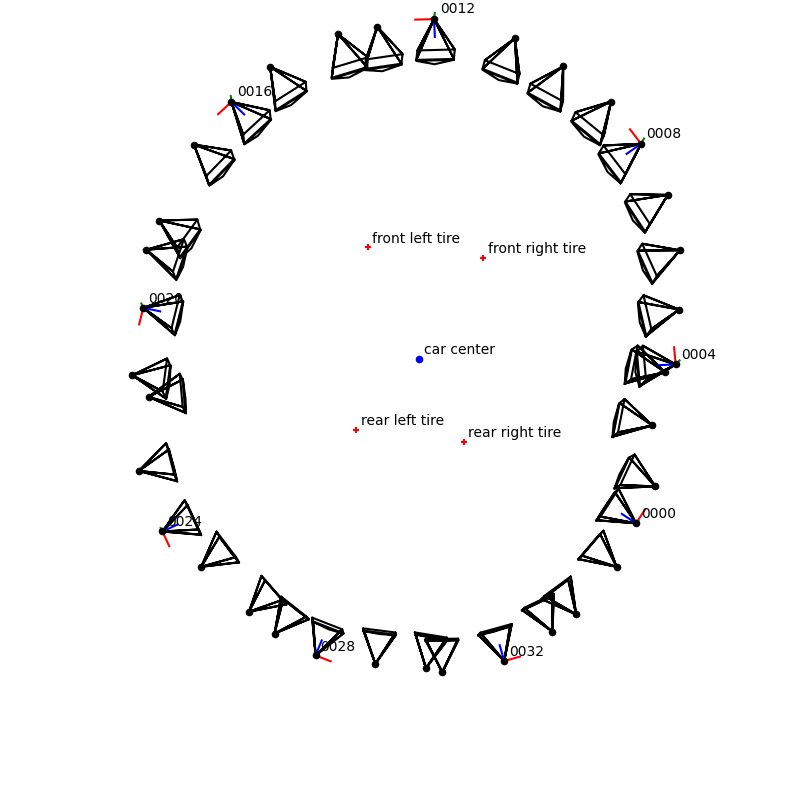
\includegraphics[width=\linewidth]{images/gaussiansplatting/camera-path-unstabilized.png}
    \caption{\textbf{Original camera path.} COLMAP predicted camera poses are unevenly spaced and do not describe a smooth path around the car. }
\label{fig:gs-camera-path-unstab}
  \end{subfigure}
  \quad % Space between the figures
  \begin{subfigure}[b]{0.45\linewidth}
    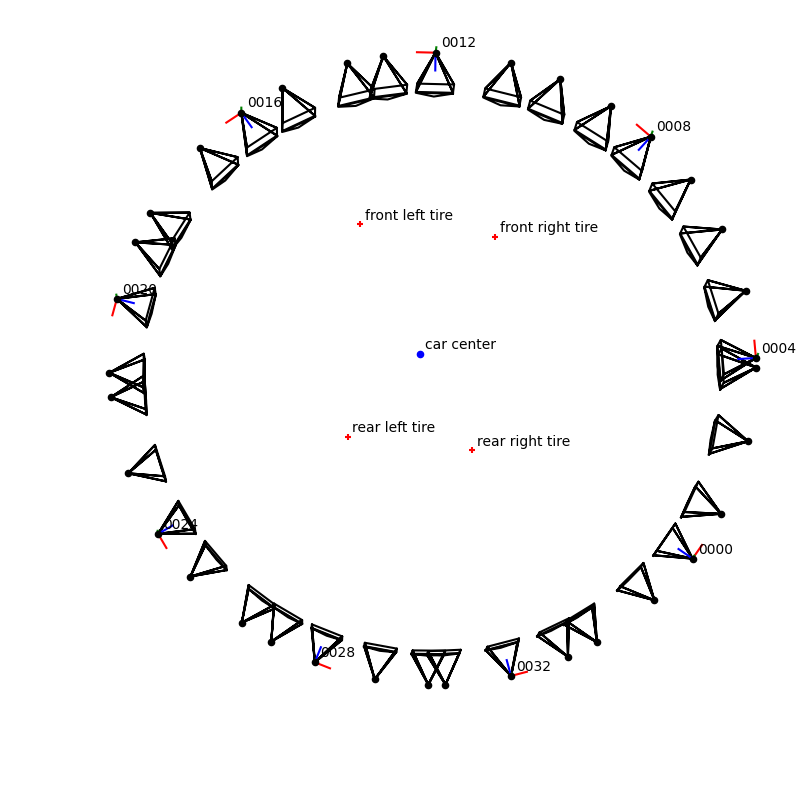
\includegraphics[width=\linewidth]{images/gaussiansplatting/camera-path-stabilized.png}
    \caption{\textbf{Corrected camera path.} Camera poses has been projected around a circle, centered around the computed car center.}
    \label{fig:gs-camera-path-stab}
  \end{subfigure}
  \caption{\textbf{Camera path set overview} Whereas camera centers have been set around a circle, they remain unevenly spaced.}
  \label{fig:gs-campath}
\end{figure}

\subsection{$360\degree$ with homography}

We present in this subsection the first and most straightforward way to obtained stabilized views from the scene: leveraging the perspective transformation theory. Indeed, such a transformation can be computed and applied to all the source views as soon as we get the orginal $\mathcal{C}$ and stabilized camera $\mathcal{C}_{stab}$ world locations. 

Given any camera center $C^{((i))}_{stab} \in \mathcal{C}_{stab}$, one can retrieve the corresponding rotation $R_{i}^{stab}$ in world coordinates through: 

\begin{equation}
  \begin{split}
    rot^{(i)}_{Z} & = - {\left[C^{((i))}_{stab}\right]}_{2}\\
    rot^{(i)}_{X} & = - e_{1} \otimes rot^{(i)}_{Z} \\
    rot^{(i)}_{Y} & = {\left[rot^{(i)}_{Z}\otimes rot^{(i)}_{X}\right]}_{2}
    \end{split}
\end{equation}
and 
\begin{equation}
R_{i}^{stab}  = \begin{bmatrix}
      rot^{(i)}_{X}\\
      rot^{(i)}_{Y} \\
      rot^{(i)}_{Z}
      \end{bmatrix}
\end{equation}

while the associated homography describing how $\pi_{i}$ moved from $C^{((i))}$ to $C^{((i))}_{stab}$ is trivially computed as: 

\begin{equation}
  \begin{split}
    H_{R}^{(i)} & = R_{i}^{stab}R_{i}^{T} \\
    H_{t}^{(i)} & = - R_{i}^{stab}(C^{((i))}_{stab} - C^{((i))})
  \end{split}
\end{equation}

The camera intrinsinc $K$ (that can also be estimated by COLMAP) enables, with $H^{(i)}$, to apply a perspective transformation on the corresponding view. We present on the Figure \ref{fig:gs-homography-view3} how the view index \textit{0003} has been transformed. 

\begin{figure}[htb!]
  \centering
  \begin{subfigure}[b]{0.45\linewidth}
    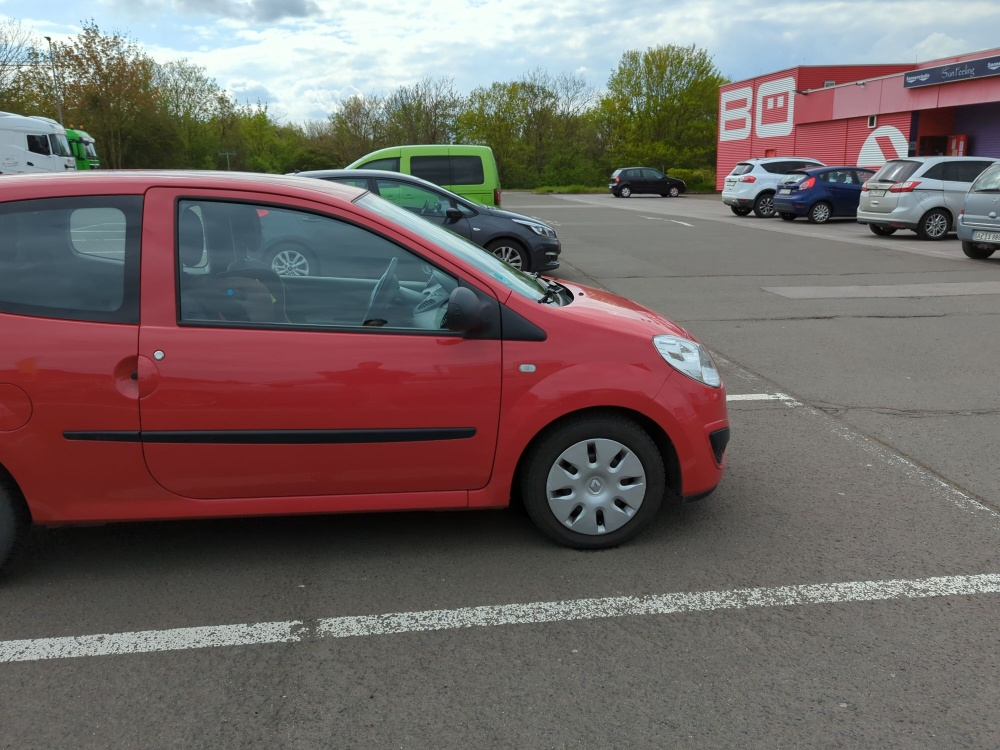
\includegraphics[width=\linewidth]{images/gaussiansplatting/gt/img-3.jpg}
    \caption{\textbf{Original view.}}
    \label{fig:view3}
  \end{subfigure}
  \quad % Space between the figures
  \begin{subfigure}[b]{0.45\linewidth}
    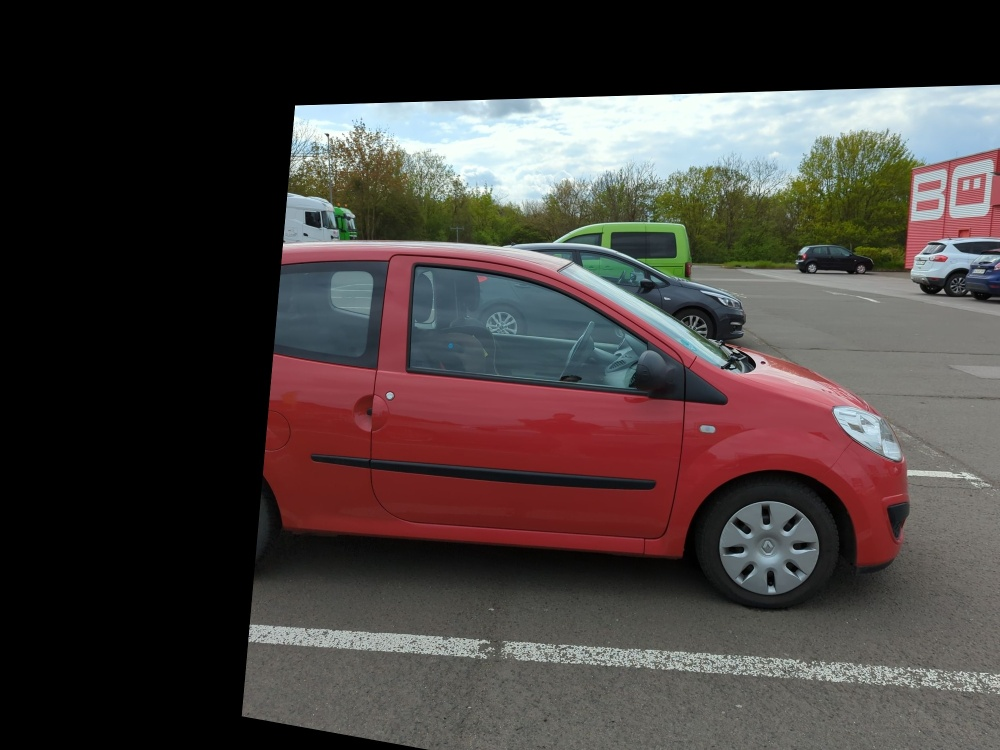
\includegraphics[width=\linewidth]{images/gaussiansplatting/stabhomo/img-3.jpg}
    \caption{\textbf{Perspective wrapped view.}}
    \label{fig:gs-view3-homo}
  \end{subfigure}
  \caption{\textbf{Perspective transformation based stabilization}. Whereas the car is now properly centered on the view, the car is cropped as the perspective transformation to apply was too drastic}
  \label{fig:gs-homography-view3}
\end{figure}

Once such transformation has been applied to the entire scene, the $360\degree$ spin tour is now properly stabilized and the corresponding animation cleaner than before, as shown on Figure \ref{fig:gs-stabilized-homo-gif}. 

\begin{center}
  \animategraphics[autoplay,loop, poster=0,width=\linewidth]{5}{images/gaussiansplatting/stabhomo/img-}{0}{35}
  \label{fig:gs-stabilized-homo-gif}
  \captionof{figure}{\textbf{Stabilized $360\degree$ spin path} The scene is now properly stabilized even though some perspective transformed views cropped the car.}
\end{center}

Car cropping is one the main limitation of this first solution and it cannot be triavially adressed. Besides, CarCutter clients often lack room to back up further when they shoot a car. There are therefore two causes that might lead to car cropping as any input view might also partially depict the car. Such a pure geometrical-based solution cannot fake or generate cars missing parts. 

\subsection{$360\degree$ with Gaussian Splatting}
\label{subsec:gs-vanilla_gs}
We investigate in this section the seminal work from \citep{kerbl20233d} on our scene. From a number of input views perspective, our scene might be considered as sparsed: research datasets used to train and test \ac{GS} often have hundreads of photographs. Since our scene is made of only 36 views, we used all of them to train the \ac{GS} model. 

We first present on the Figure \ref{fig:gs-view3} the rendering of the view indexed \textit{0003}, that was thus in the training set. As the entire 3D scene structure has been learned and is explicitly stored as a gaussian point cloud, one can render it at any locations and synthesize the whole car. 

\begin{figure}[htb!]
  \centering
  \begin{subfigure}[b]{0.45\linewidth}
    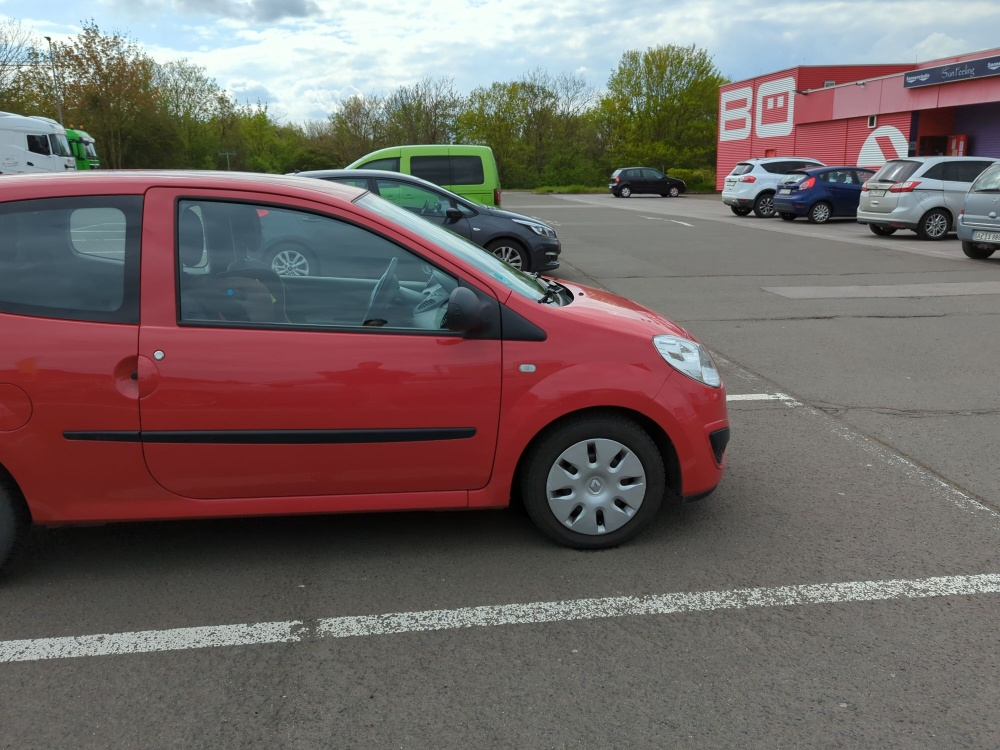
\includegraphics[width=\linewidth]{images/gaussiansplatting/gt/img-3.jpg}
    \caption{\textbf{Original view.}}
    \label{fig:view3}
  \end{subfigure}
  \quad % Space between the figures
  \begin{subfigure}[b]{0.45\linewidth}
    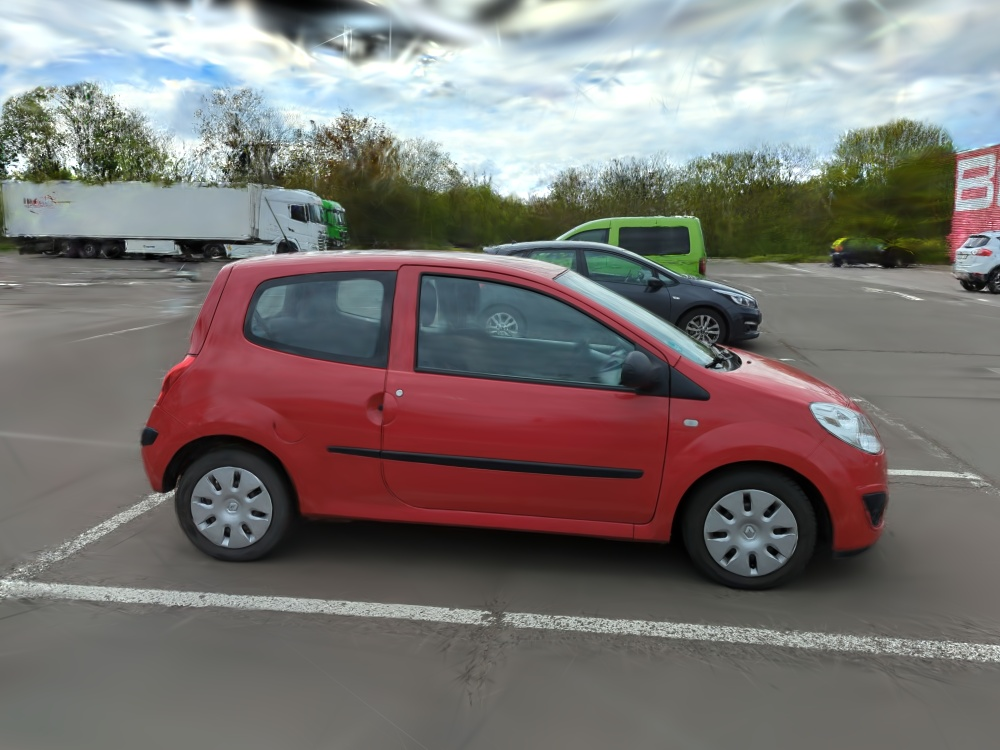
\includegraphics[width=\linewidth]{images/gaussiansplatting/stabgs/img-3.jpg}
    \caption{\textbf{Rendered view from GS scene.}}
    \label{fig:gs-view3-gs}
  \end{subfigure}
  \caption{\textbf{Gaussian Splatting based stabilization} Contrary to the homography-based solution, our trained GS is able to render the whole car.}
  \label{fig:gs-view3}
\end{figure}

The corresponding spin stabilized animation is proposed on Figure \ref{fig:gs-stabilized-gs-gif}. 

\begin{center}
  \animategraphics[autoplay,loop, poster=0,width=\linewidth]{5}{images/gaussiansplatting/stabgs/img-}{0}{35}
  \label{fig:gs-stabilized-gs-gif}
  \captionof{figure}{\textbf{Stabilized $360\degree$ spin path with GS} Whereas the car is not cropped anymore during stabilization, some details are missing on the car.}
\end{center}

The scene we considered is not prone to such undesired effect but it might occur during rendering that floaters artifacts appear. As we stabilize the camera path and render views at locations that were not originally observed, these artifacts are actually not very surprising. There floaters must be removed directly from the 3D scene itself, so that they are not render. We chose first, before delving into a floater removal algorithm, to slighly change minimal depth distance of the culling frutrum. Figures \ref{fig:gs-cullingfrustrum} and \ref{fig:gs-floaters} respectivelly present the core idea of such modification and its direct impact during rendering on an other scene (since the original one does not have such visible floaters). 


\begin{figure*}[htb!]
  \center
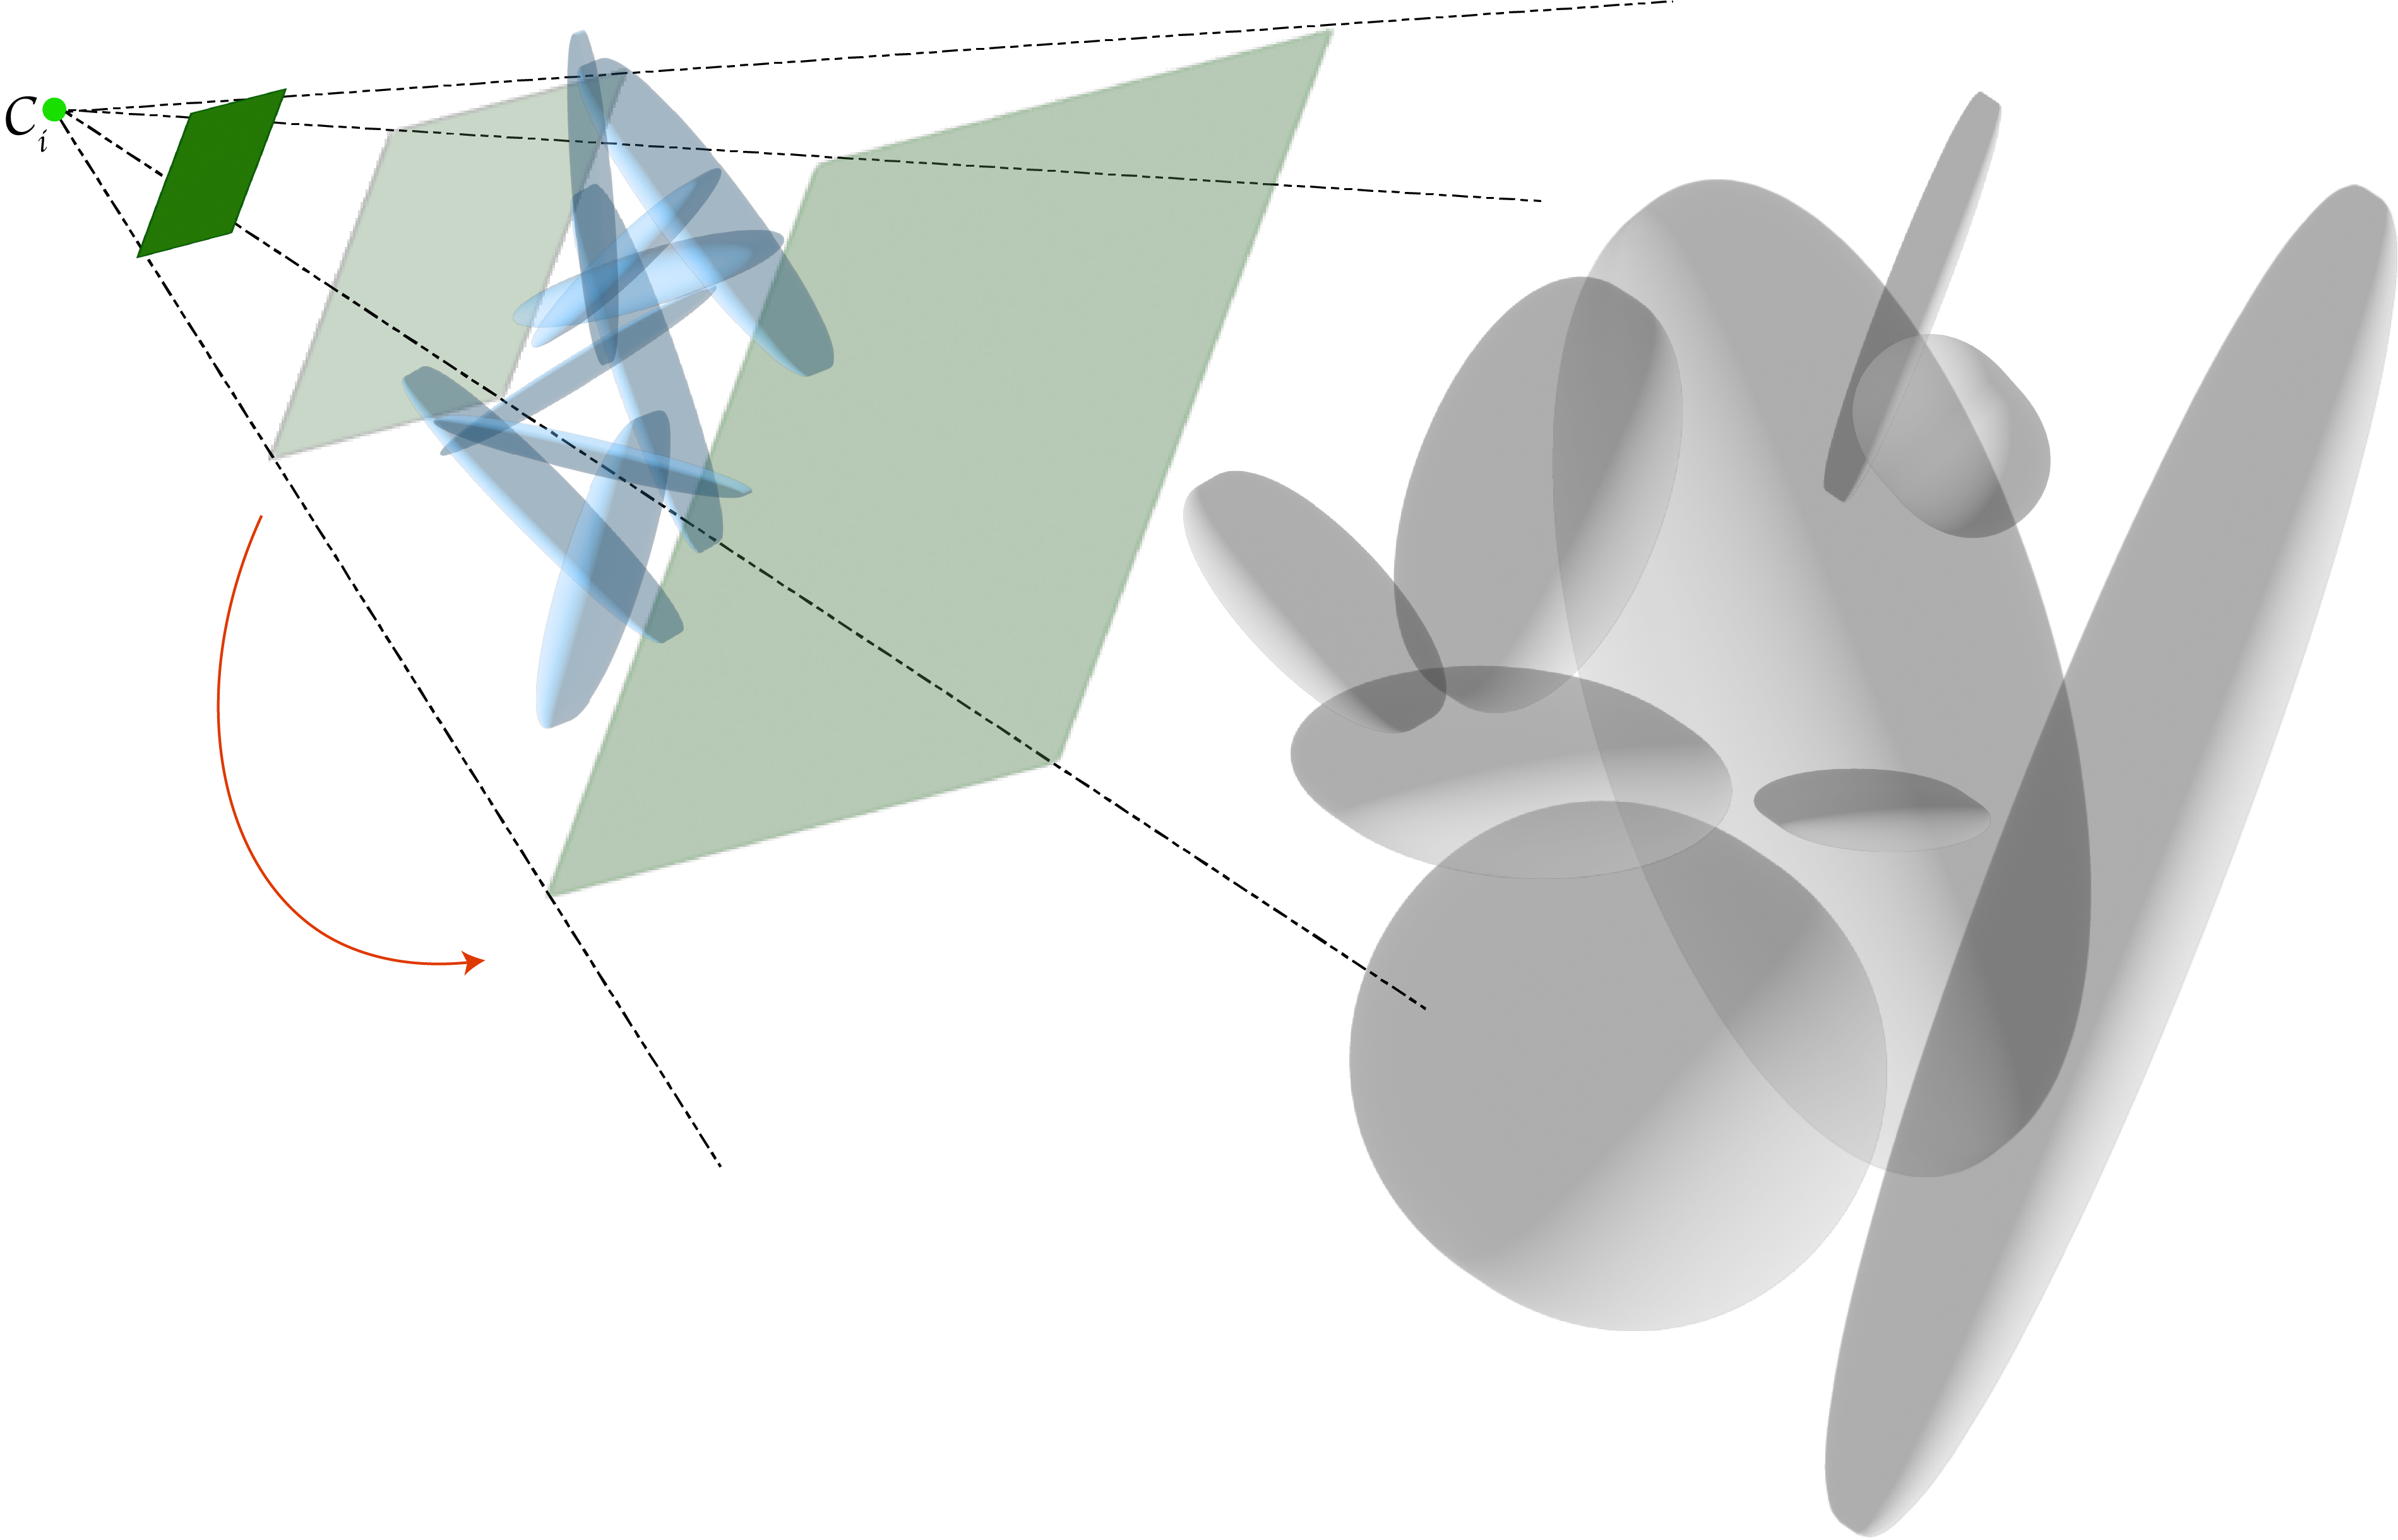
\includegraphics[width=.7\linewidth]{images/gaussiansplatting/gaussian-floaters.png}
\caption{\textbf{Floater artifacts visualization} Moving the minimal depth distance from which a gaussian fall into the culling frustrum enables to avoid rendering floaters. Such floaters are often non observable at training locations since they lie behind the camera.}
\label{fig:gs-cullingfrustrum}
\end{figure*}

The stabilization of the scene on Figure \ref{fig:gs-floaters} induced a small step back. Such a minor camera displacement has caused some floating gaussians to fall into the culling frustrum of this new position, and have thus been rendered. Restrict a bit the culling frustrum to avoid too closed gaussians to be rendered allow to easely get ride of them. 
 
\begin{figure*}[htb!]
  \center
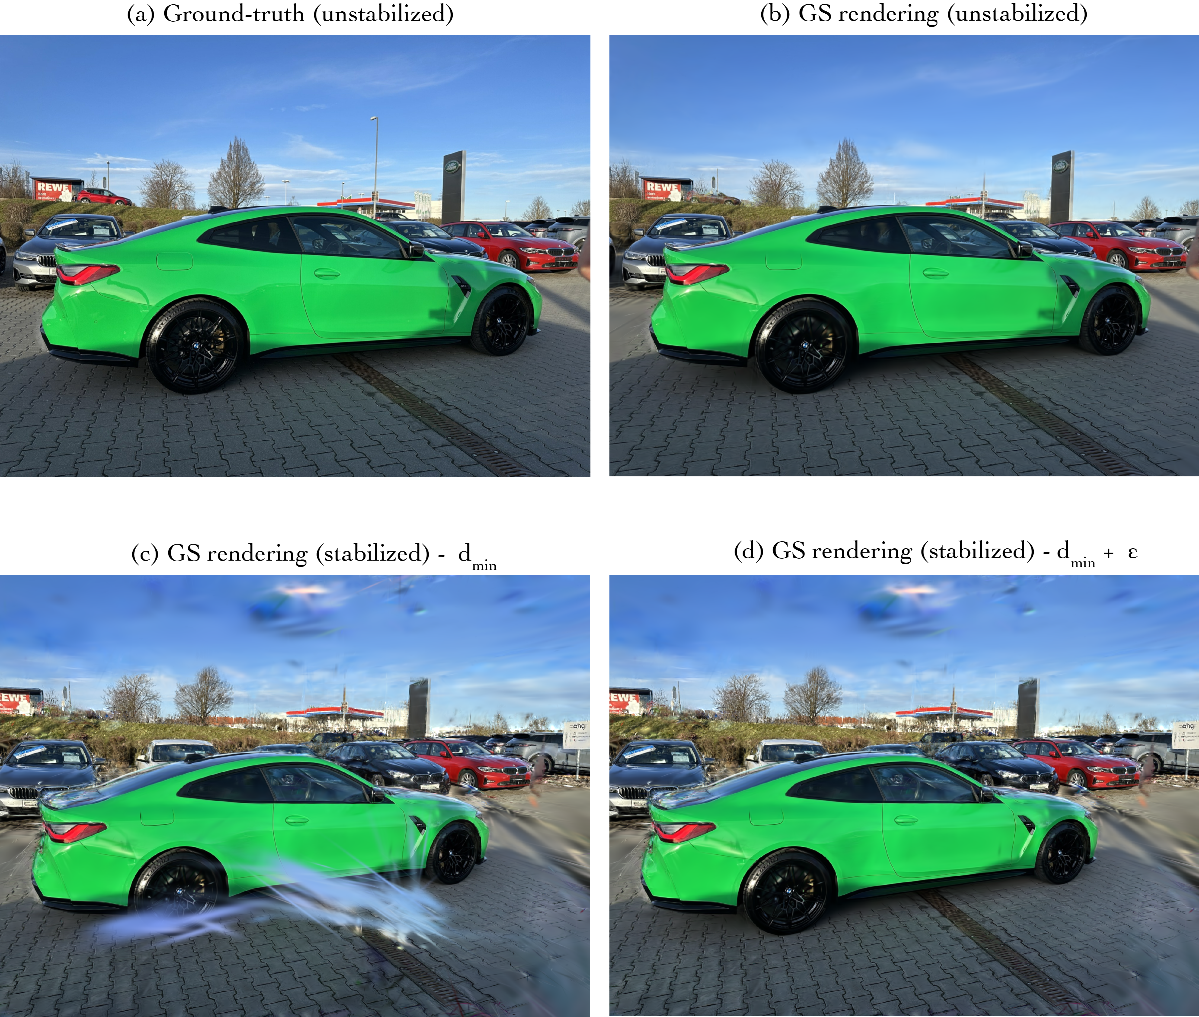
\includegraphics[width=.7\linewidth]{images/gaussiansplatting/gaussian-floaters-results.png}
\caption{\textbf{Floater artifacts rendering} Render the scene at training (unstabilized) locations does not induce any floater artifacts (see \textit{(b)}). However, once the scene is stabilized and the corresponding view rendered, small \textit{needle} artifact appear. Setting a higher minimal distance for a gaussian to fall into the culling frustrum allow to get ride of these floaters.}
\label{fig:gs-floaters}
\end{figure*}



\section{Experiments}
\ref{sec:gs-experiment}

\subsection{View-dependancy effect}

\subsection{Visual Hull}
We experiment in this section a novel way to get the initial point cloud $\mathcal{P}$ we need to start with for \ac{GS} training. As it has already been shown on Figure \ref{fig:gs-sfm} and explained in \ref{subsec:gs-sfm}, the point cloud COLMAP produces is extremely sparse: $\mathcal{P}$ has only roughly 4K points and most of them do not lie on the car surface. 

We consider a novel point cloud, termed $\mathcal{P}_{VH}$, that direclty leverages from a visual hull, a silhouette-from-motion based-concept. The main idea is rather straightforward, since it only requires to get the posed images and the corresponding binary masks. The Figure \ref{fig:gs-vh-concept} allows to grasp the visual hull concept. 

\begin{figure*}[htb!]
  \center
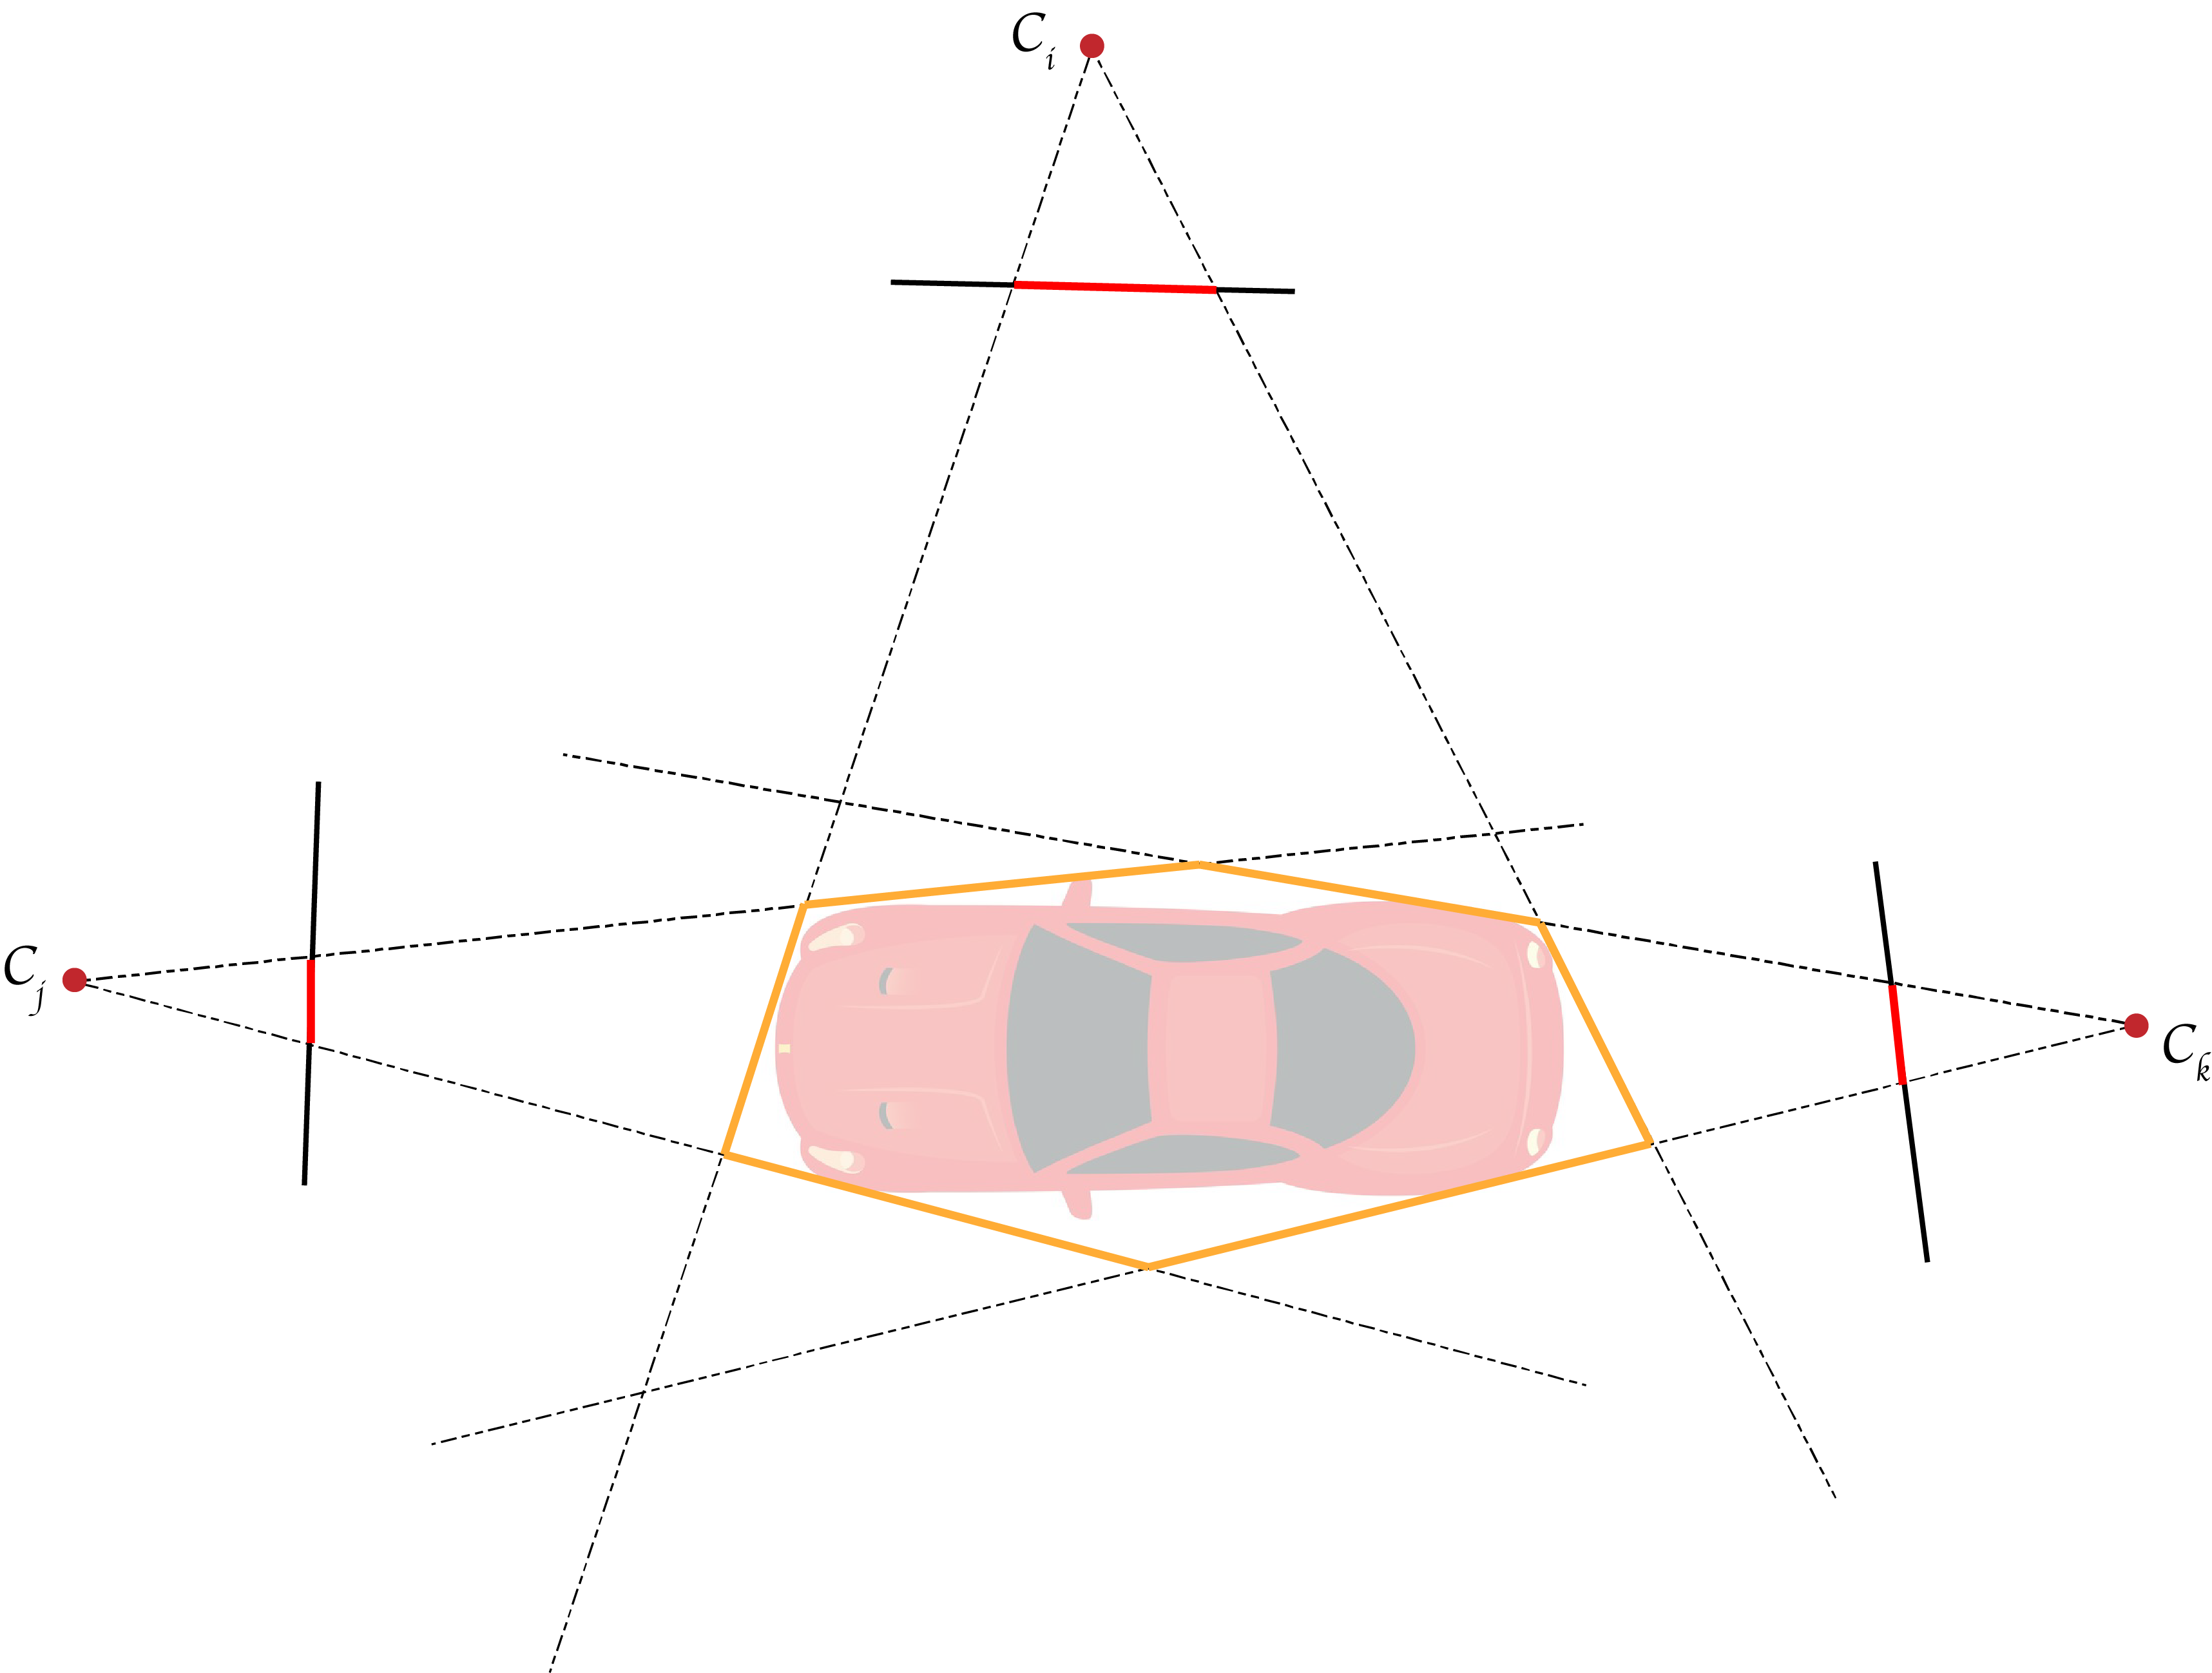
\includegraphics[width=.7\linewidth]{images/gaussiansplatting/visualhull-idea.png}
\caption{\textbf{Visual hull concept.} A visual hull is here built as the intersection of three 3D bounding cones from the silhouette masks. Such hull is almost convex in case of our car scenario. One can  sample 3D points within the visual hull to build a new dense point cloud.}
\label{fig:gs-vh-concept}
\end{figure*}

We present on Algorithm \ref{alg:gs-vh} the pseudo code that allow to generate such a visual hull and the corresponding dense coloured point cloud $\mathcal{P}_{VH}$ we can obtained on Figure \ref{fig:gs-vh-result}. 

\begin{algorithm}[h]
  \caption{Visual hull contruction}\label{alg:gs-vh}
  \SetKwInOut{Input}{input}
  \SetKwInOut{Output}{output}
  \SetKwInOut{Parameter}{parameter}
  \Input{Images $\mathcal{I}$, Silhouette mask $\mathcal{S}$}
  \Parameter{Intrinsic and extrinsic camera parameters $\pi=K[R|t]$}
  \Output{Visual hull-based point cloud $\mathcal{P}_{VH}$ } 
  \medskip
  \KwResult{$\mathcal{P}_{VH}$ can be densely sampled}
  \medskip
  $bbox \gets \mathbf{build3DBB}()$ \tcp*[l]{Create a vanilla 3D bounding boxe}
  $P_{3D} \gets \mathbf{sampleDensely}(bbox)$\hspace{.4cm}\textcolor{gray!80}{\# 
    [$N_{pts}$,3]} \tcp*[l]{Sample points in the BB}

   $P_{2D} \gets \mathbf{project}(P_{3D},\pi)$ \hspace{.4cm}\textcolor{gray!80}{\# 
    [$N_{pts}$,2]} \tcp*[l]{Reproject on image plane }
    
    $idx_{valid} \gets \mathbf{keepValidPoints}(P_{2D},\mathcal{M})$ \hspace{.4cm}\textcolor{gray!80}{\# 
    [$N_{pts}$,1]} \tcp*[l]{Boolean. 1 if valid, 0 otherwise}

    $P_{3D}^{(refined)} \gets P_{3D}[idx_{valid}]$ 

    $P_{VH} \gets \mathbf{setRGBcolor}(P_{3D}^{(refined)},P_{2D},idx_{valid},\mathcal{I})$ \tcp*[l]{Set RGB color to the point cloud through bilinear interpolation}
\end{algorithm}


\begin{figure*}[htb!]
  \center
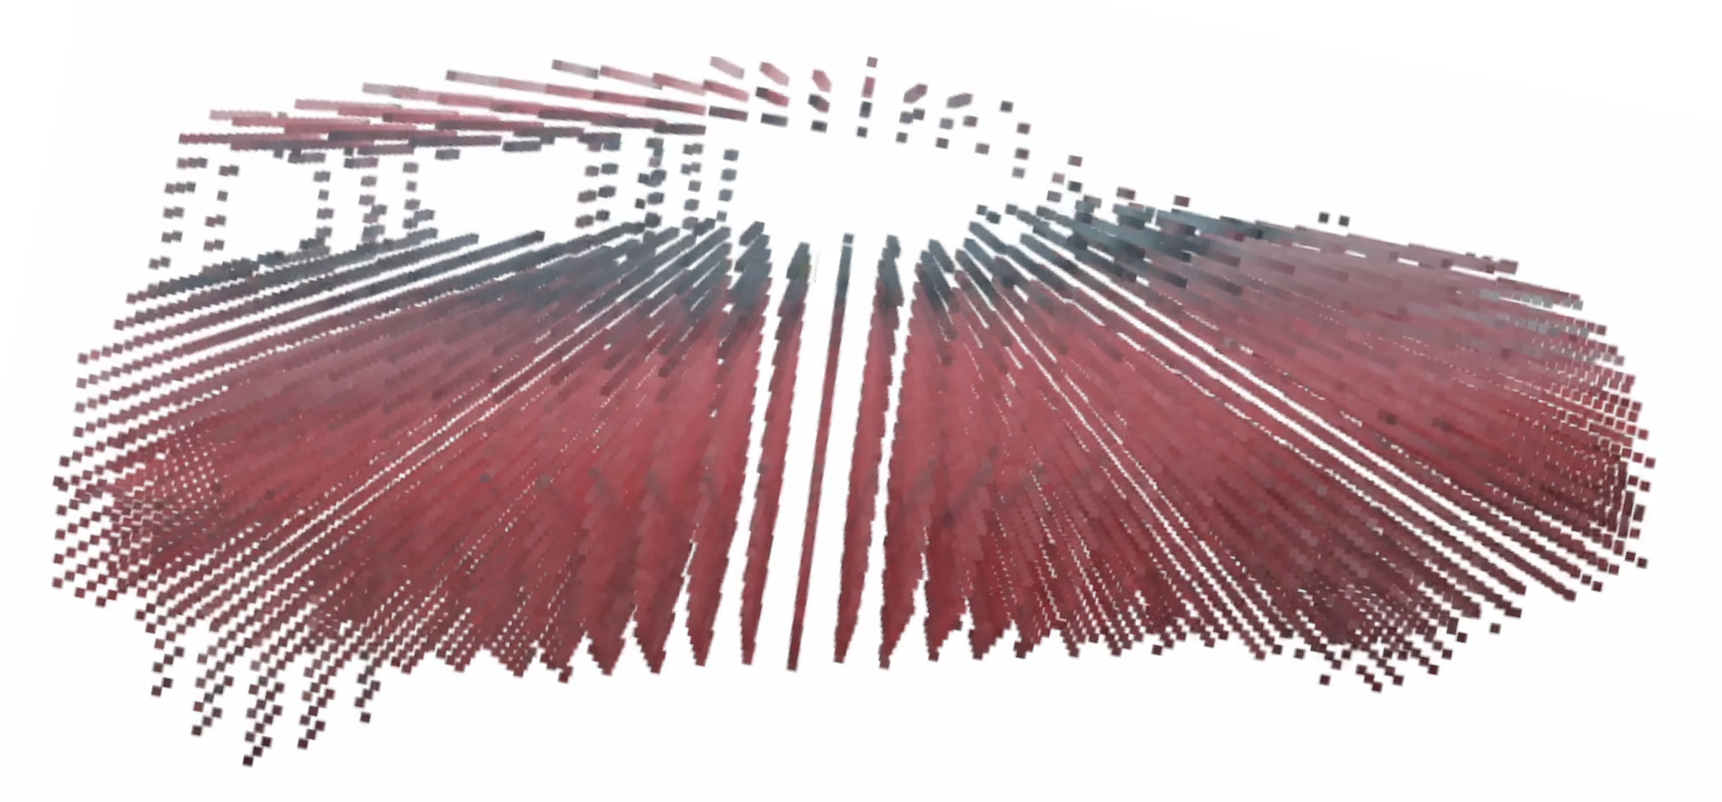
\includegraphics[width=.7\linewidth]{images/gaussiansplatting/visualhull-res.png}
\caption{\textbf{Visual hull concept.} A visual hull is here built as the intersection of three 3D bounding cones from the silhouette masks. Such hull is almost convex in case of our car scenario. One can  sample 3D points within the visual hull to build a new dense point cloud.}
\label{fig:gs-vh-result}
\end{figure*}

However, the visual hull-based point cloud also remains incomplete in its current form since it leaves a large number of areas without any points in the 3D scene: sky, ground or surrounding cars are not represented by any gaussians when the \ac{GS} training starts. Even though the optimization process move some of these gaussians toward these under-reconstructed areas, the final point cloud is too sparsely densified outside of the car itself. It might not be an issue as soon as we extensively want to reconstruct and synthesize novel views of the car. Since we performing neural rendering on an explicit gaussian point-clouds, undesired gaussians (such as these needle floaters artifact described on Figure \ref{fig:gs-floaters}) might be rasterized \textit{over} the car.  

One naive yet effective solution is thus to merge the two original point cloud we have at our disposal: $\mathcal{P} = \mathcal{P}_{COLMAP} \cup \mathcal{P}_{VH}$. We therefore expect to benefit from the higher point density of $\mathcal{P}_{VH}$ on the car and from the better background representation of $\mathcal{P}_{COLMAP}$ too. Whereas it increases the original volume of gaussians to optimize, and thus the training time, rendering at stabilized locations are more visually pleasant, with better car inner details synthesis. The figure \ref{fig:gs-vishull-comp} and Table \ref{table:gs-vh-influence} both visually and quantitatively confirm the benefit of this point cloud merging strategy. 

\begin{figure*}[htb!]
  \center
\includegraphics[width=.9\linewidth]{images/gaussiansplatting/vishull-comp.png}
\caption{\textbf{Point cloud initilization influence.} COLMAP-based point \textit{(left)} cloud yields a satisfying result, even though some inner details are missed. The visual hull based \textit{(center)} initialization method produce sharper results in the car, but floaters are rendered on the roof the car. Merging the two point cloud \textit{(right)} allows to get the best of both configuration.}
\label{fig:gs-vishull-comp}
\end{figure*}


\begin{table}[htp!]
  \caption{\textbf{VisualHull influence} Quantitative results how influenciable the original point cloud can be on the GS rendering performance.}
  \label{table:gs-vh-influence}
  \centering%\begin{center}
  \begin{adjustbox}{width=\linewidth}
  \begin{tabular}[h]{c||ccccccc}
  \hline
   PC initialization & \multicolumn{3}{c}{Full Image} & \multicolumn{3}{c}{Car only} \\
   &  SSIM ($\uparrow$) & PSNR ($\uparrow$) & LPIPS ($\downarrow$) & SSIM ($\uparrow$) & PSNR ($\uparrow$)) & LPIPS ($\downarrow$)\\
  \hline
  COLMAP-SfM  & 0.787  & 28.592 & 0.334 & 0.990 & 41.998 & 0.020 \\
  VisualHull & 0.736 & 26.850 & 0.392 & 0.990 & 41.835  & 0.018 \\
  COLMAP-SfM + VisualHull & \cellcolor{red!25}0.810 & \cellcolor{red!25}29.288 & \cellcolor{red!25}0.314 & \cellcolor{red!25}0.993 & \cellcolor{red!25}43.452  & \cellcolor{red!25}0.014 \\
  \hline 
  \end{tabular}
  \end{adjustbox}
  %\end{center}
  \end{table}

\subsection{Revisiting the ADC strategy}

As \citep{zhang2024pixel}

\section{Conclusion}

\cleardoublepage
\let\leftmark=\oldleftmark

\acresetall
\chapter{Conclusion}
\label{chapter:conclusion}

%\minitoc
\chapterwithfigures{\nameref*{chapter:conclusion}}
%\chapterwithtables{\nameref*{chapter:introduction}}

\ifthenelse{\boolean{skipConclusion}}{\endinput}{}

This thesis primarely focused on the novel view synthesis issue, mostly with the highly constrained single-view scenario. We skim through in this section over our core contributions, before drawing up  the current 2024 landscape in \ac{IA} and 3D. The last section of this manuscript will be devoted to the perspectives and further work this PhD thesis might lead to. 

\section{Contributions}

This manuscript has adressed in a large extend the single-image \ac{NVS} issue. We built in our first two contributions around latest deep learning architectures to synthesize a novel viewpoint of a static scene from a single source posed image. Our latest project has an industrial primary aim, where novel views are rendered from a scene that was explicitly reconstructed in 3D as a gaussian point cloud.

We started this manuscript by presenting in Chapter \ref{chapter:epipolarnvs} our epipolarNVS architecture. Our main motivation through this work was to propose an innovative way to encode camera pose information in an image-to-image \ac{CNN} for \ac{NVS}. Whereas most of prior work often discretized \citep{kim2020novel} or encoded camera pose information into a low dimensional signal \citep{sun2018multiview}, we rather exploited the epipolar constraint to encode such prior signal. Through a vanilla grid sampling strategy on the source view, we project epipolar lines on a blank RGB image, that was been fed alongside the source image to pose-condition the network. 

We then investigated in Chapter \ref{chapter:epinerf} how epipolar constraints could be bring into a generalizable \ac{NeRF} architecture for single-image \ac{NVS}. Based on \textit{source-aligned} dense feature volume produced from a CNN-encoder, we trained a novel \ac{NeRF}-architecture, termed NeRFeature \ref{subsec:epinerf/method/nerfeature} to produce \textit{target-aligned} features. These \textit{source} and \textit{target-aligned} feature are finally used through an epipolar constraint in a light attention mechanism. We extensively shown in the devoted Experiments section \ref{subsec:epinerf/experiments} how our three-stage training architecture might help generalizable \ac{NeRF}s to better perfrom on single-image \ac{NVS} task.  

Finally, Chapter \ref{chapter:gausssplat} has been entirely devoted to the \ac{NVS} solution we started investigated with CarCutter by Meero few months ago. The camera spin stabilization algorithm allows to render from a 3D \ac{GS} reconstructed scene novel viewpoints which were initially uncomplete and cropped (subsection \ref{subsec:gs-vanilla_gs}). We presented a bunch of improvements to go beyond this first reconstruction in Experiments \ref{sec:gs-experiment}. However, 3D \ac{GS}-based scenes remain prone to floaters artifact when they are rendered at non-training locations. We will push in that direction in a close future to develop a floater removal algorithm. While results are still unperfect for an industrial application, research and open-source projects around \ac{GS} \citep{kerbl20233d} are tremendously prolific and move at a very steady pace for 10 months now \citep{luiten2023dynamic,yang2024gaussianobject,wewer24latentsplat}. 

On top of these contributions, we also introduce in Appendix \ref{chapter:appendix} our very first work, called AdaptativeSR \citep{landreau2022adaptativesr}. There is no direct relationship with the \ac{NVS} but rather with topological considerations in low-resolution 3D meshe structure. Idea was to leverage on the very first differentiable rasterizers that emerged in 2020 \cite{liu2019soft} (before this PhD started) to prune faces of a genus-0 object mesh. By solely relying on 2D binary rendered silhouette mask of such a 3D object, we proposed an effective yet imperfect algorithm to adapt mesh topology. 

\section{3D and IA in 2024}
\subsection{Open-source and environmental issue}
\subsection{Fundation models in 3D}
\subsection{Trends and application in 3D}
\section{Perspectives and further work}


\cleardoublepage
\let\leftmark=\oldleftmark

{
	\backmatter
	\renewcommand{\leftmark}{\spacedlowsmallcaps{\bibname}}
\renewcommand{\rightmark}{\spacedlowsmallcaps{\bibname}}

\refstepcounter{dummy}
\addtocontents{toc}{\protect\vspace{\beforebibskip}} % to have the bib a bit from the rest in the toc
\addcontentsline{toc}{chapter}{\tocEntry{\bibname}}
\printbibliography
	\cleardoublepage
	}


\appendix
\acresetall
\chapter{Appendix}
\label{chapter:appendix}

%\minitoc
\chapterwithfigures{\nameref*{chapter:appendix}}
%\chapterwithtables{\nameref*{chapter:introduction}}

\ifthenelse{\boolean{skipAppendix}}{\endinput}{}

\section{Gaussian Splatting}
\subsection{Spherical Harmonics: Definition and construction}
\label{appendix:gs-sh}

\section{AdaptativeSR}

\subsection{Introduction}
\label{sec:intro}
%%%%%%%%%%%%%%%%%%%%%%%%%%%%

%%%%%%%%%%%%%%%%%%%%%%%%%%%%
The image-based 3D reconstruction task aims at building a 3D representation of a given object depicted onto a natural or synthetic set of images. Human being learned from an early age to apprehend their surrounding 3D environment and thus have high cognitive abilities for mentally inferring a 3D scene from a single 2D image. Such a task is way more challenging in computer vision since there are no manners for a 2D image to lossless embrace the information contained in an entire 3D scene. While image-based 3D reconstruction is approached for decades in computer vision and graphics with robust and renowned techniques such as Structure-from-Motion \citep{longuet1981computer}, the latest learning-based approaches address the problem through a new prism by making extensive use of deep neural networks
\citep{kanazawa2018learning,deng2019accurate,saito2020pifuhd}.

%%%%%%%%%%%%%%%%%%%%%%%%%%%%%%
The single-image based 3D reconstruction issue even brings the challenge one step above as inputs are more constrained. From a general perspective, the latest contributions related to single-image 3D reconstruction chose to work with mesh structures rather than 3D point clouds or voxel grids, since they offer a well-balanced trade-off between computational requirements and tiny 3D details retrieving. Meshes also embed a notion of connectivity between vertices, contrary to the point cloud representation where such valuable property is missing.

%%%%%%%%%%%%%%%%%%%%%%%%%%%%%
The rendering operation somehow fills the gap between the 3D world and the 2D image plane by mimicking the optical image formation process. Such procedure is widely well known in graphics, but it has been brought into computer vision learning-based approaches for only a few years now for a significant reason: the rasterization stage involved in any rendering process is intrinsically non-differentiable since it requires a face selection step. It recently led to self-supervised single-image 3D reconstruction methods where 3D ground truth labels are thus no more needed.
%%%%%%%%%%%%%%%%%%%%%%%%%%%%%%%%%%%%%%%%%%

Changing the topology during the 3D mesh reconstruction process can mainly be done in two ways: either by pruning some edges/faces or by adding edges/vertice to generate new faces onto the mesh surface. Single-image 3D reconstruction methods that require 3D supervision already apply these techniques in their training pipeline\citep{pan2019deep,nie2020total3dunderstanding,smith2019geometrics}. However, most of the current state of the art methods in self-supervised single-image 3D reconstruction -where 3D labels are thus no more needed- perform mesh reconstruction with a roughly similar approach. An Encoder-Decoder network iteratively learns to predict an elementary per-vertex displacement on a 3D template sphere to reconstruct as faithfully as possible a 3D mesh associated with the provided input images. This strategy only affects the geometry of the mesh and thus do not get consideration for its topology. Indeed, vertice position impacts edges length and dihedral face angles but let the overall topology unchanged. These topological considerations, yet fundamental when embracing 3D mesh structures, are often bypassed in the current self-supervised single image-based 3D reconstruction literature. We thus claim that the latest advances in differentiable rendering \citep{liu2019soft,ravi2020accelarating} are informative enough to address this fundamental concept.
%%%%%%%%%%%%%%%%%%%%%%%%%%%%%%%%%%

This paper thus brings topological considerations into the self-supervised image-based 3D reconstruction framework. The core idea of our work is to leverage onto the differentiable renderer from \citep{ravi2020accelarating} to detect the potential faces/edges to prune onto the mesh without leveraging onto 3D supervision, as made in \citep{pan2019deep,nie2020total3dunderstanding,smith2019geometrics}. To the best of our knowledge, no attempts have been made in this direction. Our work is thus in line with self-supervised image-based 3D reconstruction methods, even though our topological refinement module is agnostic to the mesh reconstruction network used. Our contribution is summarised through: 
\begin{itemize}
    
    \item A fast and efficient strategy to prune faces onto a 3D mesh by only leveraging 2D alpha masks and camera pose. 

    \item A topological refinement module that is agnostic to the 3D mesh reconstruction network.
\end{itemize}

%%%%%%%%%%%%%%%%%%%%%%%%
\subsection{Related works}
\label{sec:related_works}
%%%%%%%%%%%%%%%%%%%%%%%%%

Issues presented in this section are the closest ones related to our work. \newline 

\noindent\textbf{Differentiable renderer} OpenDR \citep{loper2014opendr} is one of the first differentiable renderers and therefore paved the way in this line of work in 2014. However, the differentiable rendering issue has gained interest over the past few years. The significant progress that has been achieved in this direction since 2017 tend to prove such a trend. Hiroharu Kato \etal introduced an approximate gradient strategy with NMR\citep{kato2018neural} while SoftRasterizer\citep{liu2019soft} proposed a truly differentiable framework without gradient approximation through a probability-distance based formulation. Wenzheng Chen \etal designed their differentiable renderer with foreground-background pixel consideration in their DIB-R \citep{chen2019learning} method. Whereas an interpolation-based formulation gives foreground pixels value, background ones are predicted through the same probability maps aggregation as used in \citep{liu2019soft}. These three differentiable frameworks are the most used ones in the latest self-supervised single-image 3D reconstruction methods \citep{kanazawa2018learning,li2020self,pavllo2020convolutional}. While PyTorch3D \citep{ravi2020accelarating} is extremely powerful from a computational point of view, it has been released too recently and has not yet given rise to new contributions in self-supervised 3D reconstruction. In addition to these renderers that are thus primarily designed to work with mesh structures, other types of renderers\citep{niemeyer2020differentiable,jiang2020sdfdiff} also emerged few years ago to address the rendering of 3D shapes parametrized through implicit surfaces. 

\noindent\textbf{Single Image-based 3D Reconstruction} First works related to the single image-based 3D reconstruction issue in a deep learning framework \citep{choy20163d,girdhar2016learning,yang2018dense} make extensive use of 3D datasets \citep{chang2015shapenet,sun2018pix3d} since the mesh generation network is entirely supervised through 3D ground truth labels. These methods entirely missed out on the physical image formation process during training since there is no need to consider it as soon as 3D labels are accessible. In this way, existing 3D loss functions are sufficient to predict feasible 3D mesh structures from a 3D sphere template. While a tremendous number of works have leveraged over 3D labels, the current trend in single image-based 3D reconstruction instead tries to capitalise onto differentiable renderers and thus limit as much as possible the need for an expensive 3D supervision. It leads over the last few years to a new line of work called self-supervised image-based 3D reconstruction  \citep{kanazawa2018learning,li2020self,pavllo2020convolutional,henderson2020leveraging} where 3D ground truth meshes are no more needed. Differentiable rendering allows to render the predicted 3D mesh onto a 2D image plane and get meaningful 2D supervision signal to train a mesh reconstruction network in an end-to-end way. 

\noindent\textbf{Topology} Implicit-based methods spontaneously handle complex topology since any 3D object is described in a continuous 3-dimensional vector field where the notion of connectivity is absent. Generated surfaces do not suffer from any resolution limitation since the 3D space is not discretized in this representation. Works relying on such formulation produce outstanding results but often require extensive use of 3D supervision \citep{saito2020pifuhd}, even though the latest research achieved to reconstruct 3D implicit surface without 3D supervision \citep{niemeyer2020differentiable,liu2019learning}. 

Topological issues on explicit-based formulation are quite well addressed when it comes to supervising the mesh generation with 3D labels. Pix2Mesh \citep{wang2018pixel2mesh} leverage onto the capacity of Graph Neural Networks and their graph unpooling operation to add new vertices on the initial template mesh during training. With the same desire to add new vertices/faces \citep{smith2019geometrics} consider an explicit adaptive face splitting strategy to locally increase faces density and thus ensure that the generated mesh will have enough detail around the most complex regions. The face splitting decision relies on local curvature consideration with a fixed threshold. These two methods adopt a progressive mesh growing strategy and thus start from a low-resolution template mesh to end up with a 3D mesh which is complex only in the most challenging regions to reconstruct.

On the other hand, Junyi Pan \etal \citep{pan2019deep} paved the way to prune irrelevant faces onto 3D mesh surface. They introduced a face-pruning method through a 3D point cloud based error-estimation network. While \citep{pan2019deep} used a fixed scalar threshold to determine whether or not a face is discarded, \citep{nie2020total3dunderstanding} proposes a refined version of such method by performing edges pruning with an adaptative thresholding strategy set on 3D local considerations.

To the best of our knowledge,  such topological issue on 3D mesh structures is currently not addressed in the state of the art methods that extensively rely on 2D cues for training. Generated meshes are thus always isomorphic to a 3D sphere.  

\subsection{Method}
\label{sec:method}

We introduce our method and the associated framework in this section. The first one gives a complete overview of our methodology whereas the second part mainly focuses on implementation details and the face-pruning procedure we have designed. 

Regarding the notation, we denote by \textit{I}, size $H\times W \times 4$ the source image and \textit{S} the corresponding alpha mask. We aim to refine the topology of the mesh \textbf{M}=(V,F), where V and F respectively stand for the set of vertices and faces. We assume such mesh have been obtained from a genus-0 template shape by any single-image 3D mesh reconstruction network feed with either \textit{I} or \textit{S}. Camera pose is defined through a camera distance scalar value (form camera center to the object) with an azimuth and elevation angle. 

\paragraph{General overview}
As we only leverage onto \textit{S} (and the camera pose to render \textbf{M}) to perform topological refinement over the mesh surface, we necessarily must rely on a renderer to get back onto 2D considerations from  \textbf{M}. The core idea of our work is to identify the faces that were re-projected the worst onto the 2D image plane during the rasterization procedure through the prior information from \textit{S}. Figure \ref{fig:pipeline_overview} depicts the general overview of our face-pruning method.

\begin{figure*}[htp!]
\begin{center}
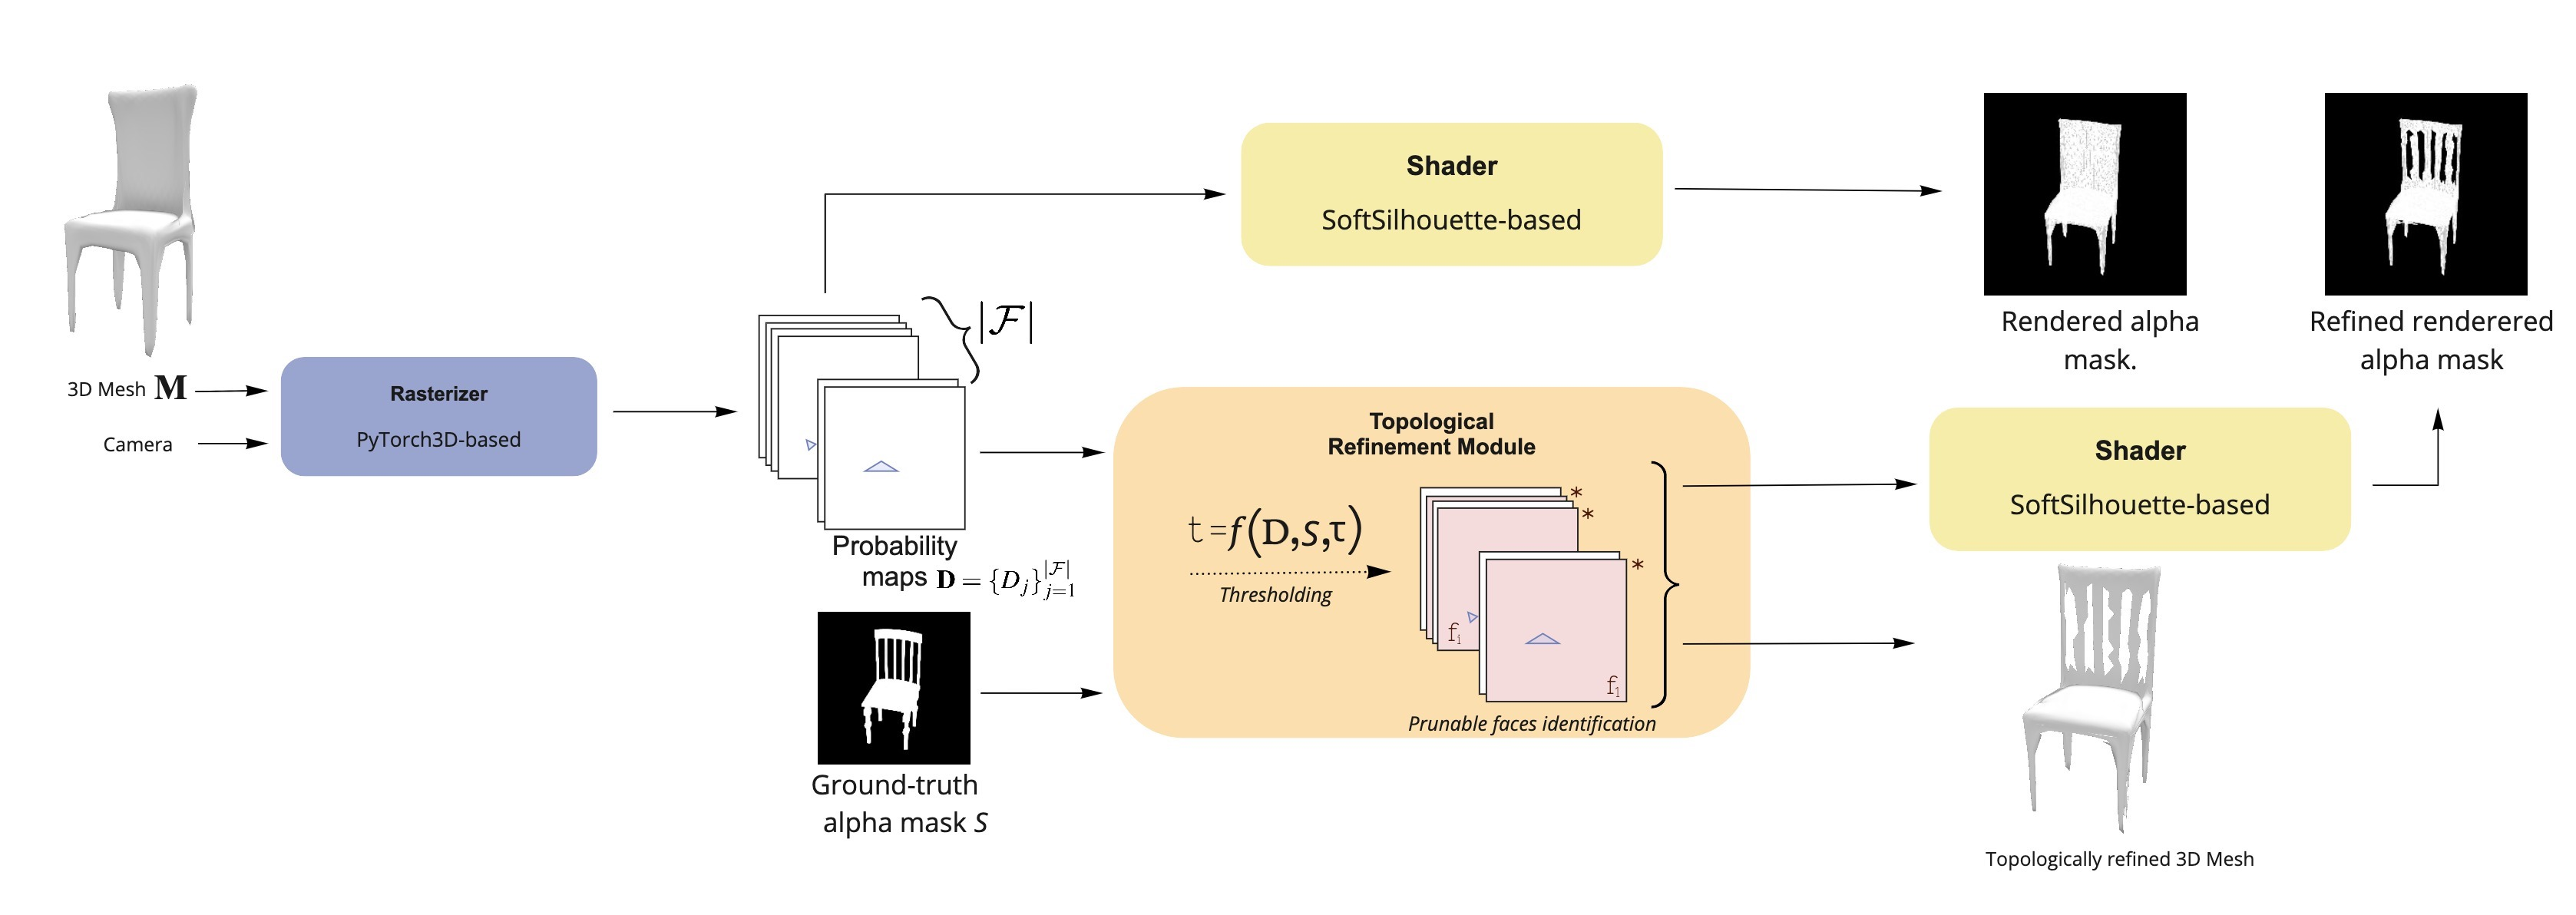
\includegraphics[width=13cm]{images/adaptativesr/final_figure.jpg}
\end{center}
    \caption{Architecture overview of our method. \textit{Based on a 3D mesh} \textbf{M} \textit{and a camera pose information, our module leverages onto PyTorch3D rasterizer to detect and prune onto the mesh surface by only getting consideration for the ground-truth alpha mask S}}
\label{fig:pipeline_overview}
\end{figure*}

Detecting those faces can be made through the computation of an Intersection over Union (IoU) score between the face from F involved in the rendering of \textbf{M} and the ground-truth alpha mask \textit{S}. Those faces can then be removed from the 3D mesh surface or directly discarded in the shader stage of the renderer. Inspired by the thresholding strategy introduced in \citep{pan2019deep}, we set an adaptative threshold $\tau$ based on the IoU score distribution and quantile $Q_{\tau}$ where $\tau \in [0,1]$.

\begin{equation}
    \tau=Q_{\tau}({\gamma/\Gamma})
\end{equation}

where ${\gamma/\Gamma}$ refers to the IoU distribution score. 
In a similar fashion line to what \citep{pan2019deep} did for the thresholding strategy in their pipeline architecture, the setting of $\tau$ influences the number of pruned faces: the lower $\tau$ is, the lower the number of faces detected as wrongly projected will be.

\paragraph{Implementation details.}
We implement our topological refinement strategy onto the renderer from the PyTorch3D \citep{ravi2020accelarating} library. The renderer's modularity offered by \citep{ravi2020accelarating} is worth mentioning since the entire rendering procedure can be adjusted as desired. We paid attention to its rasterization stage in our work for its connivance with the one from SoftRasterizer \citep{liu2019soft}. 

One of the core differences it exists between those two frameworks in the silhouette rasterization process concerns the number of faces involved: while PyTorch3D only considers for each pixel location $p_i$ the top-\textit{K} closest faces from the camera center of \textbf{M}, SoftRasterizer equally considers all the faces. 
We denote by $\mathbf{P}\in \mathbb{R}^{K\times(H\times W)}$ the intermediate probability map produced by \citep{ravi2020accelarating} which is highly related to the one originally introduced in \citep{liu2019soft}. Considering any 2D pixel location $p_{i}=(x_{i};y_{i}) \in \{0,..H-1\}\times\in \{0,..W-1\} $ and the $k^{th}$ closest face $f_{k}^{i}$, the distance based probability tensor $\mathbf{P}$ is expressed through:

\begin{equation}
    \mathbf{P}[k,p_{i}]=\left(1+e^{-d(f_{k}^{i},p_{i})/\sigma}\right)^{-1} 
\end{equation}

where $d(f_{k}^{i},p_{i})$ stands for the Euclidean distance between $p_i$ and $f_{k}^{i}$, while $\sigma$ is a hyperparameter to control the sharpness of the rendered silhouette image. Both $d$ and $\sigma$ have been defined in SoftRasterizer \citep{liu2019soft}. \newline

We consider the same soft silhouette shader stage as the one introduced in SoftRasterizer to obtain the soft alpha mask $\hat{S}$ from $\mathbf{P}$ through the aggregation function:

\begin{equation}
    \hat{S}[p_i]=1 - \prod_{k=1}^{K} (1 - \mathbf{P}[k,p_{i}])
\end{equation}

It is worth to emphasise the indexing notation in $\mathbf{P}$. Indeed, face indexes $f_{k}^{i}$ and $f_{k'}^{i'}$, $\{i,k\} \neq \{i',k'\}$ might refer to the same physical face on \textbf{M} because a rendered face is likely to cover an area larger than a single pixel. 

We introduced $\mathcal{F}$ as the set of unique faces involved in the rendering of any mesh \textbf{M} obtained from $\mathbf{P}$. The larger K is, the more likely the cardinality of $\mathcal{F}$ will get close to the total number of faces in the original mesh $|F|$. 

Finally and because $\mathbf{P}$ is not exactly designed in the same way as SoftRasterizer did, we denote by $\mathbf{D}=\{D_{j}\}_{j=1}^{|\mathcal{F}|}\in \mathbb{R}^{|\mathcal{F}|\times(H\times W)}$ the same probability map tensor as defined in \citep{liu2019soft}.

The way our module determined whether or not a face should be pruned is conditioned by the degree of overlap between the ground truth alpha mask \textit{S} and the rendered face. Since each face $f_{j} \in \mathcal{F}$ contributes to the final rendered silhouette through its probability map $D_{j}\in \mathbb{R}^{(H\times W)}$, an Intersection over Union (IoU) term is computed: 

\begin{equation}
\begin{cases}
     \gamma_{j}=\sum_{p_{i}\in S} \min \left(  D_{j}[p_{i}] , S[p_{i}] \right) \\
     \Gamma_{j}=\sum_{p_{i}\in S} \max \left( D_{j}[p_{i}],S[p_{i}] \right)
\end{cases}
\end{equation}

The ratio $\gamma_{j}/\Gamma_{j}$ gives the well-known IoU score. We extend the computation for a single face $f_{j}$ to all the faces from $\mathcal{F}$, and we note $\gamma/\Gamma \in \mathbb{R}^{|\mathcal{F}|}$ the complete IoU score distribution.

Our method finally leverages onto this distribution score to determine the faces which should be pruned on $\mathbf{M}$. We adopt a thresholding strategy partially inspired from \citep{pan2019deep} and set an adaptative threshold $t$ based on statistical quantile consideration: faces with a lower IoU score than $t=Q_{\tau}(\gamma/\Gamma)$ are pruned from $\mathbf{M}$. Such a choice allows to dynamically adapt the number of faces to prune based on the IoU distribution. 

\subsection{Experiments}
\label{sec:experiments}

\textbf{Dataset} Our approach has been extensively tested with the ShapeNetCore \citep{chang2015shapenet}. In line with the work from by TMN \citep{pan2019deep}, our experiments are thus restricted to the topologically challenging "chair" class from \citep{chang2015shapenet}. It contains a total of 6774 different chairs, with 1356 instances in the testing set.

\noindent\textbf{Metrics} We evaluate our method through both qualitative and quantitative considerations. We use the 2D IoU metric to assess how well the refined mesh produced by our module better match the ground truth alpha mask compared to the topologically non-refined mesh. We also use 3D metrics with the Chamfer Distance (CD), F-Score and METRO distance to evaluate our method. The METRO criterion is first introduced in \citep{cignoni1998metro} and reconsidered in Thibault Groueix \etal 's AtlasNet \citep{groueix2018papier} work. Its use is motivated by its consideration for mesh connectivity contrary to the CD or F-score metric that only reason onto 3D point clouds distribution. 


\noindent\textbf{3D Mesh generation network} Our refinement module can be integrated into any image-based 3D reconstruction pipeline and is thus agnostic to the network responsible for producing the 3D mesh. We chose to work with the meshes generated by \citep{pan2019deep} and thus trained it with the training set from \citep{chang2015shapenet}. Since we only want to focus on face-pruning considerations, we only train the ResNet18 encoder with the first stage of their 3D mesh reconstruction architecture, referred to as \textit{SubNet-1} in \citep{pan2019deep} and abbreviated as TMN in this section. The TMN architecture thus consists of a deformation network and a learnt topological modification module. It is worth mentioning the TMN \citep{pan2019deep} architecture has been trained and used for inference with the provided ground truth labels and rendered images from 3D-R2N2 \citep{choy20163d}. We called "Baseline" the deformation network preceding the topology modification network \citep{pan2019deep}. The genus-0 3D mesh produced by the Baseline network has been obtained from a 3D sphere template with 2562 vertices. 


\noindent\textbf{PyTorch3D Renderer} We use the PyTorch3D \citep{nie2020total3dunderstanding} differentiable renderer and set K=30 and $\sigma=5.10^{-7}$ to get the alpha mask as sharp as possible. All the 2D alpha masks, size 224x224, involved in this Experiments section were obtained with the PyTorch3D renderer and have been centred. Similarly to what \citep{choy20163d,liu2019soft,yan2016perspective} did for the rendering silhouette masks, we considered 24 views per meshes with a fixed camera distance $d_{camera}=2.732m$ and an elevation angle set to $30\degree$. The azimuth angle varies by an increment of $15\degree$ from $0\degree$ to $345\degree$. All the meshes predicted by pan2019deep \citep{pan2019deep} were normalised in the same way as ShapeNetCore\citep{chang2015shapenet}. 

We both present qualitative and quantitative results of our pruning based method through 2D and 3D evaluation considerations. We demonstrate how effective our method can be by only leveraging on 2D alpha masks and the renderer modularity. 

\paragraph{Topological refinement evaluation - Qualitative results}

We aim first to highlight to which extent we can detect the relevant faces on the 3D mesh that might be pruned during the rendering. Figure \ref{fig:face2prune} highlights the faces considered as wrongly rendered compared to the ground-truth alpha mask on three different chairs. Based on these 2D silhouette considerations, we achieve visually more appealing results than \citep{pan2019deep}. 

\begin{figure*}[htb]%[htp!]
\begin{center}
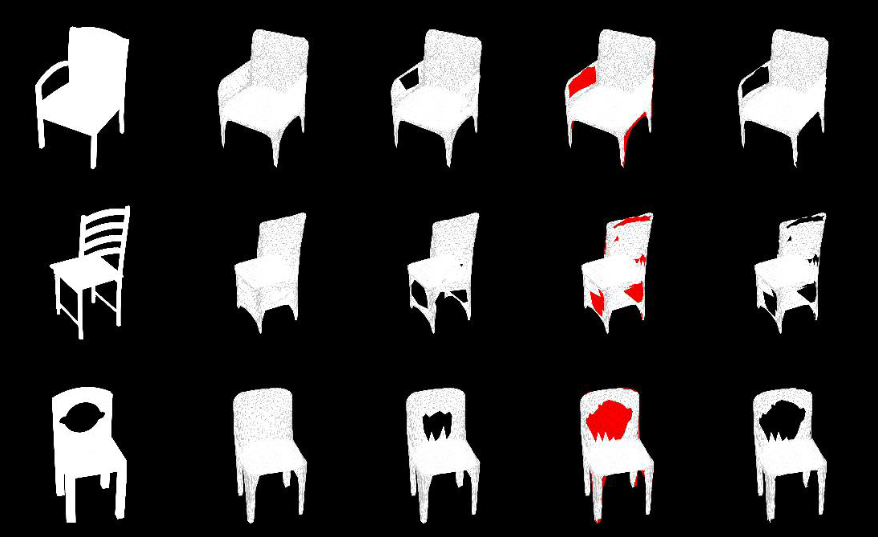
\includegraphics[width=8cm]{images/adaptativesr/highlight_faces.png}
\end{center}
    \caption{Silhouette based comparison on several instance from the ShapeNetCore test set. \textit{Faces rendered onto red regions should be pruned on 3D mesh surface} - $\tau = $ \textbf{0.05} - From left to right: Ground-Truth, Baseline, TMN\citep{pan2019deep}, Ours with highlighted faces to prune, Ours final result.}
\label{fig:face2prune}
\end{figure*}

The Figure \ref{fig:pruning_multi_view} somehow extends the later observation through 6 different viewpoints from the same chair instance. In this specific example, the TMN pruning module failed to detect some faces to prune. It produced the same mesh as the baseline one, while our method successfully pruned the faces that were rendered the worst, according to the ground truth alpha mask. The faces that are pruned on each view are independent of the other viewpoints. 

\begin{figure*}[h!]%[htp!]
\begin{center}
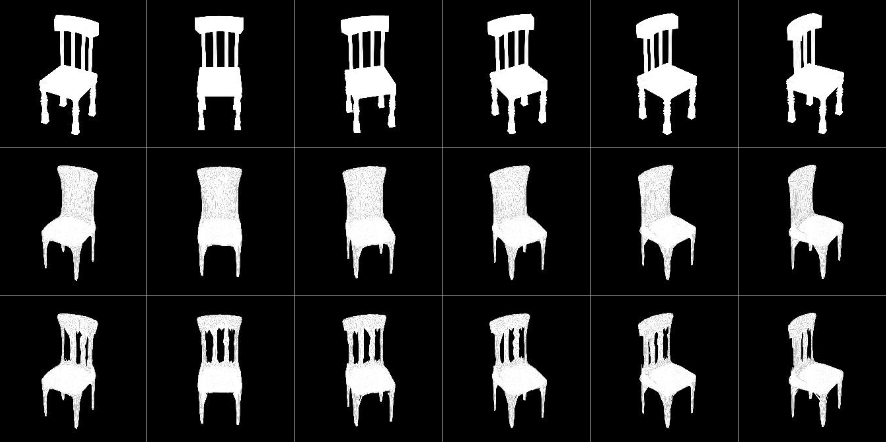
\includegraphics[width=8.cm]{images/adaptativesr/severalview2D.png}
\end{center}
    \caption{Rendered silhouette mask results on 6 viewpoints - $\tau =\textbf{0.05}$ - From top to bottom: Ground-Truth, TMN\citep{pan2019deep},  Ours}
\label{fig:pruning_multi_view}
\end{figure*}

Even the viewpoint associated to a tricky azimuth angle as the one depicted in the last column is informative enough for our module to remove the relevant faces during rendering.

\paragraph{2D and 3D-based quantitative evaluation}

We compare the performances of our method through different threshold $\tau$ on Table \ref{tab:sota_table} with both the meshes produced by the Baseline network and TMN\citep{pan2019deep}. From the 1356 inferred meshes in the ShapeNetCore\citep{chang2015shapenet} test set, we manually selected 50 highly challenging meshes (from a topological perspective) and render them through the 24 different camera viewpoints we described earlier with the PyTorch3D's renderer. The threshold associated to the F-score has been set to 0.001. A total number of N=10.000 points have been uniformly sampled over the different meshes surface to compute the 3D metrics. 

\begin{table}[htp!]
\begin{center}
\caption{2D and 3D-based metric scores comparison with the Baseline and TMN\citep{pan2019deep} - \textit{Presented results were averaged over the 50 instance from our manually curated test set and over the 24 different viewpoints for the 3D metrics.}} 
\label{tab:sota_table}

\begin{tabular}{|l|c|c|c|c|}
\hline
\textit{Method} & 2D IoU $\uparrow$   & CD $\downarrow$  &F-Score $\uparrow$ & METRO $\downarrow$ \\ 
 \hline\hline
Baseline & 0.660  &  6.602  & 53.27  &  1.419      \\ 
\hline
TMN\citep{pan2019deep} & 0.681  & \textbf{6.328}   & \textbf{54.23}  & \textbf{1.293} \\ 
\hline
Ours $\scriptstyle \tau=0.01$ & 0.747 & 6.541  &  53.39 &  1.418      \\
\hline
Ours $\scriptstyle \tau=0.03$ & 0.755 &6.539  & 53.39  &    1.417  \\
\hline
Ours $\scriptstyle \tau=0.05$ & 0.763 & 6.540  &   53.34 &   1.417     \\
\hline
Ours $\scriptstyle \tau=0.1$ & \textbf{0.778} & 6.551  & 53.27 &  1.416     \\
\hline
Ours $\scriptstyle \tau=0.15$ & 0.771 & 6.548  & 53.26  &    1.416   \\
\hline

%
\end{tabular}
\end{center}

\end{table}

Our method outperforms the learned topology modification network from TMN\citep{pan2019deep} according to Table \ref{tab:sota_table} when compared using the 2D IoU score. It is worth re-mentioning that the presented results for TMN\citep{pan2019deep} only come from the very first learned topological modification network and thus do not consider the topological refinement from the \textit{SubNet-2} and \textit{SubNet-3} network. Whereas none of our configurations (with different $\tau$ values) succeed to reach better scores on 3D metrics than TMN\citep{pan2019deep}, we stress on two points: \begin{enumerate}
    \item Topologically refined mesh by our method always get better results than the ones produced by the Baseline. 
    \item Our face-pruning strategy only relies on a single 2D alpha mask and does not required any form of 3D-supervised compared to \citep{pan2019deep}. 
\end{enumerate}

Since the method we designed only relies on 2D considerations, the camera viewpoint we considered to perform the topological refinement must influence the different evaluation metrics. We show in Figure \ref{fig:pruning_viewpoint_influence} to which extent the camera pose affects both the 2D IoU and the CD scores.


\begin{figure}[h!]
  \centering
  \subfloat[a][2D IoU]{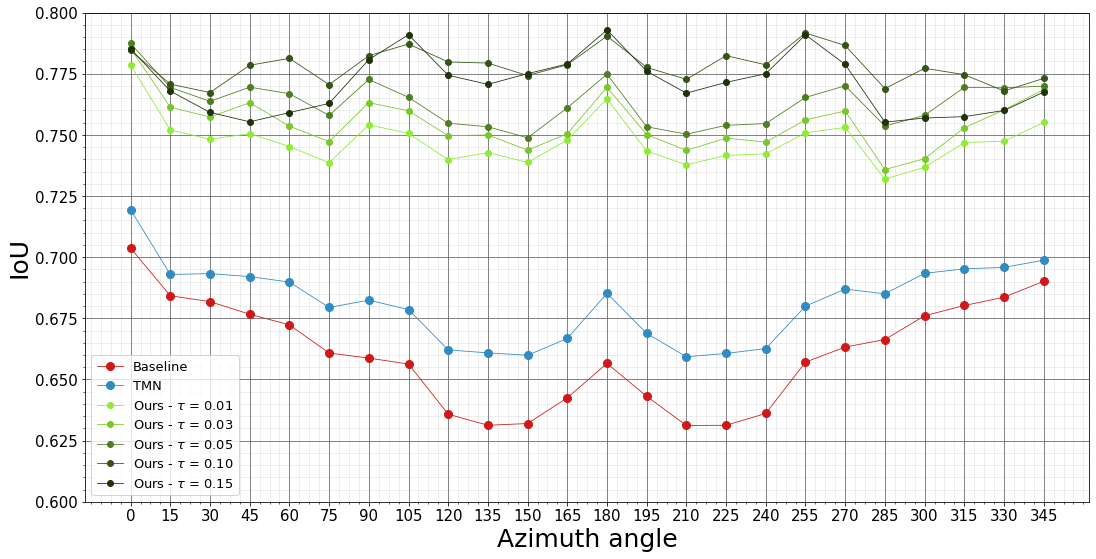
\includegraphics[width=8cm]{images/adaptativesr/multiviewsPLOT.png} \label{fig:a}} \\
  \subfloat[b][Chamfer distance]{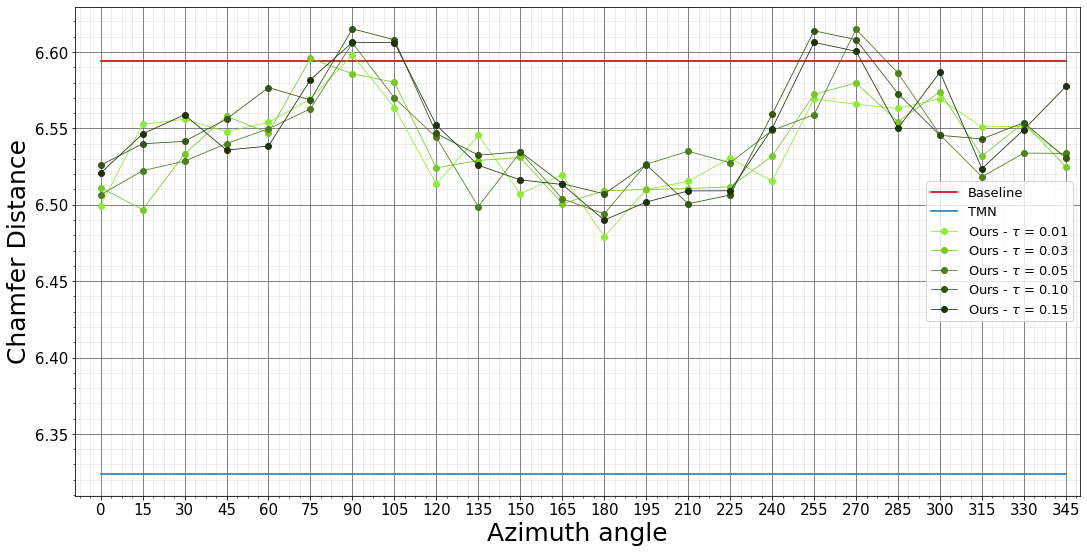
\includegraphics[width=8cm]{images/adaptativesr/plot_Chamfer_Distance_last.png} \label{fig:b}}
  \caption{Camera viewpoint influence over the 2D IoU (top, (a)) and Chamfer distance (bottom, (b) scores.} \label{fig:pruning_viewpoint_influence}
\end{figure}


Azimuth angles around the symmetrical pair $\{90^{\degree}, 270^{\degree}\}$ are more challenging since there are not as informative as the viewpoints closed to $180^{\degree}$. Indeed, our method struggles to get better results than the Baseline on these cases. Our test set is slightly imbalanced since it only contains few chair instances where armrests require topological refinement and conversely a greater number with topologically complex back parts. Our method thus slightly performs worse than the Baseline on around both $90^{\degree}$ and $270^{\degree}$ angles as complex chairs' back structures are invisible on these viewpoints. 

We finally also quantitatively confirm the intuited impact of $\tau$ during the rendering process on the 2D IoU score: the higher $\tau$ is, the larger the number of faces we discarded. 


\subsection{Limitations and further work}



Our method shows encouraging results in 3D meshes topological refinement through 2D alpha mask considerations but has few remaining limitations. First regarding the thresholding strategy we used to determine whether or not a face should be pruned on the 3D mesh surface. While we require to set a fixed hyperparameter - $\tau$ - in our method as \citep{pan2019deep} did, we align with \citep{nie2020total3dunderstanding} on the importance to rely on local 2D and 3D prior information to propose a clever and more robust thresholding strategy. Moreover, our module might also incorrectly behave on the rendered faces closed to the silhouette boundary edges. 

From a broader work perspective, our method currently relies on alpha masks and thus leaves behind texture information from RGB images. While impressive 3D textured results exist with UV mapping on self-supervised image-based 3D reconstruction methods with genus-0 meshes\citep{li2020self,pavllo2020convolutional}, no attempts have been made to the best of our knowledge to go beyond such 0 order. Finally and since our work is completely agnostic to the 3D mesh reconstruction network, a natural next move would go for the design of a complete self-supervised 3D reconstruction pipeline where our topological refinement module is including. 

\subsection{Conclusion}
\label{sec:conclusion}
We proposed a new way to perform topological refinement onto 3D meshes surface by only getting consideration for 2D alpha mask and the modularity of the PyTorch3D rasterization framework. To the best of our knowledge, no attempt has been made in our line of work since both TMN\citep{pan2019deep} and Total3D\citep{nie2020total3dunderstanding} respectively perform faces and edges pruning through 3D-supervised  neural networks. In this way, our work introduced a new research path to address the 3D mesh topology refinement issue. The agnostic design of our method allows any self-supervised image-based 3D reconstruction pipeline - based on the PyTorch3D renderer framework - to leverage the work we presented in this paper to reconstruct topologically complex meshes. We obtained consistent and competitive results from a topological perspective compared to the 3D-based pruning strategy from \citep{pan2019deep}. 








\section{Details on Assets used in Chapter~\ref{chapter:epipolarnvs}}
\label{sec:GradPaint assets}



Table \ref{tab:linkschap3} (links) and Table \ref{tab:licenceschap3} (licences)
list the assets we used in this work.

\begin{table*}[h]
\hspace{\sizeforappendix}
\footnotesize
\begin{tabular}{lll}
\toprule
\textbf{Asset Name} & \textbf{Link} \\
\midrule
% datasets 
CelebA & https://mmlab.ie.cuhk.edu.hk/projects/CelebA.html \\
FFHQ &  https://github.com/NVlabs/ffhq-dataset \\
Places2 &  http://places2.csail.mit.edu/download.html \\
ImageNet & https://www.image-net.org \\
COCO & https://cocodataset.org/ \\
Guided Diffusion & https://github.com/openai/guided-diffusion \\
Latent Diffusion & https://github.com/CompVis/latent-diffusion \\
Stable Diffusion & https://github.com/CompVis/stable-diffusion \\
LaMa & https://github.com/advimman/lama \\
Palette & https://github.com/Janspiry/Palette-Image-to-Image-Diffusion-Models \\
LPIPS &  https://github.com/richzhang/PerceptualSimilarity\\
FID & https://github.com/mseitzer/pytorch-fid \\ % code and moels
FFHQ pre-trained model & https://github.com/yandex-research/ddpm-segmentation \\ % just model
RePaint & https://github.com/andreas128/RePaint\\
MCG & https://github.com/HJ-harry/MCG\_diffusion\\
\bottomrule
\end{tabular}
\caption{List of asset links.}
\label{tab:linkschap3}
\end{table*}


\begin{table*}[h]
\hspace{\sizeforappendix}
\footnotesize
\begin{tabular}{lll}
\toprule
\textbf{Asset Name} & \textbf{Asset type} & \textbf{License} \\
\midrule
CelebA & Images & CC BY-NC-SA 4.0 License \\
FFHQ & Images &  https://github.com/NVlabs/ffhq-dataset/blob/master/LICENSE.txt \\
Places2 &  Images & Creative Commons Attribution 4.0 International \\
ImageNet & Images & https://www.image-net.org/download.php \\
COCO & Images & Creative Commons Attribution 4.0 License \\
Guided Diffusion & Code and Models & MIT License\\
Latent Diffusion & Code and Models & MIT License \\
Stable Diffusion & Code and Model & CreativeML Open RAIL-M\\
LaMa & Code and Models & Apache License 2.0 \\
Palette & Code and Models & MIT License \\
LPIPS & Code and Models & BSD-2-Clause License \\
FID & Code and Models & Apache-2.0 License \\
FFHQ pre-trained model & Model & MIT License \\% just model
RePaint & Code & CC BY-NC-SA 4.0 License\\
MCG & Code & Apache License 2.0\\
\bottomrule
\end{tabular}
\caption{List of asset licenses.}
\label{tab:licenceschap3}
\end{table*}
\cleardoublepage
\let\leftmark=\oldleftmark

\end{document}
